%%%%%%%%%%%%%%%%%%%%%%%%%%%%
% Reporte Técnico Trabajo Terminal II                          
% Traveler Assistant System For Mexico City (TASMC)
%													   
% Autores:
% Erick Rafael Vivanco Carmona 
% Sergio Barajas Uribe
%%%%%%%%%%%%%%%%%%%%%%%%%%%%

%----------------------------------------------------------------------------------------
%	Paquetes y configuración
%----------------------------------------------------------------------------------------

\documentclass[12pt, oneside]{Thesis}
\usepackage{times}
\usepackage[spanish]{babel}
\usepackage{multirow}
\usepackage{color, colortbl}
\usepackage{booktabs}
\usepackage{titlesec}
\setcounter{secnumdepth}{5}

\titleformat{\paragraph}
{\normalfont\normalsize\bfseries}{\theparagraph}{1em}{}
\titleformat{\subparagraph}
{\normalfont\normalsize\bfseries}{\theparagraph}{1em}{}
\titlespacing*{\paragraph}
{0pt}{3.25ex plus 1ex minus .2ex}{1.5ex plus .2ex}
\titlespacing*{\subparagraph}
{0pt}{3.25ex plus 1ex minus .2ex}{1.5ex plus .2ex}

\graphicspath{{Imagenes/}}

\usepackage[square, numbers, comma, sort&compress]{natbib} 
\hypersetup{urlcolor=black, colorlinks=true} 
\title{\ttitle} % Defines the thesis title - don't touch this

\begin{document}

\frontmatter % Use roman page numbering style (i, ii, iii, iv...) for the pre-content pages	

\setstretch{1.3} % Line spacing of 1.3

% Define the page headers using the FancyHdr package and set up for one-sided printing
\fancyhead{} % Clears all page headers and footers
\rhead{\thepage} % Sets the right side header to show the page number
\lhead{} % Clears the left side page header

\pagestyle{fancy} % Finally, use the "fancy" page style to implement the FancyHdr headers

\definecolor{azul}{RGB}{74,126,187}

\newcommand{\HRule}{\rule{\linewidth}{0.5mm}} % New command to make the lines in the title page
\renewcommand{\listtablename}{Índice de tablas}
\renewcommand{\tablename}{Tabla}
\newcommand{\latexcolumnseprulecolor}{\color{azul}}

% PDF meta-data
\hypersetup{pdftitle={\ttitle}}
\hypersetup{pdfsubject=\subjectname}
\hypersetup{pdfauthor=\authornames}
\hypersetup{pdfkeywords=\keywordnames}

%----------------------------------------------------------------------------------------
%	Portada
%----------------------------------------------------------------------------------------

\thispagestyle{empty}

\begin{minipage}[c][0.1\textheight][c]{0.2\textwidth}
	\begin{center}
    		
\includegraphics[height=3cm]{portada/ipnC.jpg}
	\end{center}
\end{minipage}
\begin{minipage}[c]{0.8\textwidth}
	\begin{center}
		{\fontsize{18}{28}\selectfont \bf INSTITUTO POLITÉCNICO NACIONAL}
		{\fontsize{15}{25}\selectfont \bf ESCUELA SUPERIOR DE CÓMPUTO}
	\end{center}
\end{minipage}

\begin{minipage}[c][0.8\textheight][t]{0.2\textwidth}
\begin{center}
        \hskip2pt
    	    \latexcolumnseprulecolor \vrule width2pt height19.3cm
        \hskip0.6mm
	   \vrule width3.5pt height19.3cm
        \hskip0.6mm
        \vrule width2pt height19.3cm \\
        
\includegraphics[height=2.1cm]{portada/escomC.jpg}
        \end{center}
\end{minipage}
\begin{minipage}[c][0.8\textheight][c]{0.8\textwidth}
	\begin{center}
   		\vspace{2cm}
    		{\fontsize{19}{29}\selectfont \bf ESCOM}\\
    		\vspace{1.5cm}
	    {\fontsize{14}{24}\selectfont Trabajo Terminal}\\
	    \vspace{0.3cm}
	    {\fontsize{16}{26}\selectfont \bf ``Traveler Assistant System For Mexico City (TASMC)''}\\
	    \vspace{0.3cm}
	    {\fontsize{14}{24}\selectfont 2014-A021}\\
	    \vspace{1cm}
	    {\fontsize{14}{24}\selectfont Presentan}\\
	    \vspace{0.1cm}
	    {\fontsize{15}{25}\selectfont \bf Barajas Uribe Sergio}\\
	    \vspace{0.1cm}
	    {\fontsize{15}{25}\selectfont \bf Vivanco Carmona Erick Rafael}\\
	    \vspace{1cm}
	    {\fontsize{14}{24}\selectfont Directores}\\
	    \vspace{0.1cm}
	\end{center}
	\begin{tabular}{>{\centering}p{5cm}p{1cm}>{\centering}p{5cm}}
		{\centering \fontsize{15}{25}\selectfont \bf M. en C. Macario Hernández Cruz} &
	    	& {\centering \fontsize{15}{25}\selectfont \bf M. en C. Axel Ernesto Moreno Cervantes}\\
	\end{tabular}
	\vspace{5cm}
	\begin{flushright}
		{\fontsize{14}{24}\selectfont Junio, 2015}\\	
	\end{flushright}
\end{minipage}
\thispagestyle{empty}

\begin{center}
	\begin{tabular}{lcl}
		\multirow{5}{*}{
\includegraphics[height=3cm]{portada/ipn.jpg}} &
		&
      	\multirow{3}{*}{
\includegraphics[height=2.8cm]{portada/escom.jpg}}\\
      	& \large \bf INSTITUTO POLITÉCNICO NACIONAL & \\
      	& \large \bf ESCUELA SUPERIOR DE CÓMPUTO &\\
      	& \large \bf SUBDIRECCIÓN ACADÉMICA &
	\end{tabular}
\end{center}

\vspace{0.5cm}

\centerline{\large No. de Registro: 2014-A021}
\centerline{\large Documento técnico}

\vspace{0.8cm}

\centerline{\Large \bf Traveler Assistant System For Mexico City (TASMC)}

\vspace{0.8cm}

\centerline{\large Presentan}

\vspace{0.3cm}

\centerline{\large \bf Barajas Uribe Sergio \footnote{E-mail: scscf.1992@gmail.com}}
\centerline{\large \bf Vivanco Carmona Erick Rafael \footnote{E-mail: erickvivanco01@hotmail.com}}

\vspace{0.5cm}

\centerline{\large Directores}

\vspace{0.3cm}

\centerline{\large \bf M. en C. Macario Hernández Cruz}
\centerline{\large \bf M. en C. Axel Ernesto Moreno Cervantes}

\vspace{0.8cm}

\centerline{\Large Resumen}

El presente proyecto TASMC, consta del desarrollo de un sistema de información que tendrá como propósito proporcionar al usuario lo necesario para hacer posible la organización integral del viaje aéreo, con carácter turístico o de negocios, en el Aeropuerto Internacional de la Ciudad de México (AICM), suministrando en un dispositivo móvil funciones que serán desarrolladas en dos fases: la primera corresponde a la ubicación de los servicios dentro del aeropuerto; la segunda fase corresponde a la construcción de bases de información para seleccionar la mejor opción  de vuelos, hoteles, sugerencia de rutas al aeropuerto a través de mapas, información de vuelos en lo que respecta a salidas y llegadas, indicando puerta de salida y banda de equipaje; así como el seguimiento de vuelos a través de localización en mapas por longitud y latitud desde su origen hasta la llegada del vuelo a su destino.

\vspace{0.2cm}

\centerline{\textbf{Palabras Clave }- Aplicaciones Móviles, Geolocalización, Aplicaciones Web e Ingeniería de Software}
\thispagestyle{empty}
\vspace*{\fill}
	\centerline{\fontsize{19}{29}\selectfont \bf Advertencia}
	\begin{figure}[htbp]
		\centering
		
\includegraphics[width=1\textwidth]{Figuras/advertencia.png}
	\end{figure}
\vspace*{\fill}

%----------------------------------------------------------------------------------------
%	LIST OF CONTENTS/FIGURES/TABLES PAGES
%----------------------------------------------------------------------------------------

\pagestyle{fancy}

\lhead{\emph{Índice general}} 
\tableofcontents % Write out the Table of Contents

\lhead{\emph{Índice de figuras}} 
\listoffigures % Write out the List of Figures

\lhead{\emph{Índice de tablas}} 
\listoftables % Write out the List of Tables

%----------------------------------------------------------------------------------------
%	Contenido
%----------------------------------------------------------------------------------------

\mainmatter % Begin numeric (1,2,3...) page numbering

\pagestyle{fancy} % Return the page headers back to the "fancy" style

% Capitulo 1

\chapter{Introducción} % Main chapter title

\label{Introduccion} % For referencing the chapter elsewhere, use \ref{Chapter1} 

\lhead{Capítulo 1 \emph{Introducción}} % This is for the header on each page - perhaps a shortened title

%----------------------------------------------------------------------------------------

En la actualidad, un dispositivo móvil está presente en los procesos de decisión en buena parte de lo que hacemos. Por ejemplo: es el aparato que nos despierta, y es el principal canal de comunicación en nuestra vida tanto profesional, como personal.

El presente proyecto describe el desarrollo de la aplicación Traveler Assistant System For Mexico City (TASMC), se basa en dos factores que han influido de forma decisiva en la experiencia viajera: el incremento en la transportación aérea de pasajeros; así como la creciente utilización de los dispositivos móviles, y con ellos, la facilidad de encontrar y comparar precios para elegir los más convenientes de acuerdo a las posibilidades de cada persona, y con ello, la opción de personalizar al máximo los viajes. La planeación es la mejor manera de ahorrar dinero y tiempo en un viaje. La incorporación de un elemento como el móvil conectado a internet, añade  nuevos fenómenos que enriquecen la experiencia viajera; un ejemplo de dichos fenómenos es el acceso a numerosos servicios de geolocalización.

El sector turístico es uno de los que se han visto obligados a adaptarse a los nuevos usos de los dispositivos móviles. Las nuevas tecnologías han proporcionado al cliente de las agencias de viajes, líneas aéreas, y servicios de hotelería, una gran autonomía \cite{appsVIajar} para organizar sus viajes. De acuerdo a la encuesta nacional de ingresos y gastos de los hogares “ENIGH 2012” y el modulo de disponibilidad y uso de tecnología de la información en los hogares “MODUTIH 2012” la conectividad es de un 60\% en los dispositivos móviles provocando un cambio sustancial en el proceso tradicional de gestión de un viaje aéreo \cite{endutih}.

El proyecto que se plantea será diseñado y desarrollado para dispositivos móviles en dos fases: como primera fase, localizar espacios o servicios en un área predeterminada, estos puntos se mostraran con etiquetas dentro del plano arquitectónico. Inicialmente para facilitar la gestión del módulo de la aplicación, el ámbito se limitará a la terminal 1 del AICM. Como segunda fase, hacer posible la planeación y organización integral de viajes aéreos, incluyendo información del vuelo, relación de vuelos y hoteles, itinerario de actividades planeadas, listado para control de equipaje y seguimiento de vuelos a través de mapas.


%----------------------------------------------------------------------------------------
\section{Problemática}

Los viajeros tienen ciertas necesidades desde el momento que deciden viajar por el transporte aéreo, incluso deben considerar una serie de problemas que se les pueden presentar como se muestra a continuación:

\textbf{Necesidades:}

\begin{itemize}
	\item Conocer el precio y horario de los vuelos que los llevan a su destino.
	\item Buscar un hotel de su conveniencia para hospedarse.
	\item Hacer un itinerario de viaje.
\end{itemize}

\textbf{Problemas:}

\begin{itemize}
	\item Olvidar papeles importantes, como el pasaporte.
	\item Olvidar empacar algún objeto que les sea necesario.
	\item Llegar a destiempo a la cita en el aeropuerto debido a la falta de conocimiento de la ruta.
	\item No ubicarse correctamente dentro del aeropuerto.
\end{itemize}

Hoy en día los viajeros buscan la información para cubrir estas necesidades utilizando la Internet,  generalmente lo hacen visitando diferentes páginas Web para encontrar la opción que mejor se ajuste a sus necesidades. Por otro lado, los problemas que se muestran no siempre son considerados y llevan a consecuencias no muy agradables como el perder un vuelo.
\section{Solución Propuesta}

Tomando en cuenta las problematicas mensionadas, se plantea desarrollar una solución que permita al viajero aéreo de la Ciudad de México organizar de manera adecuada su viaje, ofreciendo así una herramienta útil para el ámbito de turismo en México.

La herramienta a desarrollar tendrá la arquitectura que se muestra en la Figura \ref{fig:Arquitectura}. 

\begin{figure}[htbp]
	\centering
		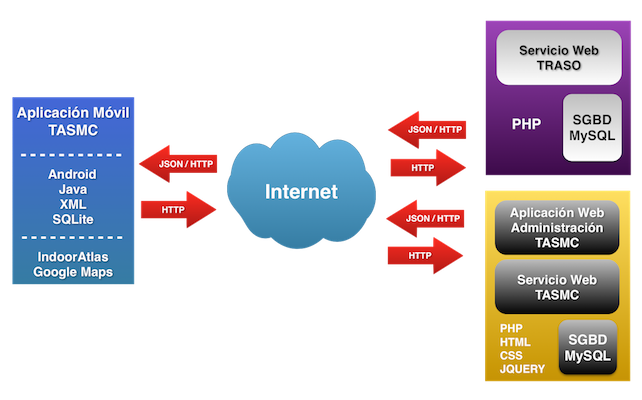
\includegraphics{Figuras/arquitectura.png}
		\rule{35em}{0.5pt}
	\caption[Diagrama de Arquitectura de TASMC]{Diagrama de Arquitectura de TASMC.}
	\label{fig:Arquitectura}
\end{figure}

A continuación se describe cada uno de los componentes que se muestran en la Figura \ref{fig:Arquitectura}:

\begin{itemize}
	\item \textbf{Dispositivo Móvil: }Cuenta con diferentes tecnologías que serán aprovechadas para el desarrollo de la aplicación, por lo tanto, la aplicación móvil será instalada en este dispositivo. Se conectará a la Internet para tener comunicación con el Web Service externo y con el que se desarrollará para este sistema.
	\item \textbf{Web Services: }Se visualizan dos en la Figura \ref{fig:Arquitectura}, uno es el externo que nos brindará la información correspondiente a hoteles y vuelos, y el otro que se desarrollará para brindar la información de los usuarios que utilizan la aplicación. 
	\item \textbf{Servidores: }Observamos dos en la Figura \ref{fig:Arquitectura} que son donde se alojan los Web Services y las Bases de Datos correspondientes, en el servidor TASMC también habrá aplicación Web.
	\item \textbf{Bases de Datos: }En este módulo encontramos los datos que se proveerán a la aplicación móvil y la aplicación Web.
	\item \textbf{Aplicación Web: }Es una aplicación que servirá para administrar a los usuarios, lugares y objetos de equipaje de la aplicación móvil.
\end{itemize}
\section{Alcances y Limitaciones}

El trabajo terminal tiene como alcance implementar una aplicación móvil que sea capaz de ubicar al usuario en el AICM, ayudando al mismo a encontrar la terminal y la sala en donde será su salida. También podrá localizar sitios de interés como alimentos y bebidas, compras, comunicaciones, servicios financieros,  servicios médicos, transportación terrestre y servicios turísticos.

El proyecto puede tener mayor alcance, ya que se podría extender en un futuro con otras funciones como información detallada de los sitios de interés buscados por el usuario, ofertas y promociones de los locales disponibles, consultas de catálogos, trazado de rutas desde el origen del usuario hasta su destino, etc.

Las limitaciones que presenta el proyecto tienen que ver con la información que se pueda obtener, ya que puede no existir un servicio que nos brinde el acceso a la base de datos de las aerolíneas y hoteles. 

Otra de las limitaciones es la localización en interiores ya que sigue siendo objeto de un intenso estudio e investigación para brindar una mejor exactitud cuando se utiliza alguna tecnología con este fin.


\section{Objetivo General}

Diseñar un sistema integral de gestión para las actividades de los viajeros del AICM, al brindarles la información necesaria en su dispositivo móvil para hacer posible la organización integral de viajes turísticos o de negocios en México.
\section{Objetivos Específicos}

\begin{itemize}
	\item	Configurar el viaje dependiendo de gustos y posibilidades económicas del viajero.
	\item	Sugerir los vuelos disponibles.
	\item 	Sugerir hoteles disponibles. 
	\item	Sugerir diferentes objetos que debe portar el viajero dependiendo del tipo de viaje.
	\item	Proporcionar las herramientas que permitan al usuario generar un itinerario de viaje.
	\item	Sugerir la mejor ruta para llegar al aeropuerto.
	\item	Ubicar al viajero dentro del AICM.
	\item	Visualizar un panel con información del número de vuelo, estado del vuelo,  ciudades de origen y destino, hora de salida y llegada, fecha, terminal y puerta.
\end{itemize}
\section{Justificación}

TASMC te va a proporcionar listados de hoteles, vuelos y objetos que debes considerar en tu equipaje y facilidades para generar un itinerario, hasta este punto es prácticamente lo mismo que te ofrecen otras aplicaciones. Sin embargo, existen dos novedades que nos diferencian de dichas aplicaciones:

\begin{enumerate}
	\item La ruta más conveniente para llegar al aeropuerto que se sugerirá dependiendo la distancia del  trayecto utilizando un servicio externo de geolocalización, esto se puede obtener con otras aplicaciones dedicadas específicamente a rutas, nosotros lo brindamos en una misma aplicación dedicada a la gestión integral del viaje.
	\item El punto más novedoso de nuestro sistema es la "Localización en Interiores", esta rama de la localización aun no es tan utilizada por diferentes razones, una de ellas es que el GPS carece de un funcionamiento tan eficaz en interiores comparándolo con el desempeño en exteriores. Nuestro sistema será el primero que implemente la localización en interiores para el AICM.  
\end{enumerate}

Nuestro proyecto beneficiará a todos los viajeros aéreos del AICM, independientemente del tipo de viaje. Por ejemplo, un viajero que no visita constantemente el aeropuerto le será de mucha utilidad la localización en interiores ya que le facilitará encontrar su sala de abordaje de una manera eficaz. Por otro lado, una persona que visita constantemente el AICM puede ubicarse con facilidad pero de ninguna manera puede perder su vuelo, lo cual se evitará utilizando nuestra sugerencia de rutas al aeropuerto. Finalmente, lo que se quiere es que el usuario de nuestro sistema tenga una mejor planeación, organización y control de su viaje, además de un ahorro de tiempo, combustibles y dinero, lo que se logrará con la información que el sistema proporcionará a través del móvil.
 
Finalmente, con el desarrollo de este trabajo terminal se busca aprovechar y hacer frente a las siguientes observaciones:

\begin{itemize}
	\item El turismo en México es una actividad fundamental en el desarrollo económico del país.
	\item El turista se enfrenta a un problema que puede dificultar su viaje al no tener bien organizado el mismo.
\end{itemize}

El sistema estará orientado a dispositivos móviles debido al constante crecimiento en el número de usuarios de este tipo de dispositivos y al acelerado avance tecnológico en los sistemas móviles, en particular, el sistema estará disponible para dispositivos móviles con el sistema operativo Android, esto debido a que actualmente es el sistema operativo líder en el mercado (ver Figura \ref{fig:moviles})\cite{moviles} y ofrece una mayor flexibilidad para el desarrollo de aplicaciones en comparación con sus principales competidores.

\begin{figure}[htbp]
	\centering
		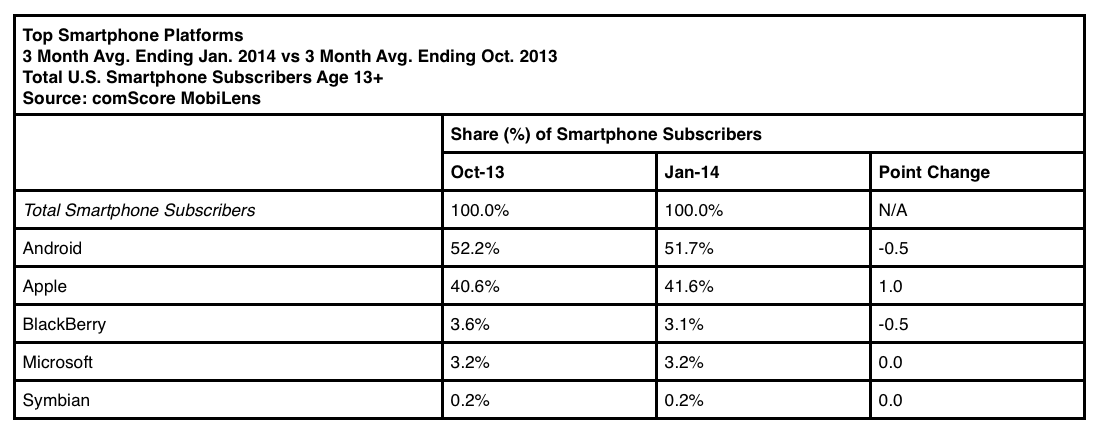
\includegraphics[width=1\textwidth]{Figuras/moviles.png}
		\rule{35em}{0.5pt}
	\caption[Mercado de los S.O. Móviles]{Presencia Actual en el Mercado de los S.O. Móviles}
	\label{fig:moviles}
\end{figure}
% Capitulo 2

\chapter{Estado del Arte} % Main chapter title

\label{EstadoDelArte} % For referencing the chapter elsewhere, use \ref{Chapter1} 

\lhead{Capítulo 2 \emph{Estado del Arte}} % This is for the header on each page - perhaps a shortened title

%----------------------------------------------------------------------------------------

Existen dos clases de aplicaciones que se analizaron: aplicaciones con localización en interiores y otras que brindan información sobre aeropuertos. Las Tablas \ref{tab:appsInteriores} y \ref{tab:appsViajes} muestran estas aplicaciones.

\definecolor{blanco}{RGB}{255,255,255}

\begin{table}[h] 
	\begin{center}
		\begin{tabular}{|p{1.8cm}|p{4.5cm}|p{1.05cm}|p{2.5cm}|p{2.5cm}|}
			\hline \rowcolor[RGB]{0,102,204} 
			\textcolor{blanco}{\bf Aplicación} &
				\textcolor{blanco}{\bf Descripción} &
					\textcolor{blanco}{\bf Precio} &
						\textcolor{blanco}{\bf Plataforma(s)} &
							\textcolor{blanco}{\bf Logotipo} \\
			\hline \rowcolor[RGB]{224,224,224} 
			\multirow{8}{0cm}{Crux} &
				Aplicación móvil que permite conocer la ubicación en interiores. Ofrece herramientas para potenciar las ventas, las visitas, la fidelidad de los clientes, la experiencia de compra y su grado de satisfacción. &
					\multirow{8}{0cm}{Gratis} &
						\multirow{8}{0cm}{Android} &
							\multirow{7}{0cm}{\raisebox{-\totalheight}{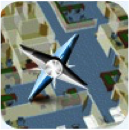
\includegraphics[width=25mm, height=25mm]{Figuras/crux.png}}} \\
      		\hline 
      		\multirow{8}{0cm}{Meridian} &
      			Guía a los viajeros paso a paso hacia el lugar que deseen visitar dentro del aeropuerto. Integra bases de datos de las tiendas en el aeropuerto, horarios de vuelos y cuentas de redes sociales. &
      				\multirow{8}{0cm}{Gratis} &
      					\multirow{8}{0cm}{iOS y Android} &
      						\multirow{7}{0cm}{\raisebox{-\totalheight}{
\includegraphics[width=25mm, height=25mm]{Figuras/meridian.png}}} \\
      		\hline 
		\end{tabular}
	\end{center}
	\caption[Aplicaciones para Localización en Interiores]{Aplicaciones para localización en Interiores} 
	\label{tab:appsInteriores}
\end{table}


\begin{table}[h] 
	\begin{center}
		\begin{tabular}{|p{1.8cm}|p{4.5cm}|p{1.05cm}|p{2.5cm}|p{2.5cm}|}
			\hline \rowcolor[RGB]{76,153,0}
			\textcolor{blanco}{\bf Aplicación} &
				\textcolor{blanco}{\bf Descripción} &
					\textcolor{blanco}{\bf Precio} &
						\textcolor{blanco}{\bf Plataforma(s)} &
							\textcolor{blanco}{\bf Logotipo} \\
			\hline \rowcolor[RGB]{224,224,224} 
			\multirow{12}{0cm}{GateGuru} &
				Recibe datos de unos 180 aeropuertos ubicados en EE.UU., Canadá, Europa y Asia, de tal forma que da a conocer el estado de vuelos. La aplicación también permite visualizar itinerarios conectándose con Tripit y Kayak. Además de obtener mapas, información sobre el clima y alquileres de coche. &
					\multirow{12}{0cm}{Gratis} &
						\multirow{12}{2.5cm}{iOS, Android y Windows Phone} &
							\multirow{11}{0cm}{\raisebox{-\totalheight}{
\includegraphics[width=25mm, height=25mm]{Figuras/gateGuru.png}}} \\
      		\hline \multirow{11}{0cm}{Kayak} &
      			Es un gran buscador que ahora ha pasado a ser también una aplicación. Con Kayak se pueden comparar ofertas de vuelo, hoteles y alquileres de coches, así como buscar tarifas de equipajes; acceder a los teléfonos de las aerolíneas y a la información de los aeropuertos. &
      				\multirow{11}{0cm}{Gratis} &
      					\multirow{11}{2.5cm}{iOS, Android, Windows Phone y Kindle Fire.} &
      						\multirow{10}{0cm}{\raisebox{-\totalheight}{
\includegraphics[width=25mm, height=25mm]{Figuras/kayak.png}}} \\
      		\hline \rowcolor[RGB]{224,224,224} 
      		\multirow{9}{0cm}{Tripit} &
      			Es un organizador de viajes que se puede usar desde el teléfono o la tableta en conexión directa con tripit.com.
Además la aplicación alerta sobre posibles retrasos de vuelos y cuenta con un despertador, muy útil si se viaja temprano. &
					\multirow{9}{1.05cm}{\$ 49 anual} &
						\multirow{9}{2.5cm}{iOS, Android, Blackberry y Windows Phone.} &
							\multirow{8}{0cm}{\raisebox{-\totalheight}{
\includegraphics[width=25mm, height=25mm]{Figuras/tripit.png}}} \\
      		\hline
		\end{tabular}
	\end{center}
	\caption[Aplicaciones con Información de Viajes]{Aplicaciones con Información de Viajes} 
	\label{tab:appsViajes}
\end{table}

\newpage
A continuación se muestra una recopilación de las publicaciones que se han desarrollado sobre la localización en interiores.

\begin{table}[h] 
	\begin{center}
		\begin{tabular}{|p{4cm}|p{4.5cm}|p{4.5cm}|}
			\hline \rowcolor[RGB]{0,0,0} 
			\textcolor{blanco}{\bf Artículo}	 &
				\textcolor{blanco}{\bf Autores} &
					\textcolor{blanco}{\bf Resumen} \\
			\hline \rowcolor[RGB]{224,224,224} 
			\multirow{8}{4cm}{ILS (Indoor Location Systems) Sistemas de Localización en Interiores} &
				\multirow{8}{4.5cm}{Raúl Sánchez Vítores} &
					Este trabajo presenta los problemas existentes de la localización en interiores para después presentar una clasificación de los sistemas ILS y las distintas soluciones técnicas que se han desarrollado. \\
      		\hline \multirow{9}{4cm}{Uso del campo magnético de la tierra para localizar a las personas en interiores} &
      			\multirow{9}{4.5cm}{Carlos Eric Galván Tejada \newline
				Juan Pablo García Vázquez \newline
				Jorge Isaac Galván Tejada} &
      				Este trabajo explica las técnicas que se emplean para localizar en interiores utilizando el campo magnético y menciona las ventajas que se tienen a comparación de otras formas de realizar la localización en interiores. \\
      		\hline 
		\end{tabular}
	\end{center}
	\caption[Publicaciones sobre Localización en Interiores]{Publicaciones sobre Localización en Interiores} 
	\label{tab:publicacionesInteriores}
\end{table}



%----------------------------------------------------------------------------------------
% Capitulo 3

\chapter{Marco Teórico} % Main chapter title

\label{MarcoTeorico} % For referencing the chapter elsewhere, use \ref{Chapter1} 

\lhead{Capítulo 3 \emph{Marco Teórico}} % This is for the header on each page - perhaps a shortened title

%----------------------------------------------------------------------------------------

En este capítulo se introducen los conceptos necesarios que son indispensables conocer para el desarrollo del proyecto. Se considera como necesario todo aquel conocimiento que intervenga en el proceso de construcción del sistema y que sea crítico para el cumplimiento de los objetivos establecidos.

%----------------------------------------------------------------------------------------

\section{Aplicación Móvil}

Una aplicación móvil, más comúnmente conocida como una aplicación, es un tipo de software de aplicación diseñado para ejecutarse en un dispositivo móvil, como un ordenador smartphone o tablet. Las aplicaciones móviles sirven con frecuencia para proporcionar a los usuarios servicios similares a los que se accede en las PC. \cite{queParaApps}

Las aplicaciones móviles están diseñadas con la consideración de las exigencias y limitaciones de los dispositivos y también para aprovechar las capacidades especializadas que tienen.

Cabe mencionar que existen 3 tipos de aplicaciones móviles, las cuales pueden ser: 

\begin{itemize}
	\item \textbf{Nativas: }Diseñadas para exclusivamente correr en un sistema operativo específico.
	\item \textbf{Web: }Estas corren por medio de los navegadores propios de cada teléfono y  están configuradas para que puedan verse en un dispositivo móvil.
	\item \textbf{Híbridas: }Este tipo de aplicaciones resultan de la combinación de la anteriores como por ejemplo Facebook  que se descarga como una aplicación nativa pero se tiene que estar actualizando constantemente y que además puede verse de manera web en caso de no tener la aplicación instalada.\cite{tiposApps}
\end{itemize}

\section{Cómputo Móvil}

Sistema de computación en donde el usuario puede estar en movimiento, esto consiste en fabricar computadoras suficientemente pequeñas para ser fácilmente transportadas. Se tiene la necesidad de reemplazar los cables de conexión por una tecnología inalámbrica.

Este tipo de tecnología no solo representa una oportunidad de avance científico o computacional sino de implementar nuevas posibilidades de negocios como:

\begin{itemize}
	\item Aplicaciones financieras
	\item Gerencia de inventario
	\item Gerencias de servicios de campo
	\item Localización de productos
\end{itemize}

\subsection{Características de la Computación Móvil}

\begin{itemize}
	\item \textbf{Movilidad: }Implica la portabilidad basada en el hecho de que los usuarios llevan un dispositivo móvil a todas las partes a donde se dirigen, por lo tanto, los usuarios pueden iniciar el contacto en tiempo real con otros sistemas dondequiera que se encuentren.
	\item \textbf{Amplio alcance: }Es la característica que describe la accesibilidad de las personas, que se pueden localizar en cualquier momento.
	\item \textbf{Ubicuidad: }Se refiere al atributo de estar disponible en cualquier lugar en cualquier momento. Un terminal móvil en la forma de un teléfono inteligente o un PDA ofrece la ubicuidad.
	\item \textbf{Comodidad: }Es muy conveniente para los usuarios operar en el entorno inalámbrico, todo lo que necesitan es un dispositivo de Internet móvil, como un teléfono inteligente.
	\item \textbf{Conectividad instantánea: }Los dispositivos móviles permiten a los usuarios conectarse de manera sencilla y rápida a la Internet e intranets, de otros dispositivos móviles y bases de datos.
	\item \textbf{Personalización: }Se refiere a la personalización de la información para los consumidores individuales.
    	\item \textbf{Localización de productos y servicios: }Conocer la ubicación física de los usuarios en cualquier momento es clave para ofrecer productos y servicios.
\end{itemize}
\section{Cómputo Ubicuo}

Es la integración de la informática en el entorno de la persona, de forma que los ordenadores no se perciban como objetos extraños.

Utilización de muchos dispositivos de computación que están presentes en los entornos físicos: casa, oficina y otros.

\begin{figure}[h!]
	\centering
		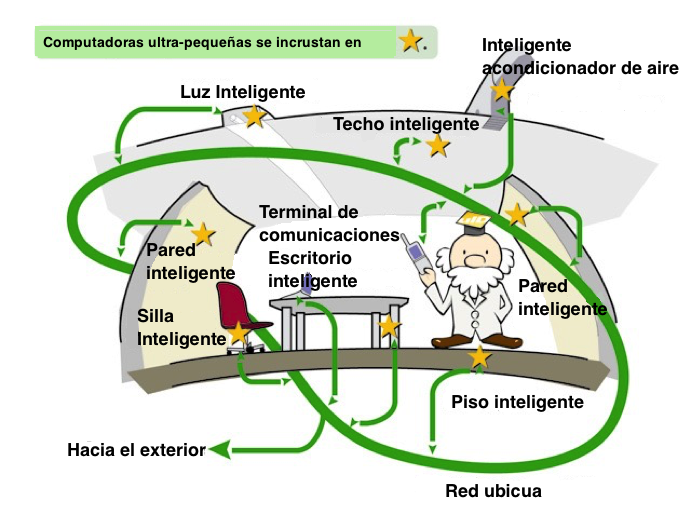
\includegraphics[width=0.8\textwidth]{Figuras/ubicuo.png}
		\rule{35em}{0.5pt}
	\caption[Integración de dispositivos inteligentes en el ambiente]{Integración de dispositivos inteligentes en el ambiente \cite{ubicuo}}
	\label{fig:ubicuo}
\end{figure}

\section{GPS}

\newcommand{\grad}{\hspace{-2mm}$\phantom{a}^{\circ}$}

GPS es la abreviatura de Global Positioning System ó Sistema de Posicionamiento Global en español. Es un sistema de radionavegación basado en satélites desarrollado y controlado por el Departamento de Defensa de Estados Unidos de América que permite a cualquier usuario saber su localización, velocidad y altura, las 24 horas del día, bajo cualquier condición atmosférica y en cualquier punto del globo terrestre. 

Después de la segunda guerra mundial, el Departamento de Defensa de Estados Unidos de América se empeñó en encontrar una solución para el problema del posicionamiento preciso y absoluto. Pasaron varios proyectos y experiencias durante los siguientes 25 años, incluyendo Loran, Transit, etc. Todos permitían determinar la posición pero eran limitados en precisión o funcionalidad. En el comienzo de la década de 70, un nuevo proyecto fue propuesto, el GPS. 

El GPS tiene tres componentes: el espacial, el de control y el de usuario.

El componente espacial está constituido por una constelación de 24 satélites en órbita terrestre aproximadamente a 20200 km, distribuidos en 6 planos orbitales. Estos planos están separados entre sí por aproximadamente 60\grad  en longitud y tienen inclinaciones próximas a los 55\grad  en relación al plano ecuatorial terrestre. Fue concebido de manera que existan como mínimo 4 satélites visibles por encima del horizonte en cualquier punto de la superficie y en cualquier altura.

El componente de control está constituido por 5 estaciones de rastreo distribuidas a lo largo del globo y una estación de control principal (MCS- Master Control Station). Este componente rastrea los satélites, actualiza sus posiciones orbitales y calibra y sincroniza sus relojes. Otra función importante es determinar las órbitas de cada satélite y prever su trayectoria durante las 24 horas siguientes. Esta información es enviada a cada satélite para después ser transmitida por este, informando al receptor local donde es posible encontrar el satélite. 

El componente del usuario incluye todos aquellos que usan un receptor GPS para recibir y convertir la señal GPS en posición, velocidad y tiempo. Incluye además todos los elementos necesarios en este proceso, como las antenas y el software de procesamiento. 

\subsection{Funcionamiento GPS}

Los fundamentos básicos del GPS se basan en la determinación de la distancia entre un punto: el receptor, a otros de referencia: los satélites. Sabiendo la distancia que nos separa de 3 puntos podemos determinar nuestra posición relativa a esos mismos 3 puntos a través de la intersección de 3 circunferencias cuyos radios son las distancias medidas entre el receptor y los satélites. En la realidad, son necesarios como mínimo 4 satélites para determinar nuestra posición correctamente. 

Cada satélite transmite una señal que es recibida por el receptor, éste, por su parte mide el tiempo que las señales tardan a llegar hasta él. Multiplicando el tiempo medido por la velocidad de la señal (la velocidad de la luz), obtenemos la distancia receptor-satélite, (Distancia = Velocidad X Tiempo).

Sin embargo el posicionamiento satelital no es así de simple. Obtener la medición precisa de la distancia no es tarea fácil.

La distancia puede ser determinada a través de los códigos modulados en la onda enviada por el satélite  (códigos C/A y P), o por el análisis de la onda portadora. Estos códigos son complicados. El receptor fue preparado de modo que solamente descifre esos códigos y ninguno más, de este modo él está inmune a interferencias generadas por fuentes naturales o intencionales. Esta es una de las razones para la complejidad de los códigos.  \cite{GPS}
\section{ILS (Indoor Location Systems) Sistemas de Localización en Interiores}

La problemática de la localización en interiores ha sido objeto de un intenso estudio e investigación durante los últimos años. Hasta ahora, ninguna de las soluciones propuestas ha conseguido el éxito que han alcanzado los sistemas de localización y navegación análogos empleados en exteriores, sobre todo el popular GPS. Las razones de este cierto fracaso han sido tanto técnicas como sobre todo económicas: técnicas porque la localización en interiores plantea retos tecnológicos muy superiores a los de la localización en espacios abiertos y económicas porque la mayor parte de los sistemas propuestos utilizan gran cantidad de infraestructura fija (sensores, puntos de control, estaciones base, etc.), lo que hace aumentar mucho el costo.

\subsection{Clasificación de los sistemas ILS}

Por una parte podemos distinguir los sistemas \textbf{basados en tags o etiquetas}, en los cuales el equipo sólo es capaz de detectar y por lo tanto localizar, a aquellos elementos que porten un dispositivo conocido como tag, y por consiguiente al elemento etiquetado.

Por el contrario, los que no precisan de tags son sistemas que sí que son capaces de reconocer y detectar al elemento a seguir.

La ventaja de esta clase de sistemas es que permiten la localización y seguimiento de cualquier elemento, por lo que son de aplicación universal y además son mucho más seguros. No obstante, sus prestaciones son todavía muy limitadas y no son eficaces, excepto en ambientes muy controlados.

Además, están los basados en la \textbf{detección de presencia por un sensor} localizado y de ubicación fija y conocida, llamado punto de control. Una vez detectado el elemento e identificado, la localización del mismo queda acotada a las proximidades del sensor que lo ha identificado. Por consiguiente, la localización se basa en los criterios de presencia y proximidad, dependiendo la precisión del sistema del número de puntos de control desplegados.

También están los sistemas basados en el \textbf{cálculo efectivo de la posición del elemento mediante técnicas de triangulación}, conociendo además otros parámetros como la medida del retardo de propagación o la fuerza de la señal recibida, la ventaja de esta clase de sistemas radica en que alcanzan una gran precisión (en algunos casos del orden de centímetros), y el principal inconveniente se encuentra en el alto costo de la infraestructura a instalar y la complejidad tecnológica.

Por último, citar los equipos basados en el \textbf{análisis del escenario}, que son de mayor complejidad computacional, tratándose de sistemas que analizan determinadas propiedades del escenario en el que se pretende ubicar el elemento para inferir de ellas la posición del mismo. \cite{ILS}

\subsection{Distintas soluciones técnicas}

\subsubsection{Identificación por radiofrecuencia}

Como su nombre indica, son propiamente sistemas de identificación, no de localización, aunque también pueden utilizarse para esta función. Aunque existen multitud de criterios para clasificar los sistemas de RFID, se distinguen dos clases fundamentales en función del tipo de tags que se empleen: pasivos (sin batería) o activos (con batería). Otros criterios de clasificación habituales son la frecuencia de trabajo, si los tags son de sólo lectura o de lectura y escritura, etc. 

Aquí simplemente vamos a presentar las principales características de los tags pasivos y activos. 

Un tag pasivo consiste en una unidad de procesamiento, un transmisor de RF (radiofrecuencia)
y una antena, la cual actúa tanto para la transmisión de la información contenida en el tag (un código de identificación
numérico) como para la alimentación del tag a través de un bucle de inducción a partir de la emisión electromagnética del lector. Cuando el tag cae bajo el radio de acción del lector, el cual emite una señal electromagnética a una determinada frecuencia, el tag carga su batería y transmite su número de identificación, normalmente a una frecuencia distinta. Las principales ventajas de esta clase de tags son su bajo coste, pequeño tamaño y gran duración. En contrapartida el alcance es muy reducido, en torno a un metro en el mejor de los casos, aunque desde hace tiempo se lleva anunciando la salida al mercado de tags pasivos en la banda de UHF (868 MHz en Europa) con alcances de 10 m ó más, pero éstos no acaban de aparecer. La localización se basa en el criterio de proximidad, y la precisión depende del número de puntos de control instalados y la correcta elección de los emplazamientos (por ejemplo, en los puntos de paso forzoso, como en las puertas). En esta clase de sistemas, el coste más elevado por unidad es el de los lectores, aunque en términos globales entre el 50 y el 70% de la inversión total corresponde a los tags. 

Por otra parte están los tags activos, que se caracterizan por disponer de una batería propia que les proporciona la energía suficiente para radiar su código de identificación con mucha mayor potencia que en el caso de los tags pasivos. En consecuencia, el alcance resulta mucho mayor (en torno a los 30 m). Como contrapartida, el coste de los tags activos es mucho mayor, así como su tamaño. El ciclo de vida del tag es el de la batería, que se sitúa alrededor de los 5 años, aunque esto depende de lo intensivo que sea su uso. Los tags activos son apropiados tanto para la implementación de sistemas ILS basados en proximidad (puntos de control), como para sistemas que hagan uso de técnicas de triangulación. 

\subsubsection{Infrarrojos}

Fue la primera tecnología empleada para el desarrollo de sistemas de localización en interiores. Se utilizan tags que emiten radiación infrarroja en modo difuso, es decir, de forma radial, no en modo punto a punto como es habitual en los sistemas IR empleados en comunicaciones. Se trata de un sistema de detección más que de localización, ya que la posición del elemento etiquetado con el tag IR se infiere de la posición fija y conocida de los sensores que detectan al tag. 

La principal limitación de esta alternativa tecnológica es que la radiación infrarroja no atraviesa las paredes, por lo que hay que instalar sensores en cada una de las habitaciones. Además, debido a que la emisión es directiva por el efecto pantalla del cuerpo del portador del tag, es conveniente instalar más de un sensor por localización para asegurar que la detección se produzca correctamente, lo cual hace aumentar mucho el coste. No obstante, con este sistema se obtiene la gran ventaja de conseguir evitar interferencias y falsas detecciones de otros sensores, como sucede en RF. 

\subsubsection{Pinpoint 3D-ID de RF technologies}

PinPoint es un sistema que se basa en estaciones base y tags activos de RFID propietarios de tecnología L3RF (Low range, Long life, Low cost), y requiere el despliegue de una red ad hoc (única para este propósito). 

Los tags se activan al recibir desde una estación base o un controlador de celda (que controla hasta un máximo de 16 antenas), una señal de radio a la frecuencia de 2,4 GHz y responden a intervalos definidos, a la frecuencia de 5,8 GHz con señales que incluyen información de identificación del tag. Observando el retardo de la respuesta del tag en cada estación base o antena, el controlador de celda es capaz de calcular la posición del tag. 

El mayor inconveniente es que cada antena del sistema tiene un área de cobertura muy limitada, las antenas son muy directivas, por lo que es necesario un gran despliegue de infraestructura para cubrir un área, siendo por tanto una solución muy costosa más orientada a naves industriales y almacenes de gran tamaño que a edificios con numerosos tabiques y habitaciones. 

\subsubsection{Radar}

Sistema presentado por Microsoft en marzo del 2000, que hace uso de la tecnología IEEE 802.11. Se basa en las mediciones que las estaciones base de una red WLAN (Wireless LAN) hacen de la potencia y de la relación señal a ruido de las emisiones transmitidas por los dispositivos inalámbricos que se conectan a la red. Una serie de algoritmos permiten estimar la localización de un elemento con una precisión de 3 a 4 m en el 50\% de las ocasiones. Microsoft ha desarrollado dos versiones de la herramienta, una empleando análisis del escenario y otra que emplea triangulación por distancias para el cálculo de la posición. 

La ventaja de este sistema es que requiere, si lo comparamos con otros sistemas, relativamente poca infraestructura. También es interesante que se pueda apoyar sobre redes WLAN ya instaladas para otros propósitos. Como desventajas hay que señalar que sólo pueden ser localizados elementos con capacidad de conexión WLAN y que la aplicación del sistema en edificios con varias plantas, genera problemas de difícil solución debido a que las ondas de radio también pueden atravesar suelos y techos. Así pues, si las señales de un mismo tag son captadas por estaciones base instaladas en plantas distintas, y en función de la potencia con que se reciban, el sistema puede llegar a ubicar al tag en un piso que no le corresponde. Hay que señalar, por otra parte, que las tarjetas WLAN no son baratas y tienen importantes consumos de energía, por lo que difícilmente pueden acomodarse a tags de reducido peso y tamaño. 

\subsubsection{Ultrasonidos}

Se trata de soluciones que están también basadas en tags o etiquetas para los elementos a controlar, pero en este caso estos tags emiten o reciben ultrasonidos. El sistema más representativo es el Bat de AT\&T Laboratories. Los tags cuentan con un transceptor radio (banda de 433 MHz), una lógica de control que contiene un identificador único de 48 bits y un emisor de ultrasonidos. La infraestructura se compone de sensores de ultrasonidos, estaciones base de RF y un sistema central de gestión, formando los sensores o receptores una malla en puntos conocidos del techo. Una estación base transmite periódicamente un mensaje que contiene el identificador del tag que desea activar y al recibir el mensaje con su identidad, el tag aludido se despierta y emite un pulso de muy corta duración. Además, se resetea el reloj de los sensores del área de influencia, los cuales comienzan a contar el tiempo que transcurre hasta que reciben la señal del tag Bat. A partir de este retardo y de la velocidad de propagación del sonido en el aire, se calcula de forma inmediata la distancia al sensor. Cabe destacar que con las distancias del tag a varios sensores (mínimo tres), puede conocerse la posición del tag en 3 dimensiones. Este sistema es capaz de detectar la posición de los tags con un error máximo de 3 cm en un 95\% de las medidas. Cada estación base puede activar simultáneamente un número máximo de 3 tags, con una frecuencia de refresco de 50 veces por segundo. El tiempo de vida de la batería del tag es de 15 meses. El sistema Bat no se comercializa en la actualidad debido al alto coste de la infraestructura, que se espera poder reducir en posteriores versiones del sistema. Otro de los retos que pretenden acometer los investigadores de AT\&T es la sustitución de las comunicaciones RF entre estaciones base y tags por IR para evitar la complejidad del trabajo multifrecuencia en estaciones base próximas. En cualquier caso, se trata de una tecnología poco madura y bastante elevada en precio, encontrándose todavía lejos de ser comercializada. 

\subsubsection{Visión Artificial}

Estos sistemas hacen uso de la información recogida por cámaras y utilizan técnicas de procesamiento de imágenes para la identificación y seguimiento de objetos. Estos sistemas de visión empleados en identificación y localización pueden trabajar tanto con marcadores visuales (tags) como sin ellos. 

\subsubsection{Zigbee}

Iniciado por Philips, Honeywell, Invensys y seguido por Motorota, Mitsubishi y hasta 25 empresas para crear un sistema estándar de comunicaciones inalámbrico y bidireccional, para usarlo dentro de dispositivos de domótica, automatización de edificios (inmótica), control industrial, periféricos de PC, sensores médicos e identificación y localización. La idea de ponerle el nombre ZigBee vino de una colmena de abejas pululando alrededor de su panal y comunicándose entre ellas.
Los miembros de esta alianza justifican el desarrollo de este estándar para cubrir el vacío que se produce por debajo del Bluetooth. Puede transmitir con un simple protocolo de 20 KB/s trabajando a una frecuencia de 2,4 GHz (banda libre ISM) u 868 MHz (Europa) o 915 MHz (EEUU), con bajo consumo (“transceiver” ZigBee dormido la mayor parte del tiempo), rangos entre 10 y 75 metros y soporte de hasta 255 nodos. 

\subsubsection{Campo Magnético}

Los sistemas de localización basados en el campo magnético de la tierra pueden ser agrupados principalmente en dos categorías, aquellos que requieren de una fase pasiva más extensa y detallada, refiriéndose a una recolección de información meticulosa dividiendo el área en superficies pequeñas de igual tamaño y obtener para cada una de esas pequeñas superficies su lectura del campo magnético \cite{usoCampoMagnetico}, como lo podemos visualizar en la Figura \ref{fig:ejPasiva}.

\begin{figure}[htbp]
	\centering
		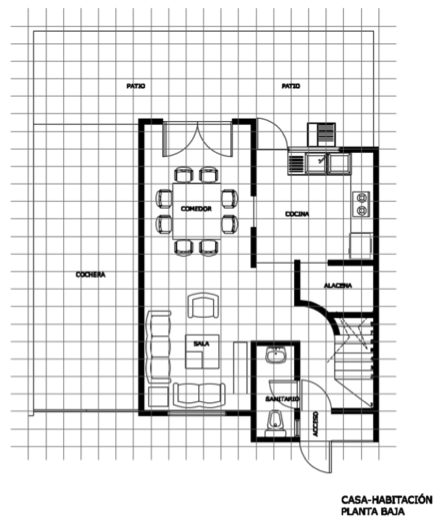
\includegraphics{Figuras/ejPasiva.png}
		\rule{35em}{0.5pt}
	\caption[División de una casa habitación para la recolección de información en la fase pasiva]{Ejemplo de división de una casa habitación para la recolección de información en la fase pasiva}
	\label{fig:ejPasiva}
\end{figure}

Por otro lado, se tiene el enfoque siguiendo al líder (follow the leader), en el cual la fase pasiva es mucho más sencilla, ya que solamente consta de recolectar información dentro de la habitación generando un perímetro o recorrido predefinido que en la fase activa puede ser reconocido y así obtener la localización, enfoque representado en la Figura \ref{fig:ejSigLider}.

 \begin{figure}[htbp]
	\centering
		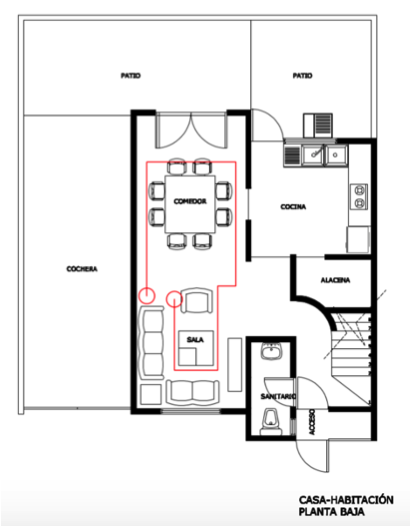
\includegraphics{Figuras/ejSigLider.png}
		\rule{35em}{0.5pt}
	\caption[Perímetro requerido en el enfoque siguiendo al líder  para reconocer una habitación]{Ejemplo de perímetro requerido en el enfoque siguiendo al líder  para reconocer una habitación}
	\label{fig:ejSigLider}
\end{figure}
\section{Sistema Operativo Móvil Android}

Android es un sistema operativo y una plataforma software, basado en Linux, que junto con aplicaciones middleware está enfocado para ser utilizado en dispositivos móviles como teléfonos inteligentes, tabletas, google TV y otros dispositivos. Android permite programar en un entorno de trabajo (framework) de Java, lo que nos asegura que podrán ser ejecutadas en cualquier tipo de CPU, tanto presente como futuro. Aplicaciones sobre una máquina virtual Dalvik (una variación de la máquina de Java con compilación en tiempo de ejecución creada por Google optimizada para dispositivos móviles). Además, lo que le diferencia de otros sistemas operativos, es que cualquier persona que sepa programar puede crear nuevas aplicaciones, widgets o incluso, modificar el propio sistema operativo, dado que Android es de código libre. \cite{Android}

\begin{figure}[htbp]
	\centering
		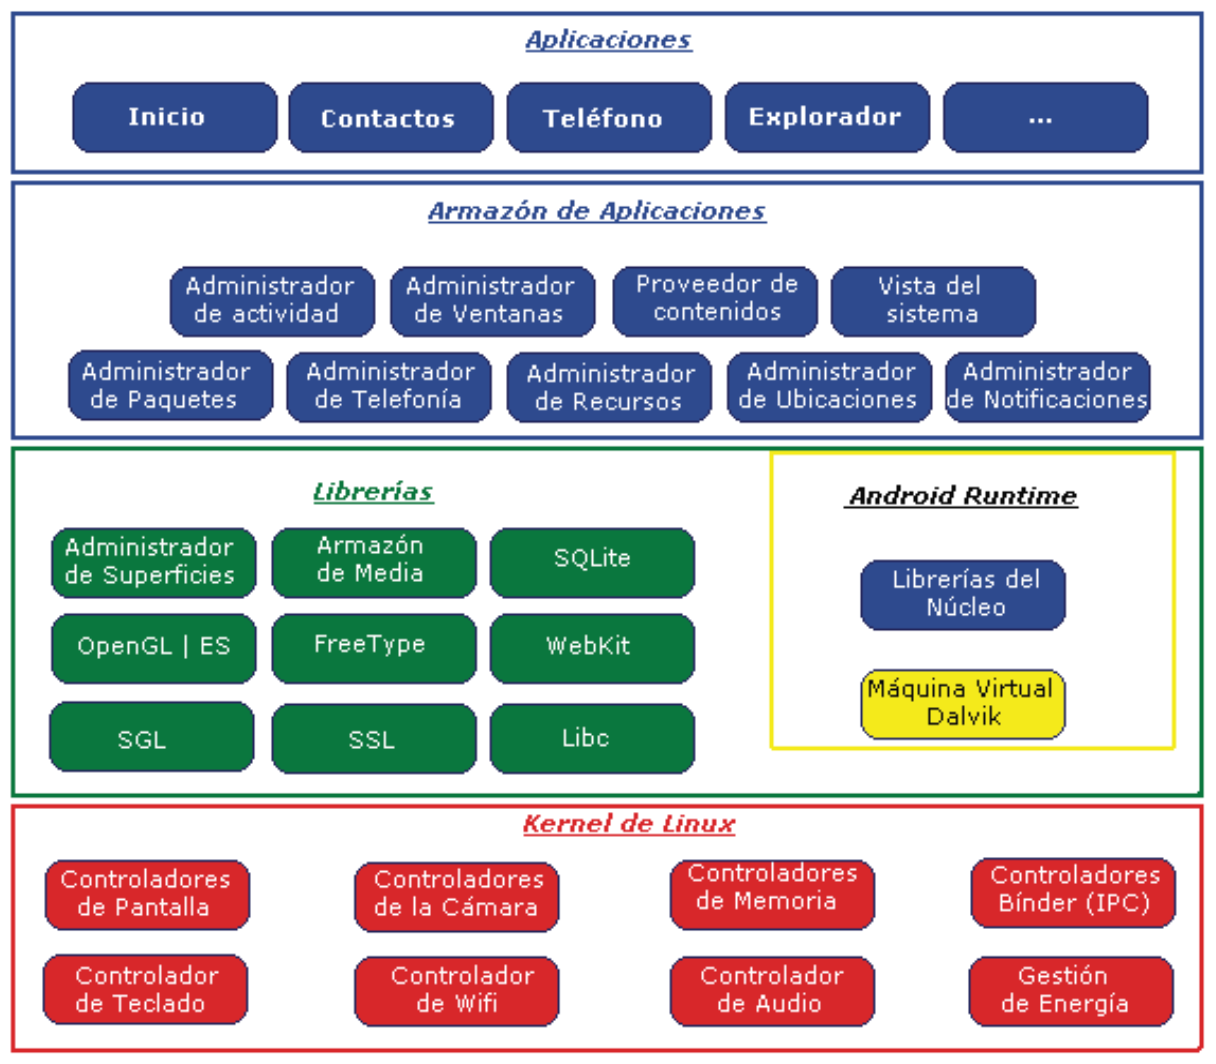
\includegraphics[width=1\textwidth]{Figuras/capasAndroid.png}
		\rule{30em}{0.5pt}
	\caption[Sistema de capas de Android]{Sistema de capas de Android}
	\label{fig:capasAndroid}
\end{figure}

En la Figura \ref{fig:capasAndroid} se distinguen claramente cada una de las capas: la que forma parte del propio Kernel de Linux, donde Android puede acceder a diferentes controladores, las librerías creadas para el desarrollo de aplicaciones Android, la siguiente capa que organiza los diferentes administradores de recursos, y por último, la capa de las aplicaciones a las que tiene acceso.

\begin{itemize}
	\item \textbf{Arquitectura basada en componentes}
	\begin{itemize}
		\item El diseño de la interfaz de usuario se hace en xml, lo que permite que una misma aplicación se ejecute en un dispositivo móvil de pantalla reducida o en un TV.
	\end{itemize}
	\item \textbf{Filosofía de dispositivo siempre conectado a Internet}
	\begin{itemize}
		\item Servicios incorporados basados en Web.
		\item Localización basada tanta en GPS como en redes, bases de datos con SQL, navegadora, multimedia.
	\end{itemize}
	\item \textbf{Aceptable nivel de seguridad}
	\begin{itemize}
		\item Los programas se encuentran aislados unos de otros gracias al concepto de ejecución dentro de una caja que hereda de Linux.
		\item Cada aplicación dispone de una serie de permisos que limitan su rango de actuación (servicios de localización, acceso a Internet, etc.)
	\end{itemize}
	\item \textbf{Calidad de gráficos y sonido}
	\begin{itemize}
		\item Gráficos en 3 dimensiones basados en OpenGL.
		\item Gráficos vectoriales suavizados.
		\item Animaciones inspiradas en Flash.
		\item Incorpora codecs estándar más comunes de audio y vídeo, incluyendo H.264 (AVC), MP3, AAC, etc.
	\end{itemize}
\end{itemize}

\subsection{Características de Android}

\begin{itemize}
	\item \textbf{Acceso a Hardware, incluyendo Cámara, GPS y Sensores: }Android incluye API’s que permite simplificar el desarrollo sin importar el hardware sobre el que se está trabajando. Esto asegura que no necesitamos crear implementaciones específicas para distintos dispositivos, así que podemos crear aplicaciones que deben trabajar según lo esperado en cualquier dispositivo que tenga una versión compatible de Android.
	\item \textbf{Transferencia de Datos con Wi-Fi, BlueTooth y NFC: } Android ofrece soporte muy completo para transferir datos entre dispositivos, incluyendo Bluetooth, Wi-Fi y Android Beam. Estas tecnologías permiten compartir datos entre dispositivos, dependiendo del hardware disponible en el dispositivo utilizado.
	\item \textbf{Mapas y Geolocalización: }El manejo de mapas embebido con el que cuenta Android permite crear aplicaciones que de manera programática pueden manipular los mapas de Google Maps. Además, la integración de un GPS y los servicios de localización de Google para determinar la ubicación actual del dispositivo, permite combinar posicionamiento con mapas.
	\item \textbf{Servicios en Segundo Plano (Background Services): }Android soporta aplicaciones y servicios diseñados para ser ejecutados en segundo plano, mientras nuestra aplicación no está activa, debido a que solamente una aplicación puede estar visible a la vez. 
	\item \textbf{Base de Datos SQLite: }El almacenamiento y la recuperación de información de manera rápida y eficiente es básica para dispositivos con capacidad limitada. Android utiliza SQLite para cumplir con este objetivo. Las aplicaciones móviles pueden aprovechar esta base de datos relacional para almacenar y recuperar información de manera segura y eficiente.
	\item \textbf{Compartición de Datos y Comunicación entre Aplicaciones: }Android incluye técnicas para compartir información entre las distintas aplicaciones, tales como: Intents y Content Providers.
	\item \textbf{ Soporte para gráficos 2D y 3D: }Android provee librerías gráficas para dibujos 2D y 3D con OpenGL. Además, Android provee soporte para imágenes, video, audio, incluyendo video en formato mpeg4.
	\item \textbf{Optimización de Memoria y Administración de Procesos: }Android utiliza su propia maquina virtual para la administración de la memoria. Android asegura que una aplicación responda en un tiempo determinado, de lo contrario la detiene y la puede eliminar en caso de ser necesario, con el objetivo de liberar recursos. De esta manera Android controla el ciclo de vida de las aplicaciones en un ambiente enfocado en hacer más eficiente el uso de memoria de los dispositivos. \cite{presentacionAndroid}
\end{itemize}

% Capitulo 4

\chapter{Marco Metodológico} % Main chapter title

\label{MarcoMetodologico} % For referencing the chapter elsewhere, use \ref{Chapter1} 

\lhead{Capítulo 4 \emph{Marco Metodológico}} % This is for the header on each page - perhaps a shortened title

%----------------------------------------------------------------------------------------

Para poder llegar a la construcción final de un producto de software existen una gran variedad de modelos definidos por la ingeniería de software, los cuales son aplicables dependiendo a las características del proyecto a desarrollar, así como cada uno optimiza el desarrollo del mismo dependiendo de su definición. 

Las metodologías ágiles nos permiten aplicar modelos en los que se tiene una retroalimentación del cliente considerándolo como parte del equipo de desarrollo, como lo es Mobile-D.

La metodología Mobile-D se desarrolló junto con un proyecto finlandés en el 2004.

Fue realizado, principalmente, por investigadores de la VTT (Instituto de Investigación Finlandés.)

El objetivo es conseguir ciclos de desarrollos muy rápidos en equipos muy pequeños (de no más de diez desarrolladores) trabajando en un mismo espacio físico. Según este método, trabajando de esa manera se deben conseguir productos totalmente funcionales en menos de diez semanas.

Mobile-D es una metodología para el desarrollo ágil de software, que no solamente está orientado al desarrollo de aplicaciones móviles, también se puede usar en aplicaciones de seguridad, financieras, de logística y de simulación.
Mobile-D se basa en la Programación Extrema (XP) para la implementación, Crystal Methodologies para la escalabilidad y en el Proceso Unificado de Desarrollo (RUP) para la cobertura del ciclo de vida.

%----------------------------------------------------------------------------------------

\begin{figure}[htbp]
	\centering
		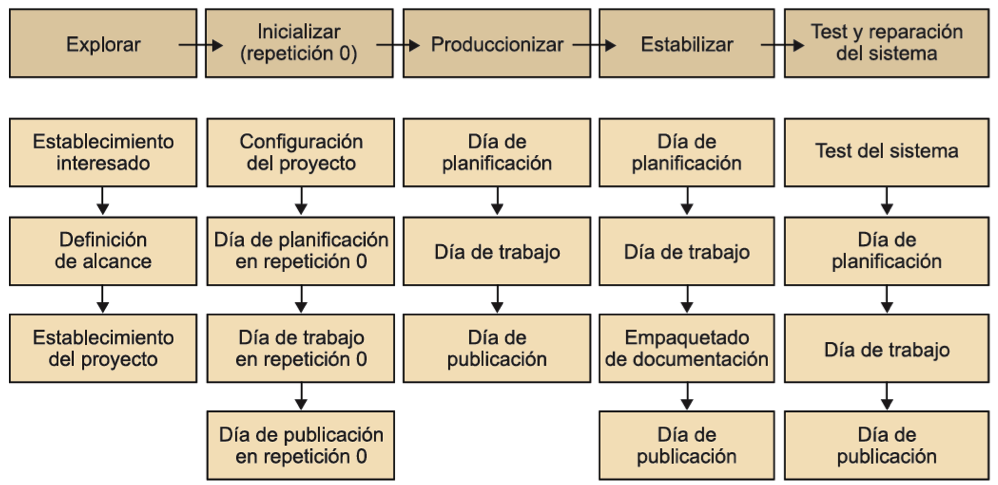
\includegraphics[width=1\textwidth]{Figuras/cicloDesarrollo.png}
		\rule{30em}{0.5pt}
	\caption[Ciclo de desarrollo de Mobile-D]{Ciclo de desarrollo de Mobile-D}
	\label{fig:cicloDesarrollo}
\end{figure}

\begin{itemize}
	\item \textbf{Exploración: }El propósito de la fase de exploración es planear y establecer el proyecto. Esta fase es importante para establecer las bases para la arquitectura del producto, la elección del entorno, y la implementación del sistema.
	\item \textbf{Inicialización: }El propósito de la fase de inicialización es posibilitar el éxito de las siguientes fases del proyecto preparando y verificando todos los problemas críticos del desarrollo, de manera que todos ellos sean corregidos con prontitud en el final de la fase de  aplicación de los requisitos. Además se preparan todos los recursos físicos, tecnológicos y de comunicaciones para las actividades de producción. 
	\item \textbf{Producción: }La fase de producción tiene como propósito implementar la funcionalidad requerida en el producto aplicando un ciclo de desarrollo iterativo e incremental. El desarrollo basado en pruebas es utilizado para implementar las funcionalidades.
	\item \textbf{Estabilización: }El propósito de la fase de estabilización es asegurar la calidad de la implementación del proyecto.
	\item \textbf{Pruebas del sistema: }El propósito de la fase de pruebas del sistema es comprobar si el producto implementa las funcionalidades requeridas correctamente, y corregir los errores encontrados.
\end{itemize}

Al analizar el método de desarrollo de software antes mencionado concluimos que es el adecuado para poder aplicarlo a nuestro sistema ya que necesitamos realizar iteraciones sobre un prototipo inicial y sobre ese trabajar para poder refinarlo hasta llegar al sistema final, es decir tendremos un avance paulatino en los requerimientos y desarrollo del mismo. \cite{MobileD} \cite{desDispositivos}
% Capitulo 5

\chapter{Análisis General} % Main chapter title

\label{AnalisisGeneral} % For referencing the chapter elsewhere, use \ref{Chapter1} 

\lhead{Capítulo 5 \emph{Análisis General}} % This is for the header on each page - perhaps a shortened title

El análisis es una etapa del desarrollo de software que tiene como finalidad ayudar al desarrollador a entender los deseos del cliente, delimitar la funcionalidad del sistema y analizar la factibilidad del mismo, para poder brindar una solución total al problema presentado.

\section{Estudio de Factibilidad}

\newcommand{\tabitem}{~~\llap{\textbullet}~~}

El estudio de factibilidad sirve para estimar los recursos necesarios para el desarrollo del proyecto, el éxito de la implementación está determinado por el grado de factibilidad que se presente en tres aspectos a evaluar: técnico, económico y operativo.

\subsection{Factibilidad Técnica}

La factibilidad técnica consiste en realizar una evaluación de la tecnología con la que cuenta el equipo de trabajo, en éste estudio se muestra la información recolectada sobre los componentes técnicos con los que se cuenta y la posibilidad de hacer uso de los mismos en el desarrollo e implementación del sistema propuesto y de ser necesario, los requisitos tecnológicos que deben ser adquiridos para el desarrollo y puesta en marcha del sistema. 

De acuerdo a los requisitos del sistema se evaluaron sus componentes bajo dos enfoques: hardware y software. 

\subsubsection{Hardware}

Respecto al hardware, se requieren equipos de cómputo para: desarrollar la aplicación móvil, alojar la aplicación Web de administración y tener el servicio Web funcionando. También es necesario un teléfono inteligente que cuente con los sensores necesarios para la localización en interiores. 

El equipo de trabajo cuenta con las computadoras personales para el desarrollo de la aplicación móvil, las cuales se detallan en la Tabla \ref{tab:hardware}.

\begin{table}[h]
	\begin{center}
		\begin{tabular}{|c|c|}
			\hline \rowcolor[RGB]{51,153,255}
			\textcolor{blanco}{\bf Recurso} &
				\textcolor{blanco}{\bf Características} \\
			\hline 
			\multirow{1}{2.8cm}{Laptop Lenovo} &
				{\parbox{0.5\textwidth}{
					\begin{itemize}
                			\item Procesador Intel Core i3 2.2 GHz
		               	\item 4 GB memoria RAM DDR3
                			\item 520 GB de disco duro
                			\item Sistema Operativo Windows 7 de 64 bits
           			\end{itemize} }} \\
      		\hline \rowcolor[RGB]{240,248,255} 
      		\multirow{1}{2.8cm}{MacBook Pro} &
      				{\parbox{0.5\textwidth}{
					\begin{itemize}
                			\item Procesador Intel Core i7 2.3 GHz
		               	\item 8 GB memoria RAM
                			\item 250 GB de almacenamiento en flash
                			\item Sistema Operativo OS X 10.10.1
           			\end{itemize} }} \\
      		\hline 
		\end{tabular}
	\end{center}
	\caption[Recursos de Hardware del Equipo]{Recursos de Hardware del Equipo} 
	\label{tab:hardware}
\end{table}

Debido a la naturaleza del sistema a desarrollar, se requiere de ciertos dispositivos móviles con las características necesarias para poder implementar y elaborar las pruebas necesarias a la aplicación móvil. En la Tabla \ref{tab:reqMin} se enlistan las características mínimas requeridas en dichos dispositivos móviles para el correcto funcionamiento de la aplicación.

\begin{table}[h]
	\begin{center}
		\begin{tabular}{|>{\columncolor[RGB]{51,153,255}}l|l|}
			\hline  
			\textcolor{blanco}{\bf Sistema Operativo} &
		     	\hspace{0.5cm}Android 4.3 o superior \\
			\hline 
			\textcolor{blanco}{\bf Procesador} &
				\hspace{0.5cm}1.3 GHz \\
      		\hline 
      		\textcolor{blanco}{\bf Memoria RAM} &
				\hspace{0.5cm}1 GB \\
      		\hline 
      		\textcolor{blanco}{\bf Sensores} &
				{\parbox{0.5\textwidth}{
					\begin{itemize}
                			\item Magnetómetro (Brújula)
		               	\item Acelerómetro
		               	\item Giroscopio
           			\end{itemize} }} \\
			\hline 
		\end{tabular}
	\end{center}
	\caption[Requerimientos Mínimos del Dispositivo Móvil]{Requerimientos Mínimos del Dispositivo Móvil} 
	\label{tab:reqMin}
\end{table}

Se cuenta con un dispositivo que cumple con los requerimientos mínimos, éste dispositivo cuenta con el sistema operativo Android y será utilizado para realizar las actividades correspondientes durante las etapas de producción, estabilización y pruebas. En la Tabla \ref{tab:movilesPos} se describen algunas especificaciones técnicas del dispositivo.

\begin{table}[h]
	\begin{center}
		\begin{tabular}{|>{\columncolor[RGB]{51,153,255}}l|l|}
			\hline  
			\textcolor{blanco}{\bf Modelo} &
				\hspace{0.5cm}Samsung Galaxy S4\\
			\hline
			\textcolor{blanco}{\bf Sistema Operativo} &
				\hspace{0.5cm}Android 4.4.2 KitKat \\
      		\hline 
      		\textcolor{blanco}{\bf Pantalla} &
				\hspace{0.5cm}5 pulgadas \\
      		\hline
      		\textcolor{blanco}{\bf Resolución de Pantalla} &
				\hspace{0.5cm}1,920 x 1,080 pixeles (441 ppp) \\
      		\hline 
      		\textcolor{blanco}{\bf Procesador} &
				\hspace{0.5cm}Qualcomm Snapdragon 600 1.9 GHz \\
      		\hline 
			\textcolor{blanco}{\bf Memoria RAM} &
				\hspace{0.5cm}2 GB \\
      		\hline 
      		\textcolor{blanco}{\bf Conectividad} &
				\hspace{0.5cm}3G \\
      		\hline 
      		\textcolor{blanco}{\bf Sensores} &
				{\parbox{0.5\textwidth}{
					\begin{itemize}
                			\item Magnetómetro (Brújula)
		               	\item Acelerómetro
		               	\item Giroscopio
           			\end{itemize} }} \\
			\hline 
		\end{tabular}
	\end{center}
	\caption[Específicaciones Técnicas Galaxy S4]{Específicaciones Técnicas Galaxy S4} 
	\label{tab:movilesPos}
\end{table}

\subsubsection{Software}

El software que se necesita consta de sistemas operativos, tanto de escritorio como móvil; entorno de desarrollo integrado (IDE, sigla en ingles de Integrated Development Environment), una herramienta UML, un sistema gestor de base de datos (SGBD) y se utilizarán algunas APIs.

\paragraph{Sistema Operativo Móvil}

\label{SOM}

En la Tabla \ref{tab:comSOM} se muestran los diferentes sistemas operativos móviles que nos sirven para desarrollar la aplicación móvil.

\begin{table}[h]
	\begin{center}
		\begin{tabular}{|>{\columncolor[RGB]{51,153,255}}p{4cm}|>{\columncolor[RGB]{153,255,153}}p{4.5cm}|p{4.5cm}|}
			\hline  
			\textcolor{blanco}{\bf Sistema Operativo} &
				{\centering Android} &
				{\centering iOS} \\
			\hline
			\textcolor{blanco}{\bf Desarrollador} &
				{\centering Google} &
				{\centering Apple Inc.} \\
      		\hline 
      		\textcolor{blanco}{\bf Imagen \newline Representativa} &
				{\centering 
\includegraphics[width=15mm, height=15mm]{Figuras/android.png}} &
				{\centering 
\includegraphics[width=15mm, height=15mm]{Figuras/ios.png}} \\
      		\hline
      		\textcolor{blanco}{\bf Plataforma de \newline Desarrollo} &
				{\centering Windows, Mac OS y Linux.} &
				{\centering Mac OS} \\
      		\hline 
      		\textcolor{blanco}{\bf Variedad de \newline Dispositivos} &
				{\centering Muy Alta} &
				{\centering Baja} \\
      		\hline 
			\textcolor{blanco}{\bf Número de \newline Aplicaciones \newline Disponibles} &
				{\centering 1.3 millones} &
				{\centering 1.2 millones} \\
      		\hline  
      		\textcolor{blanco}{\bf Arquitectura} &
				{\parbox{0.5\textwidth}{
					\begin{itemize}
                			\item Kernel de Linux
		               	\item Librerías
		               	\item Android Runtime
		               	\item Framework de Apps
           			\end{itemize} }} &
				{\parbox{0.5\textwidth}{
					\begin{itemize}
                			\item Core OS
		               	\item Core Services
		               	\item Media
		               	\item Cocoa Touch
           			\end{itemize} }} \\
			\hline 
			\textcolor{blanco}{\bf Tipo de Código de Desarrollo} &
				{\centering Abierto} &
				{\centering Cerrado} \\
      		\hline  
      		\textcolor{blanco}{\bf Costo de Licencia \newline para Desarrollo} &
				{\centering \$ 25.00 USD. Pago Único}  &
				{\centering \$ 99.00 USD. Pago Anual} \\
      		\hline  
      		\textcolor{blanco}{\bf Proceso de validación de aplicaciones} &
				{\centering Bastante flexible de 5 a 30  minutos} &
				{\centering Muy estricto de 1 semana en  promedio} \\
      		\hline  
      		\textcolor{blanco}{\bf IDE (Entorno de Desarrollo Integrado)} &
				{\centering ADT y Android Studio} &
				{\centering Xcode} \\
      		\hline  
      		\textcolor{blanco}{\bf Lenguajes de \newline Programación} &
				{\centering C, C++ y Java.} &
				{\centering Objective-C, C, C++ y Swift.} \\
      		\hline  
      		\textcolor{blanco}{\bf Uso en el mercado} &
				{\centering 78.4 \% del mercado} &
				{\centering 15.6 \% del mercado} \\
      		\hline  
		\end{tabular}
	\end{center}
	\caption[Comparación de Sistemas Operativos Móviles]{Comparación de Sistemas Operativos Móviles} 
	\label{tab:comSOM}
\end{table}

Como podemos observar en la Tabla \ref{tab:comSOM}, con Android tenemos más opciones en la plataforma de desarrollo, lo cual se adecua de buena forma con los equipos que contamos. La presencia en el mercado y el costo de licencia para desarrollo, hacen que nos decidamos por Android como sistema operativo móvil para desarrollar TASMC.

\subparagraph{Android}

Android permite programar en un entorno de trabajo (framework) de Java, aplicaciones sobre una maquina virtual Dalvik (una variación de la máquina virtual de Java con compilación en tiempo de ejecución). Además, a diferencia de otros sistemas operativos, Android es de código libre lo que permite mayores ventajas para el desarrollo de nuevas aplicaciones, o incluso, modificar el propio sistema operativo. Aunado a esto, en los últimos años Android se ha posicionado como el líder mundial dentro de las plataformas para dispositivos móviles disponibles en el mercado. \cite{Android}

\subparagraph{Versiones de Android}

Una vez que se ha justificado la elección de Android como el sistema operativo al cual estará orientado nuestro sistema, debemos establecer que versión de dicho sistema operativo es la indicada para que la aplicación móvil se desempeñe satisfactoriamente. De acuerdo a los datos ofrecidos en la página oficial de Android, la versión con mayor presencia en el mercado hasta el mes de Agosto de 2014 es la 4.3 Jelly Bean pero no cumple con los requerimientos que necesita el sistema para funcionar por lo que se opto por el segundo de mayor presencia y la cual es la versión más reciente 4.4 KitKat, dicha versión ofrece las funcionalidades y compatibilidad requeridas por nuestro sistema. En la Figura \ref{fig:versionesFigura} y la Tabla \ref{tab:versionesTabla} se muestran las estadísticas referentes a la presencia en el mercado de cada una de las versiones de Android.

\begin{figure}[htbp]
	\centering
		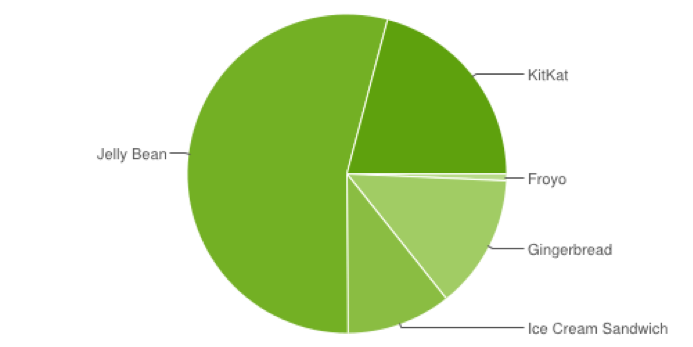
\includegraphics[width=1\textwidth]{Figuras/versionesAndroid.png}
		\rule{30em}{0.5pt}
	\caption[Gráfica de Usabilidad de las Versiones de Android]{Gráfica de Usabilidad de las Versiones de Android (Agosto 2014) \cite{devAndroid}}
	\label{fig:versionesFigura}
\end{figure}

\begin{table} 
	\begin{center}
		\begin{tabular}{|c|c|c|c|}
			\hline \rowcolor[RGB]{51,153,255} 
			\textcolor{blanco}{\bf Versión} &
				\textcolor{blanco}{\bf Nombre} &
				\textcolor{blanco}{\bf API} &
				\textcolor{blanco}{\bf Presencia en el Mercado} \\
			\hline  
				2.2 &
				Froyo &
				8 &
				0.7\% \\
      		\hline \rowcolor[RGB]{240,248,255}
      			2.3.3 - 2.3.7 &
				Gingerbread &
				10 &
				13.6\% \\
      		\hline 
      			4.0.3 - 4.0.4 &
				Ice Cream Sandwich &
				15 &
				10.6\% \\
      		\hline \rowcolor[RGB]{240,248,255}
      			4.1.x &
				Jelly Bean &
				16 &
				26.5\% \\
      		\hline 
      			4.2.x &
				Jelly Bean &
				17 &
				19.8\% \\
      		\hline \rowcolor[RGB]{240,248,255}
      			4.3 &
				Jelly Bean &
				18 &
				7.9\% \\
      		\hline 
      			4.4 &
				KitKat &
				19 &
				20.9\% \\
      		\hline 
		\end{tabular}
	\end{center}
	\caption[Usabilidad de las Versiones de Android]{Usabilidad de las Versiones de Android \cite{devAndroid}} 
	\label{tab:versionesTabla}
\end{table}

\paragraph{Lenguaje de Programación}

La fila correspondiente a lenguajes de programación en la Tabla \ref{tab:comSOM} nos muestra C, C++ y Java como los mas utilizados para Android. En la Tabla \ref{tab:paramLengu} se muestran los parámetros de los lenguajes de programación que aparecen en la Tabla \ref{tab:lenguProgra}, esto con el fin de elegir el lenguaje de programación que se utilizará en este proyecto. 

\begin{table}[h!]
	\begin{center}
		\begin{tabular}{|c|p{4.5cm}|p{4.5cm}|}
			\hline \rowcolor[RGB]{51,153,255} 
			\textcolor{blanco}{\bf Parámetro} &
				\textcolor{blanco}{\bf Descripción} &
				\textcolor{blanco}{\bf Escala de Medición} \\
			\hline 
				Paradigma &
				Enfoque empleado para modelado de un sistema según la naturaleza y filosofía de un lenguaje de programación. &
				Orientado a Objetos, Estructurado, Funcional, Reflexivo, Orientado a eventos. \\
      		\hline \rowcolor[RGB]{240,248,255}
      			Plataformas Compatibles &
				Plataforma donde el lenguaje de programación puede generar código objeto. &
				Android, iOS y Windows Phone. \\
      		\hline 
      			Curva de Aprendizaje &
				Se refiere al tiempo que lleva al equipo de desarrollo dominio y transición. &
				Corta, Media, Larga. \\
      		\hline \rowcolor[RGB]{240,248,255}
      			Complejidad &
				Es la medición relativa sobre la experiencia de trabajo con el paradigma y el lenguaje de programación que lo implementa. &
				Complejo (Sin experiencia), Media (Experiencia en paradigma o sintaxis del lenguaje), Fácil (Experiencia en paradigma y sintaxis del lenguaje). \\
      		\hline 
      			Documentación &
				Muestra la cantidad de información existente. &
				Abundante, Media, Escasa. \\
      		\hline 
    		\end{tabular}
	\end{center}
	\caption[Parámetros de Comparación para el Lenguaje de Programación]{Parámetros de Comparación para el Lenguaje de Programación} 
	\label{tab:paramLengu}
\end{table}

\begin{table} 
	\begin{center}
		\begin{tabular}{|p{3cm}|p{3cm}|p{3cm}|p{3cm}|}
			\hline \rowcolor[RGB]{51,153,255} 
			\textcolor{blanco}{\bf Parámetros} &
				\textcolor{blanco}{\bf C++} &
				\textcolor{blanco}{\bf Java} &
				\textcolor{blanco}{\bf C} \\
			\hline 
				Paradigma &
				Multiparadigma: programación orientada a objetos, programación genérica, programación estructurada, programación funcional y metaprogramación. &
				Multiparadigma: programación orientada a objetos, programación genérica, programación estructurada, programación reflexiva y programación concurrente. & 
				Programación \newline estructurada \\
      		\hline \rowcolor[RGB]{240,248,255}
      			Plataformas Compatibles &
				Multiplataforma &
				Multiplataforma &
				Multiplataforma \\
      		\hline 
      			Curva de \newline Aprendizaje &
				Media &
				Corta &
				Media \\
      		\hline \rowcolor[RGB]{240,248,255}
      			Complejidad &
				Media &
				Fácil &
				Media \\
      		\hline 
      			Documentación &
				Abundante &
				Abundante &
				Abundante \\
      		\hline 
    		\end{tabular}
	\end{center}
	\caption[Comparación de Lenguajes de Programación]{Comparación de Lenguajes de Programación} 
	\label{tab:lenguProgra}
\end{table}
\newpage
En términos de paradigma excluimos al lenguaje C ya que se requiere de programación orientada a objetos. En lo que respecta a la complejidad para el equipo de desarrollor, se muestra que Java es menos complejo que C++, por lo tanto, el lenguaje de programación que se utilizará para TASMC es Java.

\paragraph{Sistema Operativo de Escritorio}

Los sistemas operativos con los que cuenta el equipo de desarrollo se pueden observar en la Tabla \ref{tab:SOE}.

\begin{table}[h] 
	\begin{center}
		\begin{tabular}{|c|c|}
			\hline \rowcolor[RGB]{51,153,255} 
			\textcolor{blanco}{\bf Computadora} &
				\textcolor{blanco}{\bf Sistema Operativo} \\
			\hline 
				Laptop Lenovo &
				Windows 7 \\
      		\hline \rowcolor[RGB]{240,248,255}
      			MacBook Pro &
				OS X Yosemite 10.10.1 \\
      		\hline 
    		\end{tabular}
	\end{center}
	\caption[Sistemas Operativos del Equipo]{Sistemas Operativos del Equipo} 
	\label{tab:SOE}
\end{table}

Debido a que se eligió Android como sistema operativo móvil, visualizando la Tabla \ref{tab:comSOM}, encontramos que las plataformas en donde se puede desarrollar para Android son: Windows, Mac OS y Linux. Por lo tanto, las computadoras que tiene el equipo nos permiten desarrollar TASMC.

\paragraph{Entorno de Desarrollo Integrado}

Un Entorno de desarrollo integrado o IDE como se le conoce comúnmente, es una herramienta de software que permite unificar el control sobre el desarrollo de un sistema, se compone de una gran cantidad de módulos que ayudan a configurar opciones y corregir problemáticas presentes en la sintaxis o lógica del código, permiten el uso de plantillas para agilizar el desarrollo. Debido a la complejidad de los sistemas computacionales actuales, el IDE ha logrado convertirse también en una pieza clave para alcanzar la meta de desarrollo gracias a las ventajas que brinda contra los tiempos de desarrollo.

Dadas las características requeridas por las herramientas establecidas en anterioridad se priorizara que el IDE cumpla con los parámetros de la Tabla \ref{tab:paramIDEs}.

\begin{table}[h]
	\begin{center}
		\begin{tabular}{|p{4.2cm}|p{4.5cm}|p{4.5cm}|}
			\hline \rowcolor[RGB]{51,153,255} 
			\textcolor{blanco}{\bf Parámetros} &
				\textcolor{blanco}{\bf Descripción} &
				\textcolor{blanco}{\bf Escala de Medición} \\
			\hline 
				Soporte para Desarrollo Java (Android) &
				Es preciso que el IDE soporte desarrollo para el lenguaje JAVA y resguarde compatibilidad con el JDK en sus versiones 1.6 y 1.7 además de ser compatible con el ambiente de trabajo para desarrollar aplicaciones Android. &
				Con soporte, sin soporte \\
      		\hline \rowcolor[RGB]{240,248,255}
      			Soporte para Conectividad SQLite &
				Se debe tener una configuración transparente para la comunicación con SQLite, supervisada mediante el IDE. &
				Con soporte, sin soporte. \\
      		\hline 
      			Consumo de Recursos &
				El IDE debe ser congruente con el consumo de recurso, entiéndase como la exigencia de que sea una de las herramientas que consuma menos recursos para el desarrollo. &
				Alta, Media. \\
      		\hline \rowcolor[RGB]{240,248,255}
      			Eficiencia de la configuración  &
				El IDE debe realizar una configuración confiable y fácilmente modificable, para realizar pruebas antes de la puesta a punto. &
				Alta, Media, Baja. \\
      		\hline 
    		\end{tabular}
	\end{center}
	\caption[Parámetros de Comparación para IDEs]{Parámetros de Comparación para IDEs} 
	\label{tab:paramIDEs}
\end{table}

\begin{table}[h]
	\begin{center}
		\begin{tabular}{|p{3cm}|p{3cm}|p{3cm}|}
			\hline \rowcolor[RGB]{51,153,255} 
			\textcolor{blanco}{\bf Parámetros} &
				\textcolor{blanco}{\bf Android Studio} &
				\textcolor{blanco}{\bf Eclipse ADT} \\
			\hline 
				Soporte para Desarrollo Java (Android) &
				Con soporte &
				Con soporte \\
      		\hline \rowcolor[RGB]{240,248,255}
      			Soporte para Conectividad SQLite &
				Con soporte &
				Con soporte \\
      		\hline 
      			Consumo de Recursos &
				Medio &
				Alto \\
      		\hline \rowcolor[RGB]{240,248,255}
      			Eficiencia de la Configuración &
				Alta &
				Media \\
      		\hline 
    		\end{tabular}
	\end{center}
	\caption[Comparacion IDEs Android Studio y Eclipse ADT]{Comparacion IDEs Android Studio y Eclipse ADT} 
	\label{tab:comIDEs}
\end{table}

Como se puede observar Android Studio y Eclipse ADT son IDEs muy semejantes, la principal diferencia entre ambos es que Android Studio esta recibiendo más soporte que el mismo Eclipse ADT hoy en día. Debido a que Android Studio consume menos recursos y, además, el sistema de construcción que utiliza es Gradle, se utilizará éste IDE para el desarrollo de TASMC.

\paragraph{Herramienta UML}

StartUML es una de las herramientas open source para un desarrollo rápido, flexible, extensible basado en los estándares UML (Unified Modeling Lenguage) y MDA (Model Driven Arquitecture), esta herramienta corre sobre sistemas operativos Windows y Mac OS. StarUML ofrece un amplio grupo de diagramas de UML 2.0, entre los cuales están: Diagramas de casos de uso, diagrama de clases, diagrama de secuencia, diagrama de comunicación, diagrama de máquina de estado, diagrama de actividad, diagrama de componentes, diagrama de despliegue, diagrama de estructura compuesta (UML 2.0). Al igual que soporta varios lenguajes entre los cuales se encuentra Java, C++, C\# (generador de código y de ingeniería inversa). \cite{starUML}

Debido a que StarUML es gratuita, se apega a los estándares UML y se puede utilizar tanto en Windows como Mac OS, utilizaremos StarUML como herramienta UML para nuestro proyecto.
\newpage
\paragraph{Sistema Gestor de Base de Datos}

\begin{table}[h!]
	\begin{center}
		\begin{tabular}{|p{3cm}|p{5.1cm}|p{5.1cm}|}
			\hline \rowcolor[RGB]{51,153,255} 
			\textcolor{blanco}{\bf Parámetro} &
				\textcolor{blanco}{\bf SQLite} &
				\textcolor{blanco}{\bf Oracle Lite} \\
			\hline 
				Paradigma &
				Relacional &
				Relacional \\
      		\hline \rowcolor[RGB]{240,248,255}
      			Costo de Licencia &
				SQLite es de dominio público, y por tanto, no tiene costo y se puede redistribuir libremente. &
				\$ 180 USD por licencia \\
      		\hline 
      			Interfaces &
				Cuenta con diferentes interfaces del API para trabajar con C++, PHP, Perl, Python, etc. &
				Interfaz GUI y SQL. \\
      		\hline \rowcolor[RGB]{240,248,255}
      			Tamaño &
				SQLite tiene una pequeña memoria y una única biblioteca es necesaria para acceder a bases de datos, esto lo hace ideal para aplicaciones de bases de datos incorporadas. El tamaño máximo de una base de datos es de 2 TB. &
				 La carga sobre el dispositivo móvil es mínima ya que los datos y aplicaciones se almacenan en servidores móviles los cuales a su vez se comunican con un repositorio propio de Oracle. \\
      		\hline 
      		Portabilidad &
      		Se ejecuta en muchas plataformas y sus bases de datos pueden ser fácilmente portadas sin ninguna configuración o administración. &
      		Se ejecuta en múltiples plataformas, incluyendo Android, iPhone (Apple iOS), Blackberry, Symbian OS, Windows de 32 bits, Windows Mobile, Linux y otras plataformas de dispositivos móviles. \\
      		\hline \rowcolor[RGB]{240,248,255}
      		Rendimiento &
      		SQLite realiza operaciones de manera eficiente y es más rápido que MySQL y PostgreSQL. &
      		Ofrece un rendimiento fuera de la caja, permitiendo a los usuarios el acceso información de forma rápida y eficiente. Multiprocesador y la memoria caché dinámica dimensionamiento garantizar arriba rendimiento para las bases de datos más grandes y un mayor número de usuarios conectados. \\ 
      		\hline 
      		Estabilidad &
      		SQLite es compatible con ACID, reunión de los cuatro criterios de Atomicidad, Consistencia, Aislamiento y Durabilidad. &
      		Oracle es compatible con ACID, además de manejar integridad referencial, transacciones y  estándar de codificación Unicode. \\
      		\hline
    		\end{tabular}
	\end{center}
	\caption[Comparación SGBD móviles]{Comparación SGBD móviles} 
	\label{tab:comSGBD}
\end{table}
\newpage
El gestor de base de datos es el software que se ocupa del almacenamiento, modificación y extracción de la información procedente de una base de datos. Representa una interfaz de comunicación entre la entrada de información y los registros almacenados en repositorios. Además forma parte medular para la implementación de todo sistema que almacena información en bases de datos. En la Tabla \ref{tab:comSGBD} se encuentran los SGBD, para móviles, que se pueden utilizar para el desarrollo de TASMC.

En términos de consumo de recursos, rendimiento y costo se eligió utilizar SQLite como gestor de base de datos, dado que para la implementación del sistema se pensó en utilizar un SGBD capaz de reaccionar ágilmente ante la concurrencia de solicitudes al tiempo que consume bajos recursos, además de que no es necesario una base de datos tan robusta.

\paragraph{API de Rutas de Google Maps}

El API de rutas de Google es un servicio que utiliza una solicitud HTTP para calcular rutas para llegar de una ubicación a otra. Puedes buscar rutas de varios métodos de transporte, como en transporte público, en coche, a pie o en bicicleta. Las rutas pueden especificar los orígenes, los destinos y los hitos como cadenas de texto (por ejemplo, ``Chicago, IL'' o ``Darwin, NT, Australia'') o como coordenadas de latitud/longitud. El API de rutas puede devolver rutas segmentadas mediante una serie de hitos.

Por lo general, este servicio está diseñado para calcular rutas a partir de direcciones estáticas (conocidas previamente) para la ubicación del contenido de la aplicación en un mapa. Sin embargo, este servicio no está diseñado para responder en tiempo real a la información introducida por el usuario.

El cálculo de indicaciones es un proceso que consume mucho tiempo y muchos recursos. Siempre que sea posible, se debe realiza un cálculo previo de las direcciones conocidas (mediante el servicio descrito) y almacena los resultados en una memoria caché. \cite{apiGoogleMaps}
\newpage
\paragraph{API de IndoorAtlas}

El API de Indooratlas nos ayudará a realizar la localización en interiores sin necesidad de utilizar infraestructura de hardware externo. \cite{apiIndoorAtlas}

Lo que Indooratlas nos ofrece:

\begin{itemize}
	\item 2 metros de precisión en la localización.
	\item	Ahorro de recursos si lo comparamos con otra técnica para la localización en interiores.
	\item Una solución multiplataforma para iOS y Android.
\end{itemize}

\subsection{Factibilidad Ecónomica}

El estudio de factibilidad económica permite analizar los costos y beneficios económicos que se obtendrán con el desarrollo del proyecto, sin importar que la implementación de nuestro sistema sea un prototipo sin fines lucrativos. 
\vspace{2cm}
\begin{table}[h]
	\begin{center}
		\begin{tabular}{|c|c|c|c|c|}
			\hline \rowcolor[RGB]{51,153,255} 
			\textcolor{blanco}{\bf Recurso} &
				\textcolor{blanco}{\bf Cantidad} &
				\textcolor{blanco}{\bf Meses} &
				\textcolor{blanco}{\bf Salario Mensual} &
				\textcolor{blanco}{\bf Total} \\
			\hline 
				Líder de proyecto &
				1 &
				8 &
				\$ 35,000.00 &
				\$ 280,000.00 \\
      		\hline \rowcolor[RGB]{240,248,255}
      			Desarrollador &
				2 &
				8 &
				\$ 23,000.00 &
				\$ 368,000.00 \\
      		\hline 
    		\end{tabular}
	\end{center}
	\caption[Recursos Humanos]{Recursos Humanos \cite{salarios}} 
	\label{tab:recursosHumanos}
\end{table}

\begin{table}[h]
	\begin{center}
		\begin{tabular}{|c|c|c|c|}
			\hline \rowcolor[RGB]{51,153,255} 
			\textcolor{blanco}{\bf Recurso} &
				\textcolor{blanco}{\bf Cantidad} &
				\textcolor{blanco}{\bf Precio Unitario} &
				\textcolor{blanco}{\bf Total} \\
			\hline
				Impresiones y fotocopias &
				5,000 &
				\$ 0.50 &
				\$ 2,500.00  \\
      		\hline \rowcolor[RGB]{240,248,255}
      			Gastos varios &
				&
				&
				\$ 500.00 \\
      		\hline 
    		\end{tabular}
	\end{center}
	\caption[Recursos Consumibles]{Recursos Consumibles} 
	\label{tab:recursosConsumibles}
\end{table}

\begin{table}[h] 
	\begin{center}
		\begin{tabular}{|c|c|c|c|}
			\hline \rowcolor[RGB]{51,153,255} 
			\textcolor{blanco}{\bf Recurso} &
				\textcolor{blanco}{\bf Cantidad} &
				\textcolor{blanco}{\bf Costo} &
				\textcolor{blanco}{\bf Total} \\
			\hline 
				Laptop Lenovo &
				1 &
				\$ 9,000.00 &
				\$ 9,000.00  \\
      		\hline \rowcolor[RGB]{240,248,255}
      			MacBook Pro &
				1 &
				\$ 19,000.00&
				\$ 19,000.00 \\
			\hline 
				Samsung Galaxy S4 &
				1 &
				\$ 7,000.00 &
				\$ 7,000.00  \\
      		\hline \rowcolor[RGB]{240,248,255}
      			Google Maps Services &
				1 &
				\$ 0 &
				\$ 0 \\
			\hline
				IndoorAtlas Services &
				1 &
				\$ 0 &
				\$ 0 \\
      		\hline \rowcolor[RGB]{240,248,255}
      			Web Service Vuelos &
				1 &
				\$ 0 &
				\$ 0 \\
			\hline
				Servidor TASMC &
				1 &
				\$ 4,000.00 &
				\$ 4,000.00 \\	
      		\hline 
    		\end{tabular}
	\end{center}
	\caption[Recursos Tecnológicos]{Recursos Tecnológicos} 
	\label{tab:recursosTecnologicos}
\end{table}

\begin{table} 
	\begin{center}
		\begin{tabular}{|c|c|}
			\hline \rowcolor[RGB]{51,153,255} 
			\textcolor{blanco}{\bf Recurso} &
				\textcolor{blanco}{\bf Total} \\
			\hline 
				Recursos Humano &
				\$ 648,000.00  \\
      		\hline \rowcolor[RGB]{240,248,255}
      			Recursos Consumibles &
				\$ 3,000.00  \\
			\hline 
				Recursos Tecnológicos &
				\$ 39,000.00  \\
      		\hline \rowcolor[RGB]{240,248,255}
      			Subtotal &
				\$ 690,000.00  \\
			\hline  
				Imprevistos (10 \%) &
				\$ 70,000.00  \\
      		\hline \rowcolor[RGB]{240,248,255}
      			Total &
				\$ 760,000.00 \\
      		\hline 
    		\end{tabular}
	\end{center}
	\caption[Costo Total TASMC]{Costo Total TASMC} 
	\label{tab:costoTasmc}
\end{table}
\vspace{3cm}
\newpage
\subsection{Factibilidad Operativa}

El estudio de factibilidad operativa nos ayuda a determinar si el proyecto puede ser implementado y completado para lograr sus objetivos. Puede ser visto desde dos puntos: recursos humanos para la implementación del proyecto y recursos necesarios para la puesta en marcha del proyecto. 

\textbf{Recursos humanos para la implementación del proyecto}

El equipo de trabajo cuenta con los conocimientos necesarios para el desarrollo del proyecto, mediante las tecnologías seleccionadas. Por lo que es factible que el proyecto sea implementado. 

\textbf{Recursos necesarios para la puesta en marcha del proyecto}

El proyecto se quedará como un prototipo, por lo que no se necesitan recursos extras para una implantación y puesta en marcha del sistema dentro de una empresa, aunque el proyecto puede ser extendido o mejorado para su implantación.

En la Tabla \ref{tab:fodaTASMC} se muestra el FODA de TASMC:

\begin{table}[h]
	\begin{center}
		\begin{tabular}{|p{6.8cm}|p{6.8cm}|}
			\hline  
				\textbf{\small Fortalezas:} & \textbf{\small Debilidades:} \\
				{\parbox{0.45\textwidth}{
					\begin{itemize}
                			\item \small Ser un sistema único de gestión integral de viajes.
						\item \small Creación de un sistema totalmente personalizado y a la medida.
						\item \small Preocupación y esmero por el buen diseño estético y  funcional de la aplicación.
           			\end{itemize} }} &
				{\parbox{0.45\textwidth}{
					\begin{itemize}
                			\item \small Poca publicidad de la aplicación.
						\item \small No contar con los planos del AICM.
						\item \small Menor disponibilidad de recursos. 
           			\end{itemize} }}	\\
			\hline 
			\textbf{\small Oportunidades:} & \textbf{\small Amenazas:} \\
				{\parbox{0.45\textwidth}{
					\begin{itemize}
                			\item \small Ampliación de mercado en el desarrollo de aplicaciones móviles.
						\item \small Alta intensidad en el uso de aplicaciones móviles.
           			\end{itemize} }} &
				{\parbox{0.45\textwidth}{
					\begin{itemize}
                			\item \small Compañías transnacionales que se dedican al desarrollo de aplicaciones móviles. 
						\item \small Posible existencia de aplicaciones similares que cuenten con mejor infraestructura de operación. 
           			\end{itemize} }}	\\
			\hline 
		\end{tabular}
	\end{center}
	\caption[FODA TASMC]{FODA TASMC} 
	\label{tab:fodaTASMC}
\end{table}
\section{Análisis de Requerimientos}

Dentro de esta etapa, a partir de las reglas de negocio y la descripción del sistema se debe considerar la obtención de los requerimientos básicos, los cuales cumplen la función de definir de manera general el sistema a desarrollar para después pasar a especificar los requerimientos funcionales que nos reflejen a detalle las funciones que el sistema debe o no efectuar.

Los requerimientos no funcionales son restricciones a las funciones del sistema o bien cualidades que este debe de presentar para considerarle un sistema de calidad.

\subsection{Reglas de Negocio}

Las reglas de negocio especifican procesos, operaciones, normas y restricciones consideradas en el desarrollo de software dependiendo de la metodología que se emplea para resolver el problema y lograr los objetivos. Las reglas del negocio son usadas para verificar que ciertos comportamientos se cumplan y en caso de que se presente una excepción conocer las alternativas para la solución del problema.

\begin{table}
	\begin{center}
		\begin{tabular}{|c|c|p{3cm}|p{5.7cm}|}
			\hline \rowcolor[RGB]{0,102,204} 
				\textcolor{blanco}{\bf Identificador} &
				\textcolor{blanco}{\bf Tipo} &
				\textcolor{blanco}{\bf Nombre} &
				\textcolor{blanco}{\bf Descripción} \\
			\hline \rowcolor[RGB]{224,224,224} 
				\textbf{RN01} &
				Definición &
				Viajero aéreo &
				Persona que viaja en un avión. \\
      		\hline 
      			\textbf{RN02} &
				Definición &
				Viaje aéreo &
				Traslado de un lugar a otro, mediante la  utilizando aeronaves, con fin lucrativo. \\
			\hline \rowcolor[RGB]{224,224,224} 
				\textbf{RN03} &
				Definición &
				Aerolínea &
				Empresa o compañía dedicada al transporte aéreo. \\ 
			\hline
				\textbf{RN04} &
				Definición &
				Vuelo &
				Trayecto que realiza un avión, haciendo o no escalas, entre el punto de origen y el destino. \\ 
			\hline \rowcolor[RGB]{224,224,224} 
				\textbf{RN05} &
				Hecho &
				Visualizar los vuelos de las aerolíneas. &
				El viajero aéreo puede ver todos los vuelos que las aerolíneas proporcionan, sin importar que falten semanas o meses para el vuelo. \\ 
			\hline
				\textbf{RN06} &
				Definición &
				Itinerario de viaje &
				Listado en el que se describen los lugares por los que se va a pasar. \\ 
			\hline \rowcolor[RGB]{224,224,224} 
				\textbf{RN07} &
				Hecho &
				Notificar al viajero &
				El viajero debe ser notificado en caso de producirse algún cambio en cuanto al vuelo o el horario. \\ 
			\hline
				\textbf{RN08} &
				Hecho &
				Recordar documentos importantes &
				Se debe apoyar al viajero en que no olvide documentos importantes para su viaje. \\ 
			\hline \rowcolor[RGB]{224,224,224} 
				\textbf{RN09} &
				Hecho &
				Puntualidad en el aeropuerto &
				El viajero debe llegar puntual a la cita en el aeropuerto para cumplir con los procedimientos que necesita para el abordaje del avión. \\ 
			\hline
				\textbf{RN10} &
				Hecho &
				Guardar objetos importantes &
				El viajero no debe olvidar objetos importantes para contribuir con la satisfacción total del viaje. \\ 
			\hline \rowcolor[RGB]{224,224,224} 
				\textbf{RN11} &
				Hecho &
				Hoteles en la ciudad destino &
				Se debe informar al viajero sobre los hoteles que se encuentren en la ciudad destino.  \\ 
			\hline
				\textbf{RN12} &
				Hecho &
				Usabilidad &
				Se debe asistir al viajero, para que pueda cumplir con un viaje satisfactorio, apoyándolo con la gestión de su viaje de una manera sencilla y comprensible.  \\ 
			\hline \rowcolor[RGB]{224,224,224} 
				\textbf{RN13} &
				Hecho &
				Disponibilidad &
				La información debe estar disponible idealmente todo el año.  \\ 
			\hline
				\textbf{RN14} &
				Hecho &
				Información del AICM &
				El viajero debe conocer el teléfono, dirección, mapa, etc. del aeropuerto para cualquier situación o necesidad que se presente. \\ 
			\hline 
		\end{tabular}
	\end{center}
	\caption[Reglas de Negocio]{Reglas de Negocio} 
	\label{tab:reglasNegocio}
\end{table}

\subsection{Requerimientos Básicos (RB)}

Las características que contendrá TASMC son las siguientes:

\begin{itemize}
	\item Guardar configuración personal de cada usuario al registrarse
	\item Búsqueda de Hoteles
	\item Lista de Hoteles
	\item Búsqueda de Vuelos
	\item Lista de Vuelos
	\item Lista de información del AICM
	\item Lista de Objetos para viaje
	\item Itinerario de viaje
	\item Ruta casa-aeropuerto
	\item Ubicación dentro del Aeropuerto
\end{itemize}

En base a las características que debe contener TASMC se han podido identificar los diferentes módulos de la aplicación que se encuentran listados a continuación:

\textbf{Módulo de Registro/Configuración}

\begin{itemize}
	\item Correo electrónico.
	\item Clase de vuelo preferida.
	\item Cantidad preferida de estrellas en hotel. 
\end{itemize}

\textbf{Módulo de Hoteles}

\begin{itemize}
	\item Búsqueda de Hoteles.
	\begin{itemize}
		\item Número de Huéspedes.
		\item Número de Habitaciones.
		\item Fecha de entrada y salida.
	\end{itemize}
	\item Listado de Hoteles.
	\item Detalle de Hoteles.
	\item Filtros según:
	\begin{itemize}
		\item Estrellas: de 1 a 5.
		\item Estrellas: de 5 a 1.
		\item Precios de bajo a alto.
		\item Precios de alto a bajo.
	\end{itemize}
\end{itemize}

\textbf{Modulo de Vuelos}
 
\begin{itemize}
	\item Búsqueda de Vuelos
	\begin{itemize}
		 \item Número de pasajeros.
		\item Clase (Económico, Económico Premium, Business, Primera, Todas).
		\item Fechas (Salida y llegada).
		\item Ciudad origen – Ciudad destino.
	\end{itemize}
	\item Listado de Vuelos.
	\item Detalle de Vuelos.
	\item Filtros según:
	\begin{itemize}
		\item Precios de bajo a alto.
		\item Precios de alto a bajo.
		\item Clase de vuelo.
	\end{itemize}
\end{itemize}

\textbf{Información Aeropuerto AICM}

\begin{itemize}
	\item Información de Aeropuerto AICM
	\begin{itemize}
		 \item Sitio web AICM.
		\item Teléfono AICM.
		\item Ubicación.
	\end{itemize}
	\item Mapa del Aeropuerto.
	\item	Servicios en el Aeropuerto.
\end{itemize}

\textbf{Lista de equipaje}

\begin{itemize}
	\item 	Lista de equipaje por tipo de vuelo.
	\item Lista de equipaje.
	\item Añadir nueva lista.
	\item Añadir nuevo objeto.
	\item Documentos importantes
\end{itemize}
	
\textbf{Itinerario}

\begin{itemize}
	\item Alarma según tipo de vuelo:
	\begin{itemize}
		\item Nacional 3.5 Horas antes de hora de salida.
		\item Internacional 4.5 Horas antes de hora de salida.
	\end{itemize}
	\item Información de vuelo
	\begin{itemize}
		\item Número de vuelo.
		\item Hora de salida.
		\item Hora de llegada.
	\end{itemize}
	\item Itinerario de viaje
	\begin{itemize}
	 \item Actividades a realizar durante el viaje.
	\end{itemize}
\end{itemize}

\textbf{Ruta para llegar al AICM}

\begin{itemize}
	\item Visualizar una ruta para llegar al AICM.
\end{itemize}

\textbf{Ubícate}

\begin{itemize}
	\item Ubicar sala de abordaje del usuario.
	\item Ubicar servicios del AICM.
\end{itemize} 

\textbf{Información de Vuelo}

\begin{itemize}
	\item Número de vuelo.
	\item Estado de vuelo.
	\item Ciudad de origen.
	\item Ciudad destino.
	\item Hora de salida.
	\item Hora de llegada.
	\item Fecha.
	\item Terminal.
	\item Puerta.
\end{itemize}

\begin{table}
	\begin{center}
		\begin{tabular}{|c|p{8.4cm}|p{2.5cm}|}
			\hline \rowcolor[RGB]{0,102,204} 
				\textcolor{blanco}{\bf Identificador} &
				\textcolor{blanco}{\bf Descripción} &
				\textcolor{blanco}{\bf Origen} \\
			\hline \rowcolor[RGB]{224,224,224} 
				\textbf{RB01} &
				Módulo que permita al usuario realizar su registro a TASMC y elegir sus preferencias. &
				Definición del sistema  \\
      		\hline 
      			\textbf{RB02} &
				Módulo para realizar búsquedas de Hoteles y posteriormente generar un listado de dicha búsqueda. &
				Definición del sistema, RN11 \\
			\hline \rowcolor[RGB]{224,224,224} 
				\textbf{RB03} &
				Módulo para realizar búsquedas de Vuelos y posteriormente generar un listado de dicha búsqueda. &
				Definición del sistema, RN05 \\ 
			\hline
				\textbf{RB04} &
				Módulo para visualizar la información del AICM, como sitio web, teléfono, ubicación y redes sociales. &
				Definición del sistema, RN14 \\ 
			\hline \rowcolor[RGB]{224,224,224} 
				\textbf{RB05} &
				Módulo para la gestión de objetos, donde el usuario podrá verificar en una lista los objetos requeridos para su viaje. &
				Definición del sistema, RN10 \\ 
			\hline
				\textbf{RB06} &
				Módulo para asistir en la construcción del itinerario de viaje del usuario. &
				Definición del sistema \\ 
			\hline \rowcolor[RGB]{224,224,224} 
				\textbf{RB07} &
				Módulo que permita visualizar rutas que tengan como destino el AICM. &
				Definición del sistema, RN09, RN12 \\ 
			\hline
				\textbf{RB08} &
				Módulo que permita visualizar en un mapa del AICM la ubicación del usuario en el momento que lo requiera. &
				Definición del sistema, RN12 \\ 
			\hline \rowcolor[RGB]{224,224,224} 
				\textbf{RB09} &
				Módulo para visualizar la información del vuelo, como lo es, el número de vuelo, el estado de vuelo, ciudad de origen, ciudad destino, hora de salida, hora de llegada, fecha, terminal y puerta. &
				Definición del sistema, RN07 \\ 
			\hline 
		\end{tabular}
	\end{center}
	\caption[Requerimientos Básicos]{Requerimientos Básicos} 
	\label{tab:reqBasicos}
\end{table}

\subsection{Requerimientos Funcionales (RF)}

En la siguiente tabla se muestran los requerimientos funcionales de TASMC:

\begin{table}
	\begin{center}
		\begin{tabular}{|c|p{9.4cm}|p{1.5cm}|}
			\hline \rowcolor[RGB]{0,102,204} 
				\textcolor{blanco}{\bf Identificador} &
				\textcolor{blanco}{\bf Descripción} &
				\textcolor{blanco}{\bf Origen} \\
			\hline \rowcolor[RGB]{224,224,224} 
				\textbf{RF01} &
				El sistema debe ser capaz de configurar gustos y posibilidades económicas del viajero para generar un mejor resultado en la búsqueda de vuelos y hoteles. &
				RB01 \\
      		\hline 
      			\textbf{RF02} &
				El usuario debe poder visualizar sugerencias de hoteles disponibles,  según una búsqueda que haya realizado previamente. &
				RB02 \\
			\hline \rowcolor[RGB]{224,224,224} 
				\textbf{RF03} &
				El usuario debe poder visualizar sugerencias de vuelos disponibles, según una búsqueda que haya realizado previamente. &
				RB03 \\ 
			\hline
				\textbf{RF04} &
				El sistema debe ser capaz de generar una lista de objetos que debe empacar el usuario, según el tipo de viaje que se seleccione. &
				RB05 \\ 
			\hline \rowcolor[RGB]{224,224,224} 
				\textbf{RF05} &
				El sistema debe proporcionar una lista que permita al usuario generar un itinerario de viaje. &
				RB06 \\ 
			\hline
				\textbf{RF06} &
				El sistema mostrará una sugerencia de la mejor ruta para llegar al AICM desde la posición actual del usuario. &
				RB07 \\ 
			\hline \rowcolor[RGB]{224,224,224} 
				\textbf{RF07} &
				El sistema debe ser capaz de ubicar al usuario dentro del AICM y facilitarle la llegada a su sala de abordaje. &
				RB08 \\ 
			\hline
				\textbf{RF08} &
				El sistema deberá mostrar la información del número de vuelo, estado de vuelo, ciudades de origen y destino, 					hora de salida y llegada, fecha, terminal y puerta. &
				RB09 \\ 
			\hline
		\end{tabular}
	\end{center}
	\caption[Requerimientos Funcionales]{Requerimientos Funcionales} 
	\label{tab:reqFuncionales}
\end{table}

\subsection{Requerimientos No Funcionales (RNF)}

En la siguiente tabla se muestran los requerimientos no funcionales de TASMC:

\begin{table}
	\begin{center}
		\begin{tabular}{|c|p{8.4cm}|p{2.5cm}|}
			\hline \rowcolor[RGB]{0,102,204} 
				\textcolor{blanco}{\bf Identificador} &
				\textcolor{blanco}{\bf Descripción} &
				\textcolor{blanco}{\bf Origen} \\
			\hline \rowcolor[RGB]{224,224,224} 
				\textbf{RNF01} &
				Las condiciones del entorno no deben de afectar la localización del usuario. Se debe de considerar un ambiente controlado. &
				RB08 \\
      		\hline 
      			\textbf{RNF02} &
				La aplicación debe funcionar en todos los dispositivos móviles que contengan el sistema operativo Android versión 4.4 (KitKat). &
				Definición del Sistema \\
			\hline \rowcolor[RGB]{224,224,224} 
				\textbf{RNF03} &
				Se debe de presentar una interfaz gráfica para poder seleccionar las distintas funciones que puede utilizar el usuario en el sistema. &
				RN12 \\ 
			\hline
				\textbf{RNF04} &
				El sistema debe enviar una respuesta con una rapidez acorde al ancho de banda y la disponibilidad de la red. &
				Definición del Sistema \\ 
			\hline \rowcolor[RGB]{224,224,224} 
				\textbf{RNF05} &
				El sistema debe tener la posibilidad de generar ampliaciones de funcionalidad y escalabilidad. &
				Definición del Sistema \\ 
			\hline
				\textbf{RNF06} &
				Se debe dar soporte continuo al sistema. &
				RN12 \\ 
			\hline \rowcolor[RGB]{224,224,224} 
				\textbf{RNF07} &
				La navegación del usuario dentro de la aplicación debe ser de fácil entendimiento y de manera intuitiva. &
				RB12 \\ 
			\hline
		\end{tabular}
	\end{center}
	\caption[Requerimientos No Funcionales]{Requerimientos No Funcionales} 
	\label{tab:reqNoFuncionales}
\end{table}
\section{Análisis de Riesgos}

El proceso de análisis de riesgos es de utilidad para conocer y de alguna manera tratar de reducir algunas actividades, ideas o actitudes que amenazan con la completa y eficaz elaboración del proyecto.

El primer paso para llevar a cabo el análisis de riesgos es identificarlos. Una manera sencilla para identificar los riesgos es incluirlos dentro de alguna de las siguientes clasificaciones: riesgos organizacionales, riesgos sobre el personal, riesgos tecnológicos, riesgos sobre cambios en los requerimientos y riesgos sobre las herramientas.

Una vez identificados y clasificados los riesgos se hace una valoración de la probabilidad de ocurrencia que tiene cada uno mediante una clasificación por rangos de probabilidad como la Tabla \ref{tab:probabilidadRiesgos}.

\begin{table}[h]
	\begin{center}
		\begin{tabular}{|c|c|}
			\hline \rowcolor[RGB]{51,153,255} 
				\textcolor{blanco}{\bf Probabilidad en \%} &
				\textcolor{blanco}{\bf Valoración} \\
			\hline 
				0\% - 10\% &
				Muy bajo \\
      		\hline \rowcolor[RGB]{240,248,255}
				10\% - 25\% &
				Bajo \\
			\hline 
				25\% - 50\% &
				Moderado \\ 
			\hline \rowcolor[RGB]{240,248,255}
				50\% - 75\% &
				Alto \\ 
			\hline
				75\% - 100\% &
				Muy Alto \\ 
			\hline
		\end{tabular}
	\end{center}
	\caption[Clasificación de Riesgos Conforme a su Probabilidad]{Clasificación de Riesgos Conforme a su Probabilidad} 
	\label{tab:probabilidadRiesgos}
\end{table}

Una vez que cada riesgo tiene asignada una valoración se procede a determinar el efecto que el riesgo tendrá en caso de que se llegara a cumplir. Una manera sencilla para determinar el efecto de cada riesgo es asignar una de las siguientes clasificaciones: catastrófico, serio, tolerable e insignificante. Cada una de las clasificaciones anteriores está ordenada en forma descendente conforme a la valoración de su impacto.

Cuando se han seguido todos los pasos para el proceso de análisis de riesgos el resultado es una tabla donde se muestra el nombre del riesgo, su clasificación, su valoración y su impacto. Los riesgos presentados en la Tabla \ref{tab:analisisRiesgos} deben ser ordenados de manera descendente conforme a su impacto.

\begin{table}[h]
	\begin{center}
		\begin{tabular}{|>{\columncolor[RGB]{51,153,255}}p{6.6cm}|c|c|c|}
			\hline \rowcolor[RGB]{51,153,255} 
				\textcolor{blanco}{\bf Riesgo} &
				\textcolor{blanco}{\bf Clasificación} &
				\textcolor{blanco}{\bf Valoración} &
				\textcolor{blanco}{\bf Efecto} \\		
			\hline
				\textcolor{blanco}{\bf Mala comunicación entre los integrantes del equipo} &
				Organizacional &
				Alto &
				Serio \\
			\hline
				\textcolor{blanco}{\bf Recursos insuficientes para concluir el proyecto} &
				\cellcolor[RGB]{240,248,255}  Organizacional &
				\cellcolor[RGB]{240,248,255}Alto &
				\cellcolor[RGB]{240,248,255}Serio \\
      		\hline 
				\textcolor{blanco}{\bf Retraso de las actividades del proyecto} &
				Organizacional &
				Bajo &
				Serio \\
			\hline  
				\textcolor{blanco}{\bf Falta de responsabilidad de los integrantes del equipo} &
				\cellcolor[RGB]{240,248,255}Personal &
				\cellcolor[RGB]{240,248,255}Bajo &
				\cellcolor[RGB]{240,248,255}Serio \\
			\hline
				\textcolor{blanco}{\bf Mala distribución de actividades} &
				Organizacional &
				Bajo &
				Serio \\
			\hline 
				\textcolor{blanco}{\bf Permiso denegado para realizar trabajos dentro del AICM} &
				\cellcolor[RGB]{240,248,255}Tecnológico &
				\cellcolor[RGB]{240,248,255}Moderado &
				\cellcolor[RGB]{240,248,255}Serio \\
			\hline
				\textcolor{blanco}{\bf Mal control de las versiones del proyecto.} &
				Organizacional &
				Moderado &
				Serio \\
			\hline 
				\textcolor{blanco}{\bf Baja definitiva de alguno de los integrantes del equipo.} &
				\cellcolor[RGB]{240,248,255}Personal &
				\cellcolor[RGB]{240,248,255}Muy Bajo &
				\cellcolor[RGB]{240,248,255}Serio \\
			\hline
				\textcolor{blanco}{\bf Cambios en los requerimientos del sistema por parte de los sinodales} &
				Requerimientos &
				Alto &
				Serio \\
			\hline 
				\textcolor{blanco}{\bf Enfermedad de alguno de los miembros del equipo.} &
				\cellcolor[RGB]{240,248,255}Personal &
				\cellcolor[RGB]{240,248,255}Bajo &
				\cellcolor[RGB]{240,248,255}Tolerable \\
			\hline
				\textcolor{blanco}{\bf Rendimiento no competitivo del sistema} &
				Tecnológico &
				Alto &
				Serio \\
			\hline 
				\textcolor{blanco}{\bf Ausencia de algún integrante del equipo por un periodo prolongado de tiempo} &
				\cellcolor[RGB]{240,248,255}Personal &
				\cellcolor[RGB]{240,248,255}Muy Alto &
				\cellcolor[RGB]{240,248,255}Tolerable \\
			\hline
				\textcolor{blanco}{\bf Falta de dominio de las herramientas de desarrollo} &
				Personal &
				Moderado &
				Tolerable \\
			\hline 
				\textcolor{blanco}{\bf Falla en los dispositivos móviles de prueba} &
				\cellcolor[RGB]{240,248,255}Tecnológico &
				\cellcolor[RGB]{240,248,255}Alto &
				\cellcolor[RGB]{240,248,255}Tolerable \\
			\hline
				\textcolor{blanco}{\bf Funcionamiento inadecuado en la implementación de alguna tecnología después de haber sido calificada como adecuada en el Estudio de Factibilidad} &
				Tecnológico &
				Alto &
				Serio \\
			\hline 
				\textcolor{blanco}{\bf Incorrecta definición de la problemática del proyecto} &
				\cellcolor[RGB]{240,248,255}Organizacional &
				\cellcolor[RGB]{240,248,255}Muy Alto &
				\cellcolor[RGB]{240,248,255}Serio \\
			\hline
		\end{tabular}
	\end{center}
	\caption[Análisis de Riesgos]{Análisis de Riesgos} 
	\label{tab:analisisRiesgos}
\end{table}

\textbf{Identificación de Riesgos}
\newline
Los riesgos han sido identificados clasificados, según el foco de interés, de la siguiente manera:

\begin{itemize}
	\item Ambiente del proyecto
	\item Inventario de activos e intangibles
	\item Mantenimiento de software y hardware
	\item Equipo de trabajo 
	\item Errores de estimación de costos 
\end{itemize}
\clearpage
\textbf{Estrategias para la mitigación de riesgos}
\newline

\begin{table}[h]
	\begin{center}
		\begin{tabular}{|p{14.2cm}|}
			\hline \rowcolor[RGB]{51,153,255} 
				\textcolor{blanco}{\bf Estrategia de mitigación} \\ 
			\hline 
				Seguimiento semanal de los hitos definidos por cada actividad en el desarrollo del proyecto. \\
      		\hline \rowcolor[RGB]{240,248,255} 
				Continúa capacitación del personal durante las horas de trabajo. \\
			\hline 
				Designación de considerable tiempo para esta actividad. \\ 
			\hline \rowcolor[RGB]{240,248,255}
				Conocimiento y seguimiento de la situación laboral y personal de cada miembro del equipo. \\ 
			\hline 
				Realización de pruebas como actividades de capacitación de las tecnologías a usar antes de ser implementadas. \\ 
			\hline \rowcolor[RGB]{240,248,255}
				Realización de pruebas al sistema para poder evitar el mal funcionamiento de alguno de los módulos \\ 
			\hline
				Planificación de todas las actividades antes de comenzar con el proyecto y fijar una fecha de entrega anterior a la acordada con el cliente pues esto nos dará una holgura de tiempo \\ 
			\hline \rowcolor[RGB]{240,248,255}
				Buscar y utilizar herramientas que se adapten a todos los dispositivos \\ 
			\hline
				Mantener una actitud positiva para manejar  los problemas y regirse conforme a la planeación \\ 
			\hline
		\end{tabular}
	\end{center}
	\caption[Plan de Mitigación]{Plan de Mitigación} 
	\label{tab:planMitigacion}
\end{table}

\textbf{Planes de contingencia}
\newline

\begin{table}[h]
	\begin{center}
		\begin{tabular}{|p{14.2cm}|}
			\hline \rowcolor[RGB]{51,153,255} 
				\textcolor{blanco}{\bf Planes de contingencia} \\
			\hline 
				Compensar el tiempo de retraso con horas de trabajo extra. \\
      		\hline \rowcolor[RGB]{240,248,255}
				Capacitación personal para el personal incompetente en horas extra de trabajo. \\
			\hline 
				Dialogo en el  equipo de trabajo si existe una mala definición en la problemática del proyecto para hacer un replanteamiento de la problemática. \\ 
			\hline \rowcolor[RGB]{240,248,255}
				Distribución del trabajo entre los miembros del equipo aumentando jornadas de trabajo. \\ 
			\hline 
				Elección de una tecnología secundaria compatible con el proyecto. \\ 
			\hline \rowcolor[RGB]{240,248,255}
				Ocupar la holgura de tiempo y trabajar más del tiempo estipulado. \\ 
			\hline
				Reparar el modulo o crear uno nuevo para evitar contratiempos. \\ 
			\hline
		\end{tabular}
	\end{center}
	\caption[Plan de Contingencia]{Plan de Contingencia} 
	\label{tab:planContingencia}
\end{table}

\begin{center}
	{\bf \underline{\small Observación: Todos los riesgos antes mencionados pueden presentarse en cualquier parte}}
	{\bf \underline{\small del proyecto por eso  los planes de mitigación y/o contingencia no han sido fechados.}}
\end{center} 
% Capitulo 6

\chapter{Configuración del Ambiente de Desarrollo} % Main chapter title

\label{ConfiguracionAmbienteDesarrollo} % For referencing the chapter elsewhere, use \ref{Chapter1} 

\lhead{Capítulo 6 \emph{Configuración del Ambiente de Desarrollo}} % This is for the header on each page - perhaps a shortened title

Esta tarea consiste en configurar los ambientes tanto físicos como técnicos para el proyecto. Esta tarea involucra a los desarrolladores de software en el ambiente técnico de desarrollo, además se realizan pruebas de concepto sin necesariamente implementar un requerimiento.

\section{Configuración Web Service}

\begin{itemize}
	\item \textbf{Nombre aplicación: } TASMC.
	\item \textbf{Tipo de Proyecto: } PHP Application.
	\item \textbf{Framework: } nusoap.php
\end{itemize}

\section{Configuración Aplicación Móvil }

\begin{itemize}
	\item \textbf{Nombre aplicación: } TASMC.
	\item \textbf{Tipo de Proyecto: } Blank Activity.
	\item \textbf{SDK Mínimo Requerido: } API 19 – Android 4.4 (KitKat).
	\item \textbf{Configuraciones: } habilitado Automatic Reference Counting (ARC), aplicación universal.
\end{itemize}

\section{Configuración Base de Datos SQLite}

\begin{itemize}
	\item \textbf{Nombre base de datos: } tasmc.
	\item \textbf{Importaciones: }
	\begin{itemize}
		\item android.database.Cursor para recuperación de datos.
		\item android.database.sqlite.SQLiteDatabase para manejo de SQLite dentro de la aplicación.
	\end{itemize}
\end{itemize}

\section{Configuración Google Maps API}

\begin{itemize}
	\item Instalar el SDK de Android. 
	\item Descargar y configurar el SDK Google Play services, que incluye la API de Google Maps para Android. 
	\item Obtener una clave de API. Dar de alta el proyecto en la consola de las API de Google, y obtener un certificado de firma para la aplicación. 
	\item Añadir los ajustes necesarios en el manifiesto de la aplicación. 
	\item Añadir un mapa de la aplicación. 
\end{itemize}

\section{Configuración IndoorAtlas API}

\begin{itemize}
	\item Obtener una clave de API y la contraseña.
	\item Dar de alta una edificación, niveles y plantas.
	\item Añadir los IDs correspondientes a la edificación y  sus plantas.
\end{itemize}

\section{Configuración IDE}

\begin{itemize}
	\item Obtención de herramientas del SDK de Android
	\begin{itemize}
		\item Android SDK Tools
		\item Android SDK Plataform-tools
		\item Android SDK Build-tools
	\end{itemize}
	\item Obtención de API 19 (Android 4.4)
	\begin{itemize}
		\item SDK Plataform
		\item Samples for SDK
		\item ARM EABI v7 a System Image
		\item Intel x86 Atom System Image
		\item Google APIs (x86 System Image)	
		\item Google APIs (ARM Sytem Image)
		\item Glass Development Kit Preview
		\item Sources for Android SDK
	\end{itemize}
	\item Obtención de Google Services
	\begin{itemize}
		\item Google Play Services
		\item Google Repository
		\item Google USB Driver
		\item Google Web Driver
		\item Google Repository
		\item Google Play Licensing Library
	\end{itemize}
\end{itemize}
% Capitulo 7

\chapter{Diseño TASMC} % Main chapter title

\label{DisenoTASMC} % For referencing the chapter elsewhere, use \ref{Chapter1} 

\lhead{Capítulo 7 \emph{Diseño TASMC}} % This is for the header on each page - perhaps a shortened title

\section{Actores}

Los actores que interactúan con el sistema se visualizan en la Figura \ref{fig:actoresTASMC}.
\begin{figure}[htbp]
	\centering
		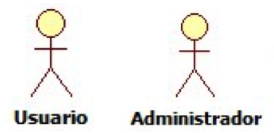
\includegraphics[width=0.5\textwidth]{Figuras/actores.png}
		\rule{30em}{0.5pt}
	\caption[Actores de TASMC]{Actores de TASMC}
	\label{fig:actoresTASMC}
\end{figure}
\clearpage

\begin{table}[htbp]
	\begin{center}
		\begin{tabular}{|p{2.5cm}|p{6.4cm}|p{2cm}|p{2cm}|}
			\hline
				\rowcolor[RGB]{51,153,255}{Actor}&\multicolumn{2}{c}{Usuario}&{\textbf{ACT-01}}\\
			\hline
				{Descripción}&\multicolumn{3}{p{11.2cm}|}{
			Es el actor principal y por lo tanto tiene la mayor interacción con el sistema. El usuario hace uso de todos 				los servicios proporcionados por la aplicación, es decir, configuración de viaje dependiendo de gustos y 					posibilidades, consultar sugerencias de vuelos y hoteles, control de equipaje, uso de itinerario de viaje, la 				creación de ruta casa-aeropuerto, localización dentro del AICM y visualizar estado de vuelo.}\\
			\hline
				{Características}&\multicolumn{3}{p{11.2cm}|}{Actor Primario}\\
			\hline
				{Referencias}&\multicolumn{3}{p{11.2cm}|}{Caso de Uso General}\\
			\hline
				{Autor}&{Vivanco Carmona Erick Rafael}&{\textbf{Fecha} 09/01/15}&{\textbf{Versión} 2.0}\\
			\hline
				{Evaluador}&{Barajas Uribe Sergio}&{\textbf{Fecha} 15/01/15}&{\textbf{Estatus} Aprobado}\\
			\hline
				{Comentarios}&\multicolumn{3}{p{11.2cm}|}{Al ser el actor principal, la funcionalidad de la aplicación 						únicamente cobra sentido cuando el usuario inicia la aplicación y hace uso de los servicios 										proporcionados por el sistema.}\\
			\hline
		\end{tabular}
	\end{center}
	\caption[Descripción del Perfil del Actor Usuario]{Descripción del Perfil del Actor Usuario}
    	\label{tab:perfilUsuario}
\end{table}

\begin{table}[htbp]
	\begin{center}
		\begin{tabular}{|p{2.5cm}|p{6.4cm}|p{2cm}|p{2cm}|}
			\hline
				\rowcolor[RGB]{51,153,255}{Actor}&\multicolumn{2}{c}{Administrador}&{\textbf{ACT-02}}\\
			\hline
				{Descripción}&\multicolumn{3}{p{11.2cm}|}{
			Es el encargado de gestionar los elementos de hardware y software del sistema (Base de datos, Servidor y Web Service).}\\
			\hline
				{Características}&\multicolumn{3}{p{11.2cm}|}{Actor Secundario}\\
			\hline
				{Referencias}&\multicolumn{3}{p{11.2cm}|}{Caso de Uso General}\\
			\hline
				{Autor}&{Vivanco Carmona Erick Rafael}&{\textbf{Fecha} 09/01/15}&{\textbf{Versión} 2.0}\\
			\hline
				{Evaluador}&{Barajas Uribe Sergio}&{\textbf{Fecha} 15/01/15}&{\textbf{Estatus} Aprobado}\\
			\hline
				{Comentarios}&\multicolumn{3}{p{11.2cm}|}{Sin la gestión que realiza este actor al sistema no puede dar la funcionalidad necesaria para proporcionar al usuario los beneficios de la aplicación.}\\
			\hline
		\end{tabular}
	\end{center}
	\caption[Descripción del Perfil del Actor Administrador]{Descripción del Perfil del Actor Administrador}
    	\label{tab:perfilAdministrador}
\end{table}
\clearpage
\section{Casos de Uso del Administrador}

\subsection{Diagrama de Casos de Uso General del Administrador}

\begin{figure}[htbp]
	\centering
		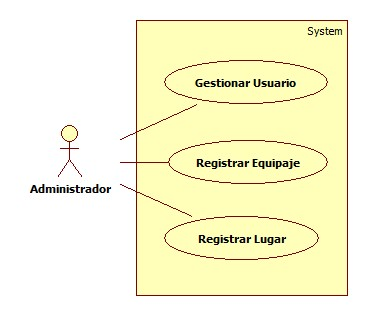
\includegraphics[width=0.4\textwidth]{Figuras/cugeneralAdministrador.png}
		\rule{30em}{0.5pt}
	\caption[Diagrama de Casos de Uso General del Administrador]{Diagrama de Casos de Uso General del Administrador}
	\label{fig:cuGeneralAdministrador}
\end{figure}

\subsection{Caso de Uso Gestionar Usuario}

\begin{figure}[htbp]
	\centering
		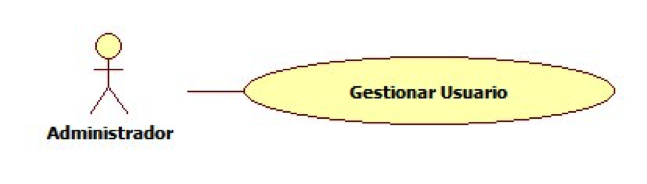
\includegraphics[width=0.9\textwidth]{Figuras/cuGestionarUsuario.png}
		\rule{30em}{0.5pt}
	\caption[Diagrama de Caso de Uso Gestionar Usuario]{Diagrama de Caso de Uso Gestionar Usuario}
	\label{fig:cuGestionarUsuario}
\end{figure}

\begin{longtable}{|p{2.5cm}|p{6.4cm}|p{2cm}|p{2cm}|}
	\hline
		\rowcolor[RGB]{255,102,102}{Caso de Uso}&\multicolumn{2}{c}{Gestionar Usuario}&{\textbf{CU-A-01}}\\
	\hline
		{Actores}&\multicolumn{3}{p{11.2cm}|}{Administrador}\\
	\hline
		{Tipo}&\multicolumn{3}{p{11.2cm}|}{Esencial}\\
	\hline
		{Precondición}&\multicolumn{3}{p{11.2cm}|}{El administrador se autentifica en el sistema.}\\
	\hline
		{Postcondición}&\multicolumn{3}{p{11.2cm}|}{Haber eliminado usuarios inactivos del sistema.}\\
	\hline
		{Autor}&{Vivanco Carmona Erick Rafael}&{\textbf{Fecha} 09/01/15}&{\textbf{Versión} 2.0}\\
			\hline
		{Evaluador}&{Barajas Uribe Sergio}&{\textbf{Fecha} 15/01/15}&{\textbf{Estatus} Aprobado}\\
	\hline
		{Propósito}&\multicolumn{3}{p{11.2cm}|}{Eliminar usuarios del sistema que hayan estado inactivos por mucho tiempo, de esta manera se tendrá un mayor control del número de usuarios del sistema.}\\
	\hline
		{Resumen}&\multicolumn{3}{p{11.2cm}|}{El administrador identifica usuarios inactivos y los da de baja.}\\	
	\hline
	\caption[Especificación del Caso de Uso Gestionar Usuario]{Especificación del Caso de Uso Gestionar Usuario}
    	\label{tab:cuGestionarUsuario}
\end{longtable}

\begin{flushleft}
	\textbf{Trayectoria Principal}\\
	\begin{enumerate}
		\item El administrador solicita la lista de usuarios.
		\item El sistema despliega los usuarios.
		\item El administrador identifica usuarios inactivos y los da de baja.
	\end{enumerate}
\end{flushleft}
----Fin del caso de uso

\subsection{Caso de Uso Registrar Equipaje}

\begin{figure}[htbp]
	\centering
		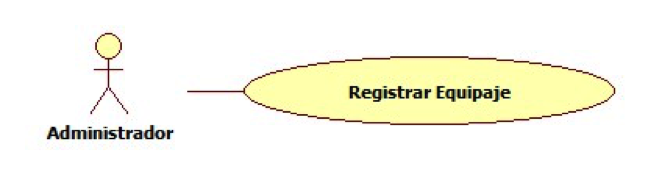
\includegraphics[width=0.9\textwidth]{Figuras/cuRegistrarEquipaje.png}
		\rule{30em}{0.5pt}
	\caption[Diagrama de Caso de Uso Registrar Equipaje]{Diagrama de Caso de Uso Registrar Equipaje}
	\label{fig:cuRegistrarEquipaje}
\end{figure}

\begin{longtable}{|p{2.5cm}|p{6.4cm}|p{2cm}|p{2cm}|}
	\hline
		\rowcolor[RGB]{255,102,102}{Caso de Uso}&\multicolumn{2}{c}{Registrar Equipaje}&{\textbf{CU-A-02}}\\
	\hline
		{Actores}&\multicolumn{3}{p{11.2cm}|}{Administrador}\\
	\hline
		{Tipo}&\multicolumn{3}{p{11.2cm}|}{Esencial}\\
	\hline
		{Precondición}&\multicolumn{3}{p{11.2cm}|}{El administrador se autentifica en el sistema.}\\
	\hline
		{Postcondición}&\multicolumn{3}{p{11.2cm}|}{Registrar objetos para equipaje.}\\
	\hline
		{Autor}&{Vivanco Carmona Erick Rafael}&{\textbf{Fecha} 09/01/15}&{\textbf{Versión} 2.0}\\
			\hline
		{Evaluador}&{Barajas Uribe Sergio}&{\textbf{Fecha} 15/01/15}&{\textbf{Estatus} Aprobado}\\
	\hline
		{Propósito}&\multicolumn{3}{p{11.2cm}|}{Registrar objetos útiles para un equipaje de viaje.}\\
	\hline
		{Resumen}&\multicolumn{3}{p{11.2cm}|}{El administrador registra y elimina objetos que puedan ser útiles para el usuario al momento de generar un equipaje para su viaje.}\\	
	\hline
	\caption[Especificación del Caso de Uso Registrar Equipaje]{Especificación del Caso de Uso Registrar Equipaje}
    	\label{tab:cuRegistrarEquipaje}
\end{longtable}

\begin{flushleft}
	\textbf{Trayectoria Principal}\\
	\begin{enumerate}
		\item El administrador solicita registrar equipaje.
		\item El administrador registra objetos. \hyperlink{TrayectoriaA_CU-A-02}{[Trayectoria A]}.
		\item Los objetos quedan disponibles para futuras listas de equipaje que el usuario desee crear.
		\item El administrador elimina objetos.
	\end{enumerate}
\end{flushleft}
----Fin del caso de uso

\begin{flushleft}
	\hypertarget{TrayectoriaA_CU-A-02}{}
	\textbf{Trayectoria Alternativa A}\\
	\textbf{Condición:} El administrador ha registrado un objeto. \\
	\begin{enumerate}
		\item El objeto ha sido creado y se notifica al administrador. 
		\item Volver a 2.
	\end{enumerate}
\end{flushleft}
----Fin de Trayectoria

\subsection{Caso de Uso Gestionar Lugar}

\begin{figure}[htbp]
	\centering
		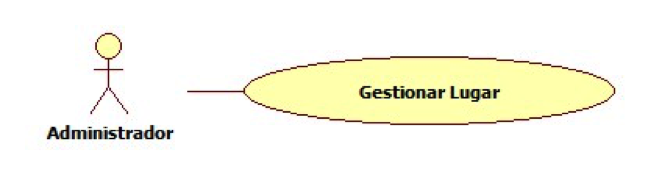
\includegraphics[width=0.9\textwidth]{Figuras/cuGestionarLugar.png}
		\rule{30em}{0.5pt}
	\caption[Diagrama de Caso de Uso Gestionar Lugar]{Diagrama de Caso de Uso Gestionar Lugar}
	\label{fig:cuGestionarLugar}
\end{figure}

\begin{longtable}{|p{2.5cm}|p{6.4cm}|p{2cm}|p{2cm}|}
	\hline
		\rowcolor[RGB]{255,102,102}{Caso de Uso}&\multicolumn{2}{c}{Gestionar Lugar}&{\textbf{CU-A-03}}\\
	\hline
		{Actores}&\multicolumn{3}{p{11.2cm}|}{Administrador}\\
	\hline
		{Tipo}&\multicolumn{3}{p{11.2cm}|}{Esencial}\\
	\hline
		{Precondición}&\multicolumn{3}{p{11.2cm}|}{El administrador se autentifica en el sistema.}\\
	\hline
		{Postcondición}&\multicolumn{3}{p{11.2cm}|}{Registrar lugares en el sistema.}\\
	\hline
		{Autor}&{Vivanco Carmona Erick Rafael}&{\textbf{Fecha} 09/01/15}&{\textbf{Versión} 2.0}\\
			\hline
		{Evaluador}&{Barajas Uribe Sergio}&{\textbf{Fecha} 15/01/15}&{\textbf{Estatus} Aprobado}\\
	\hline
		{Propósito}&\multicolumn{3}{p{11.2cm}|}{Registrar lugares del AICM para que el usuario pueda visualizarlos en su localización dentro del AICM.}\\
	\hline
		{Resumen}&\multicolumn{3}{p{11.2cm}|}{El administrador registra lugares del AICM.}\\	
	\hline
	\caption[Especificación del Caso de Uso Gestionar Lugar]{Especificación del Caso de Uso Gestionar Lugar}
    	\label{tab:cuGestionarLugar}
\end{longtable}
\newpage
\begin{flushleft}
	\textbf{Trayectoria Principal}\\
	\begin{enumerate}
		\item El administrador desea gestionar lugares en el AICM.
		\item El administrador da de alta un lugar en una determinada coordenada en el AICM.
		\item El lugar (servicio) queda registrado en el sistema, para posterior uso en la localización del usuario dentro del AICM.
		\item El administrador da de baja un lugar del AICM.
	\end{enumerate}
\end{flushleft}
----Fin del caso de uso
\section{Casos de Uso del Usuario}

\subsection{Diagrama de Casos de Uso General del Usuario}

\begin{figure}[htbp]
	\centering
		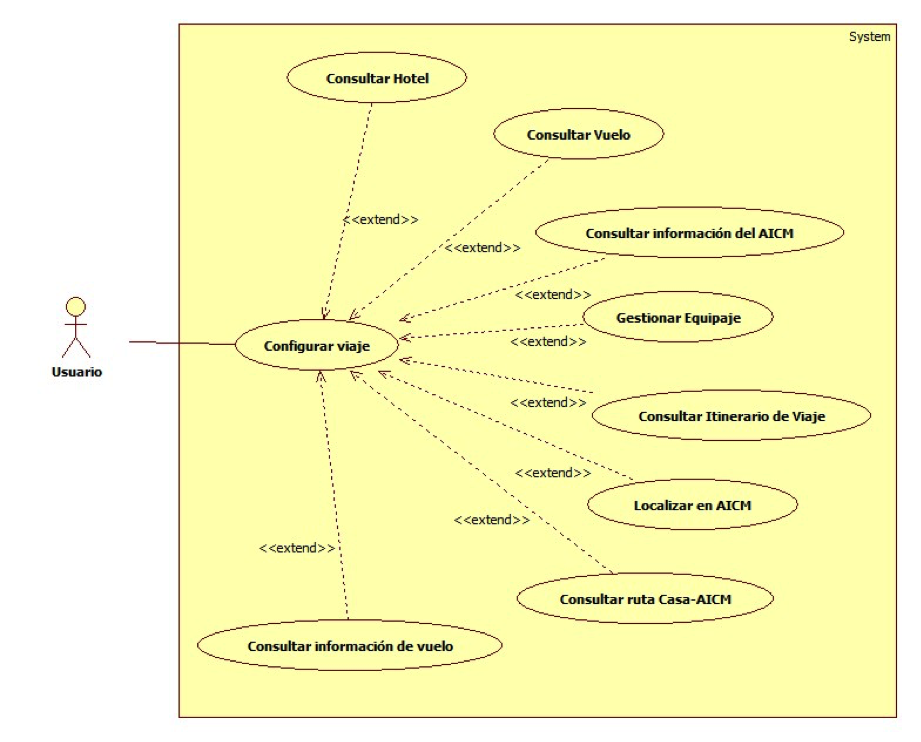
\includegraphics[width=0.9\textwidth]{Figuras/cugeneralUsuario.png}
		\rule{30em}{0.5pt}
	\caption[Diagrama de Casos de Uso General del Usuario]{Diagrama de Casos de Uso General del Usuario}
	\label{fig:cuGeneralUsuario}
\end{figure}

\subsection{Caso de Uso Configurar Viaje}

\begin{figure}[htbp]
	\centering
		
\includegraphics[width=0.9\textwidth]{Figuras/cuConfigurarViaje.png}
		\rule{30em}{0.5pt}
	\caption[Diagrama de Caso de Uso Configurar Viaje]{Diagrama de Caso de Uso Configurar Viaje}
	\label{fig:cuConfigurarViaje}
\end{figure}

\begin{longtable}[h]{|p{2.5cm}|p{6.4cm}|p{2cm}|p{2cm}|}
	\hline
		\rowcolor[RGB]{51,153,255}{Caso de Uso}&\multicolumn{2}{c}{Configurar Viaje}&{\textbf{CU-U-01}}\\
	\hline
		{Actores}&\multicolumn{3}{p{11.2cm}|}{Usuario}\\
	\hline
		{Tipo}&\multicolumn{3}{p{11.2cm}|}{Esencial}\\
	\hline
		{Precondición}&\multicolumn{3}{p{11.2cm}|}{El usuario puede o no realizar su configuración de viaje, pero la aplicación le hará la sugerencia de realizarla en otro momento.}\\
	\hline
		{Postcondición}&\multicolumn{3}{p{11.2cm}|}{La configuración del usuario ha quedado registrada, por lo tanto, está en condiciones de hacer uso de los servicios ofrecidos por el sistema.}\\
	\hline
		{Autor}&{Vivanco Carmona Erick Rafael}&{\textbf{Fecha} 09/01/15}&{\textbf{Versión} 2.0}\\
			\hline
		{Evaluador}&{Barajas Uribe Sergio}&{\textbf{Fecha} 15/01/15}&{\textbf{Estatus} Aprobado}\\
	\hline
		{Propósito}&\multicolumn{3}{p{11.2cm}|}{Configurar sus viajes dependiendo de la clase de viaje que más le agrade al usuario y la categoría de hoteles que frecuenta.}\\
	\hline
		{Resumen}&\multicolumn{3}{p{11.2cm}|}{El usuario realiza la configuración de la aplicación según la clase en la que más le gusta viajar y la categoría de hoteles que desea el usuario además proporciona su correo electrónico para tener el control de su usuario.}\\	
	\hline
		{Comentarios}&\multicolumn{3}{p{11.2cm}|}{Los datos guardados estarán protegidos y únicamente se enviaran notificaciones acerca de la aplicación al correo proporcionado.}\\	
	\hline
	\caption[Especificación del Caso de Uso Configurar Viaje]{Especificación del Caso de Uso Configurar Viaje}
    	\label{tab:cuConfigurarViaje}
\end{longtable}
\newpage
\begin{flushleft}
	\textbf{Trayectoria Principal}\\
	\begin{enumerate}
		\item El usuario inicia la aplicación por primera vez e inmediatamente se le indica si gusta configurar su aplicación con la clase en la que le guste viajar y categoría de hotel que prefiere. \hyperlink{TrayectoriaA_CU-U-01}{[Trayectoria A]}.
		\item El sistema presenta un formulario para que el usuario introduzca su correo electrónico, la clase de viaje y categoría de hotel.
		\item El usuario introduce los datos y los envía para que sean registrados.
		\item El sistema válida la configuración proporcionada por el usuario. \hyperlink{TrayectoriaB_CU-U-01}{[Trayectoria B]}.
		\item La configuración del usuario queda registrada en el sistema. Se notifica al usuario.
	\end{enumerate}
\end{flushleft}
----Fin del caso de uso

\begin{flushleft}
	\hypertarget{TrayectoriaA_CU-U-01}{}
	\textbf{Trayectoria Alternativa A}\\
	\textbf{Condición:} La conexión con el servidor se pierde. \\
	\textbf{Nota: } Este curso alterno puede presentarse en cualquier momento durante el curso de CU-U-01.\\
	\begin{enumerate}
		\item El cliente debe reintentar completar la operación en otro momento. 
		\item Volver a 1. 
	\end{enumerate}
\end{flushleft}
----Fin de Trayectoria

\begin{flushleft}
	\hypertarget{TrayectoriaB_CU-U-01}{}
	\textbf{Trayectoria Alternativa B}\\
	\textbf{Condición:} La configuración no es correcta.  \\
	\begin{enumerate}
		\item Se notifica al usuario y se solicita que los datos erróneos sean modificados. 
		\item Volver a 2.
	\end{enumerate}
\end{flushleft}
----Fin de Trayectoria
\newpage
\subsection{Caso de Uso Consultar Hotel}

\begin{figure}[htbp]
	\centering
		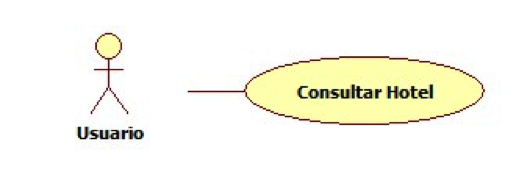
\includegraphics[width=0.9\textwidth]{Figuras/cuConsultarHotel.png}
		\rule{30em}{0.5pt}
	\caption[Diagrama de Caso de Uso Consultar Hotel]{Diagrama de Caso de Uso Consultar Hotel}
	\label{fig:cuConsultarHotel}
\end{figure}

\begin{longtable}{|p{2.5cm}|p{6.4cm}|p{2cm}|p{2cm}|}
	\hline
		\rowcolor[RGB]{51,153,255}{Caso de Uso}&\multicolumn{2}{c}{Consultar Hotel}&{\textbf{CU-U-02}}\\
	\hline
		{Actores}&\multicolumn{3}{p{11.2cm}|}{Usuario}\\
	\hline
		{Tipo}&\multicolumn{3}{p{11.2cm}|}{Esencial}\\
	\hline
		{Precondición}&\multicolumn{3}{p{11.2cm}|}{	Existen hoteles registrados en el Web Service.}\\
	\hline
		{Postcondición}&\multicolumn{3}{p{11.2cm}|}{El turista tiene a su disposición la información de hoteles acorde a sus posibilidades.}\\
	\hline
		{Autor}&{Vivanco Carmona Erick Rafael}&{\textbf{Fecha} 09/01/15}&{\textbf{Versión} 2.0}\\
			\hline
		{Evaluador}&{Barajas Uribe Sergio}&{\textbf{Fecha} 15/01/15}&{\textbf{Estatus} Aprobado}\\
	\hline
		{Propósito}&\multicolumn{3}{p{11.2cm}|}{Consultar información de hoteles.}\\
	\hline
		{Resumen}&\multicolumn{3}{p{11.2cm}|}{El usuario realiza una búsqueda de hoteles y se muestra un listado de los mismos según los parámetros de la búsqueda. }\\	
	\hline
	\caption[Especificación del Caso de Uso Consultar Hotel]{Especificación del Caso de Uso Consultar Hotel}
    	\label{tab:cuConsultarHotel}
\end{longtable}

\begin{flushleft}
	\textbf{Trayectoria Principal}\\
	\begin{enumerate}
		\item El usuario solicita consultar hoteles. \hyperlink{TrayectoriaA_CU-U-02}{[Trayectoria A]}.
		\item Se despliega un formulario para realizar la búsqueda según: ubicación del hotel o categoría del hotel.
		\item El usuario ingresa los parámetros de interés. \hyperlink{TrayectoriaB_CU-U-02}{[Trayectoria B]}.
		\item Se  muestra un listado de hoteles disponibles con las características requeridas. \hyperlink{TrayectoriaC_CU-U-02}{[Trayectoria C]}.
		\item El usuario puede realizar un filtrado de la lista por: estrellas de 1 a 5 o de 5 a 1; precios de bajo a alto o precios de alto a bajo.
		\item El usuario puede visualizar la información detallada de cada hotel.
	\end{enumerate}
\end{flushleft}
----Fin del caso de uso

\begin{flushleft}
	\hypertarget{TrayectoriaA_CU-U-02}{}
	\textbf{Trayectoria Alternativa A}\\
	\textbf{Condición:} La conexión con el servidor se pierde. \\
	\textbf{Nota: } Este curso alterno puede presentarse en cualquier momento durante el curso de CU-U-02. \\	
	\begin{enumerate}
		\item El cliente debe reintentar completar la operación en otro momento. 
		\item Volver a 1. 
	\end{enumerate}
\end{flushleft}
----Fin de Trayectoria

\begin{flushleft}
	\hypertarget{TrayectoriaB_CU-U-02}{}
	\textbf{Trayectoria Alternativa B}\\
	\textbf{Condición:} El usuario no ha ingresado los parámetros adecuados para la búsqueda. \\
	\begin{enumerate}
		\item  Se notifica al usuario y se solicita que indique los parámetros adecuados para la búsqueda.
	\end{enumerate}
\end{flushleft}
----Fin de Trayectoria

\begin{flushleft}
	\hypertarget{TrayectoriaC_CU-U-02}{}
	\textbf{Trayectoria Alternativa C}\\
	\textbf{Condición:} La búsqueda no obtiene resultados con las características requeridas. \\
	\begin{enumerate}
		\item Se despliega una notificación de aviso y se solicita iniciar una nueva búsqueda. 
		\item Volver a 1.
	\end{enumerate}
\end{flushleft}
----Fin de Trayectoria
\newpage
\subsection{Caso de Uso Consultar Vuelo}

\begin{figure}[htbp]
	\centering
		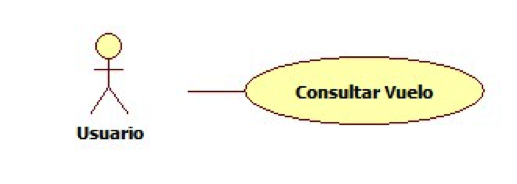
\includegraphics[width=0.9\textwidth]{Figuras/cuConsultarVuelo.png}
		\rule{30em}{0.5pt}
	\caption[Diagrama de Caso de Uso Consultar Vuelo]{Diagrama de Caso de Uso Consultar Vuelo}
	\label{fig:cuConsultarVuelo}
\end{figure}

\begin{longtable}{|p{2.5cm}|p{6.4cm}|p{2cm}|p{2cm}|}
	\hline
		\rowcolor[RGB]{51,153,255}{Caso de Uso}&\multicolumn{2}{c}{Consultar Vuelo}&{\textbf{CU-U-03}}\\
	\hline
		{Actores}&\multicolumn{3}{p{11.2cm}|}{Usuario}\\
	\hline
		{Tipo}&\multicolumn{3}{p{11.2cm}|}{Esencial}\\
	\hline
		{Precondición}&\multicolumn{3}{p{11.2cm}|}{Existen vuelos registrados en el Web Service.}\\
	\hline
		{Postcondición}&\multicolumn{3}{p{11.2cm}|}{El turista tiene a su disposición la información de hoteles acorde a sus posibilidades y configuración de viaje.}\\
	\hline
		{Autor}&{Vivanco Carmona Erick Rafael}&{\textbf{Fecha} 09/01/15}&{\textbf{Versión} 2.0}\\
			\hline
		{Evaluador}&{Barajas Uribe Sergio}&{\textbf{Fecha} 15/01/15}&{\textbf{Estatus} Aprobado}\\
	\hline
		{Propósito}&\multicolumn{3}{p{11.2cm}|}{Consultar información de vuelos.}\\
	\hline
		{Resumen}&\multicolumn{3}{p{11.2cm}|}{El usuario realiza una búsqueda de vuelos y se muestra un listado de los mismos según los parámetros de la búsqueda.}\\	
	\hline
		{Comentarios}&\multicolumn{3}{p{11.2cm}|}{Si el usuario ha realizado su configuración, la clase por defecto será la que el configuró.}\\	
	\hline
	\caption[Especificación del Caso de Uso Consultar Vuelo]{Especificación del Caso de Uso Consultar Vuelo}
    	\label{tab:cuConsultarVuelo}
\end{longtable}
\newpage
\begin{flushleft}
	\textbf{Trayectoria Principal}\\
	\begin{enumerate}
		\item El usuario solicita consultar vuelos. \hyperlink{TrayectoriaA_CU-U-03}{[Trayectoria A]}.
		\item Se despliega un formulario para realizar la búsqueda según: fechas (salida- regreso) o desde – a o clase (Económico, Económico Premium, Business, Primera, Todas).
		\item El usuario selecciona los parámetros de interés. \hyperlink{TrayectoriaB_CU-U-03}{[Trayectoria B]}.
		\item Se  muestra un listado de vuelos disponibles con las características requeridas. \hyperlink{TrayectoriaC_CU-U-03}{[Trayectoria C]}.
		\item El usuario puede realizar un filtrado de la lista por: clase o precios de bajo a alto o precios de alto a bajo.
		\item	El usuario puede visualizar la información detallada de cada vuelo.
	\end{enumerate}
\end{flushleft}
----Fin del caso de uso

\begin{flushleft}
	\hypertarget{TrayectoriaA_CU-U-03}{}
	\textbf{Trayectoria Alternativa A}\\
	\textbf{Condición:} La conexión con el servidor se pierde. \\
	\textbf{Nota: } Este curso alterno puede presentarse en cualquier momento durante el curso de CU-U-03. \\	
	\begin{enumerate}
		\item El cliente debe reintentar completar la operación en otro momento. 
		\item Volver a 1. 
	\end{enumerate}
\end{flushleft}
----Fin de Trayectoria

\begin{flushleft}
	\hypertarget{TrayectoriaB_CU-U-03}{}
	\textbf{Trayectoria Alternativa B}\\
	\textbf{Condición:} El usuario no ha ingresado los parámetros adecuados para la búsqueda. \\
	\begin{enumerate}
		\item  Se notifica al usuario y se solicita que indique los parámetros adecuados para la búsqueda.
	\end{enumerate}
\end{flushleft}
----Fin de Trayectoria

\begin{flushleft}
	\hypertarget{TrayectoriaC_CU-U-03}{}
	\textbf{Trayectoria Alternativa C}\\
	\textbf{Condición:} La búsqueda no obtiene resultados con las características requeridas. \\
	\begin{enumerate}
		\item Se despliega una notificación de aviso y se solicita iniciar una nueva búsqueda. 
		\item Volver a 1.
	\end{enumerate}
\end{flushleft}
----Fin de Trayectoria

\subsection{Caso de Uso Consultar Información AICM}

\begin{figure}[htbp]
	\centering
		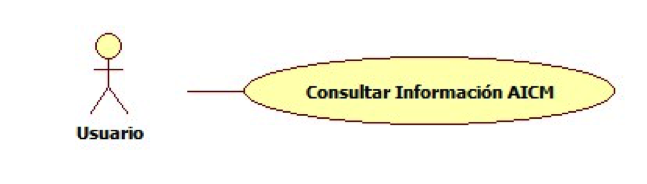
\includegraphics[width=0.9\textwidth]{Figuras/cuConsultarInformacionAICM.png}
		\rule{30em}{0.5pt}
	\caption[Diagrama de Caso de Uso Consultar Informacion AICM]{Diagrama de Caso de Uso Consultar Informacion AICM}
	\label{fig:cuConsultarInformacionAICM}
\end{figure}

\begin{longtable}{|p{2.5cm}|p{6.4cm}|p{2cm}|p{2cm}|}
	\hline
		\rowcolor[RGB]{51,153,255}{Caso de Uso}&\multicolumn{2}{c}{Consultar Información AICM}&{\textbf{CU-U-04}}\\
	\hline
		{Actores}&\multicolumn{3}{p{11.2cm}|}{Usuario}\\
	\hline
		{Tipo}&\multicolumn{3}{p{11.2cm}|}{Esencial}\\
	\hline
		{Precondición}&\multicolumn{3}{p{11.2cm}|}{El administrador ha registrado en el sistema la información del AICM.}\\
	\hline
		{Postcondición}&\multicolumn{3}{p{11.2cm}|}{El usuario tiene a su disposición la información sobre el AICM.}\\
	\hline
		{Autor}&{Vivanco Carmona Erick Rafael}&{\textbf{Fecha} 09/01/15}&{\textbf{Versión} 2.0}\\
			\hline
		{Evaluador}&{Barajas Uribe Sergio}&{\textbf{Fecha} 15/01/15}&{\textbf{Estatus} Aprobado}\\
	\hline
		{Propósito}&\multicolumn{3}{p{11.2cm}|}{Consultar la información relacionada con el AICM como es el teléfono del aeropuerto para consultar alguna duda, ubicación, servicios y página web.}\\
	\hline
		{Resumen}&\multicolumn{3}{p{11.2cm}|}{El usuario consulta la información del AICM que previamente ha sido registrada por el administrador y se encuentra disponible en la aplicación.}\\	
	\hline
	\caption[Especificación del Caso de Uso Consultar Información AICM]{Especificación del Caso de Uso Consultar Información AICM}
    	\label{tab:cuConsultarInformacionAICM}
\end{longtable}

\begin{flushleft}
	\textbf{Trayectoria Principal}\\
	\begin{enumerate}
		\item El usuario solicita la información del AICM. \hyperlink{TrayectoriaA_CU-U-04}{[Trayectoria A]}.
		\item Se despliega la información del AICM.
	\end{enumerate}
\end{flushleft}
----Fin del caso de uso

\begin{flushleft}
	\hypertarget{TrayectoriaA_CU-U-04}{}
	\textbf{Trayectoria Alternativa A}\\
	\textbf{Condición:} No existe información registrada o disponible en el sistema. \\
	\begin{enumerate}
		\item  Se notifica al turista. 
		\item Termina la operación.
	\end{enumerate}
\end{flushleft}
----Fin de Trayectoria
\subsection{Caso de Uso Gestionar Equipaje}

\begin{figure}[htbp]
	\centering
		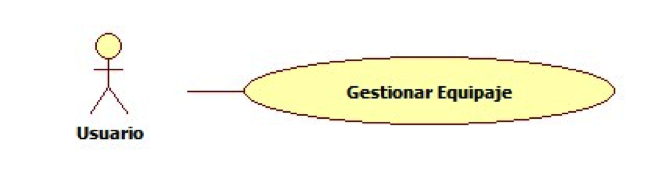
\includegraphics[width=0.9\textwidth]{Figuras/cuGestionarEquipajeU.png}
		\rule{30em}{0.5pt}
	\caption[Diagrama de Caso de Uso Gestionar Equipaje]{Diagrama de Caso de Uso Gestionar Equipaje}
	\label{fig:cuGestionarEquipajeU}
\end{figure}
\newpage
\begin{longtable}[h!]{|p{2.5cm}|p{6.4cm}|p{2cm}|p{2cm}|}
	\hline
		\rowcolor[RGB]{51,153,255}{Caso de Uso}&\multicolumn{2}{c}{Gestionar Equipaje}&{\textbf{CU-U-05}}\\
	\hline
		{Actores}&\multicolumn{3}{p{11.2cm}|}{Usuario}\\
	\hline
		{Tipo}&\multicolumn{3}{p{11.2cm}|}{Esencial}\\
	\hline
		{Precondición}&\multicolumn{3}{p{11.2cm}|}{El administrador ha registrado objetos de viaje.}\\
	\hline
		{Postcondición}&\multicolumn{3}{p{11.2cm}|}{El usuario tiene a su disposición objetos para crear lista de equipaje.}\\
	\hline
		{Autor}&{Vivanco Carmona Erick Rafael}&{\textbf{Fecha} 09/01/15}&{\textbf{Versión} 2.0}\\
			\hline
		{Evaluador}&{Barajas Uribe Sergio}&{\textbf{Fecha} 15/01/15}&{\textbf{Estatus} Aprobado}\\
	\hline
		{Propósito}&\multicolumn{3}{p{11.2cm}|}{Consultar el equipaje del usuario necesario para su viaje.}\\
	\hline
		{Resumen}&\multicolumn{3}{p{11.2cm}|}{El usuario selecciona objetos dependiendo del tipo de viaje que vaya a realizar y consulta los objetos seleccionados para su comprobación.}\\	
	\hline
		{Comentarios}&\multicolumn{3}{p{11.2cm}|}{Existen equipajes predeterminados, pero el usuario puede crear el suyo personalizado.}\\
	\hline
	\caption[Especificación del Caso de Uso Gestionar Equipaje]{Especificación del Caso de Uso Gestionar Equipaje}
    	\label{tab:cuGestionarEquipajeU}
\end{longtable}

\begin{flushleft}
	\textbf{Trayectoria Principal}\\
	\begin{enumerate}
		\item El usuario solicita crear lista de equipaje.
		\item Se solicita el nombre de la categoría de viaje.
		\item Se solicita los objetos requeridos para la lista de equipaje.
		\item Se crea la lista de equipaje.
		\item El usuario solicita verificar su equipaje.
		\item Se despliegan los objetos registrados en la lista de equipaje.
		\item El usuario verifica los objetos.
		\item El usuario edita lista de equipaje.
		\item El usuario añade objetos a la lista de equipaje.
	\end{enumerate}
\end{flushleft}
----Fin del caso de uso

\subsection{Caso de Uso Consultar Itinerario de Viaje}
\hypertarget{CU-U-06}{}

\begin{figure}[htbp]
	\centering
		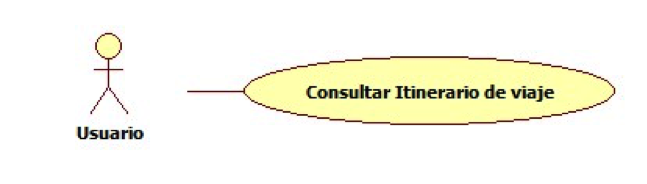
\includegraphics[width=0.9\textwidth]{Figuras/cuConsultarItinerarioViaje.png}
		\rule{30em}{0.5pt}
	\caption[Diagrama de Caso de Uso Consultar Itinerario de Viaje]{Diagrama de Caso de Uso Consultar Itinerario de Viaje}
	\label{fig:cuConsultarItinerarioViaje}
\end{figure}

\begin{longtable}{|p{2.5cm}|p{6.4cm}|p{2cm}|p{2cm}|}
	\hline
		\rowcolor[RGB]{51,153,255}{Caso de Uso}&\multicolumn{2}{c}{Consultar Itinerario de Viaje}&{\textbf{CU-U-06}}\\
	\hline
		{Actores}&\multicolumn{3}{p{11.2cm}|}{Usuario}\\
	\hline
		{Tipo}&\multicolumn{3}{p{11.2cm}|}{Esencial}\\
	\hline
		{Precondición}&\multicolumn{3}{p{11.2cm}|}{El usuario debe registrar el número de vuelo, el tipo de vuelo y la lista de actividades que realizará en el viaje.}\\
	\hline
		{Postcondición}&\multicolumn{3}{p{11.2cm}|}{El usuario tiene a su disposición la información de su vuelo, una alarma programada según el tipo viaje del usuario y un itinerario de su viaje.}\\
	\hline
		{Autor}&{Vivanco Carmona Erick Rafael}&{\textbf{Fecha} 09/01/15}&{\textbf{Versión} 2.0}\\
			\hline
		{Evaluador}&{Barajas Uribe Sergio}&{\textbf{Fecha} 15/01/15}&{\textbf{Estatus} Aprobado}\\
	\hline
		{Propósito}&\multicolumn{3}{p{11.2cm}|}{Consultar la información relacionada con su vuelo y organizar el tiempo del usuario para llegar a tiempo a su vuelo en el AICM, además de visualizar el itinerario de viaje del usuario.}\\
	\hline
		{Resumen}&\multicolumn{3}{p{11.2cm}|}{El usuario obtiene la información de su vuelo, itinerario de viaje que haya descrito previamente, se programa una alarma en el dispositivo móvil del usuario tomando en cuenta la hora de salida y el tipo de vuelo ya sea nacional la alarma se programara 3.5 horas antes e internacional 4.5 horas antes.}\\	
	\hline
		{Comentarios}&\multicolumn{3}{p{11.2cm}|}{La alarma solo podrá ser programada hasta que el usuario ingrese el tipo de vuelo, así como el itinerario que se muestre será a partir de las actividades que el usuario ingrese.}\\	
	\hline
	\caption[Especificación del Caso de Uso Consultar Itinerario de Viaje]{Especificación del Caso de Uso Consultar Itinerario de Viaje}
    	\label{tab:cuConsultarItinerarioViaje}
\end{longtable}
\newpage
\begin{flushleft}
	\textbf{Trayectoria Principal}\\
	\begin{enumerate}
		\item El usuario solicita consultar un itinerario. \hyperlink{TrayectoriaA_CU-U-06}{[Trayectoria A]}.
		\item El usuario selecciona itinerario de viaje. 
		\item El sistema solicita el  número y tipo de vuelo.
		\item El sistema valida los datos proporcionados. No permitirá avanzar si no se ingresa el número y tipo de vuelo.
		\item El sistema despliega la información de vuelo y el itinerario de viaje. \hyperlink{TrayectoriaB_CU-U-06}{[Trayectoria B]}.
		\item El sistema programa una alarma a partir de la hora de salida del vuelo y el tipo de vuelo ya se internacional con 4.5 horas antes de la salida o nacional 3.5 horas antes.
		\item El usuario solicita itinerario de viaje.
		\item	El sistema solicita una lista de actividades que el usuario gusta realizar en su viaje (itinerario).
		\item Se despliega actividades para viaje.
		\item El usuario puede gestionar su itinerario modificando, agregando o eliminando actividades.
		\item El usuario puede modificar la alarma si así lo desea.
	\end{enumerate}
\end{flushleft}
----Fin del caso de uso

\begin{flushleft}
	\hypertarget{TrayectoriaA_CU-U-06}{}
	\textbf{Trayectoria Alternativa A}\\
	\textbf{Condición:} El usuario no ha registrado itinerario\\
	\begin{enumerate}
		\item El usuario no puede consultar itinerario si aun no ha registrado alguno.
	\end{enumerate}
\end{flushleft}
----Fin de Trayectoria

\begin{flushleft}
	\hypertarget{TrayectoriaB_CU-U-06}{}
	\textbf{Trayectoria Alternativa B}\\
	\textbf{Condición:} La conexión con el servidor se pierde. \\
	\begin{enumerate}
		\item Los datos del vuelo no pueden ser cargados correctamente. 
		\item El cliente debe reintentar completar la operación en otro momento. 
		\item Volver a 2. 
	\end{enumerate}
\end{flushleft}
----Fin de Trayectoria


\subsection{Caso de Uso Consultar Ruta casa-AICM}

\begin{figure}[htbp]
	\centering
		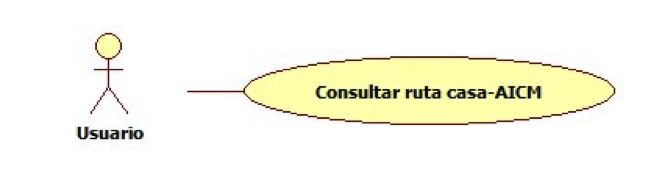
\includegraphics[width=0.9\textwidth]{Figuras/cuConsultarRutacasa-AICM.png}
		\rule{30em}{0.5pt}
	\caption[Diagrama de Caso de Uso Consultar Ruta casa-AICM]{Diagrama de Caso de Uso Consultar Ruta casa-AICM}
	\label{fig:cuConsultarRutacasa-AICM}
\end{figure}

\begin{longtable}{|p{2.5cm}|p{6.4cm}|p{2cm}|p{2cm}|}
	\hline
		\rowcolor[RGB]{51,153,255}{Caso de Uso}&\multicolumn{2}{c}{Consultar Ruta casa-AICM}&{\textbf{CU-U-07}}\\
	\hline
		{Actores}&\multicolumn{3}{p{11.2cm}|}{Usuario}\\
	\hline
		{Tipo}&\multicolumn{3}{p{11.2cm}|}{Esencial}\\
	\hline
		{Precondición}&\multicolumn{3}{p{11.2cm}|}{El usuario deberá estar conectado a una red de internet para generar la ruta de su origen al aeropuerto.}\\
	\hline
		{Postcondición}&\multicolumn{3}{p{11.2cm}|}{Se obtiene la ruta desde el punto de origen hacia el AICM.}\\
	\hline
		{Autor}&{Vivanco Carmona Erick Rafael}&{\textbf{Fecha} 09/01/15}&{\textbf{Versión} 2.0}\\
			\hline
		{Evaluador}&{Barajas Uribe Sergio}&{\textbf{Fecha} 15/01/15}&{\textbf{Estatus} Aprobado}\\
	\hline
		{Propósito}&\multicolumn{3}{p{11.2cm}|}{Obtener la ruta desde el origen del usuario al AICM.}\\
	\hline
		{Resumen}&\multicolumn{3}{p{11.2cm}|}{El usuario desea conocer cuál es la ruta para llegar al AICM desde su punto de origen. Por lo tanto, solicita dicha función al sistema, el sistema obtiene la ubicación actual del usuario y  genera la ruta hacia el AICM.}\\	
	\hline
		{Comentarios}&\multicolumn{3}{p{11.2cm}|}{El usuario debe estar conecta a una red para generar la ruta.}\\
	\hline
	\caption[Especificación del Caso de Uso Consultar Ruta casa-AICM]{Especificación del Caso de Uso Consultar Ruta casa-AICM}
    	\label{tab:cuConsultarRutacasa-AICM}
\end{longtable}

\begin{flushleft}
	\textbf{Trayectoria Principal}\\
	\begin{enumerate}
		\item El usuario solicita generar una nueva ruta casa-AICM. \hyperlink{TrayectoriaA_CU-U-07}{[Trayectoria A]}.
		\item Se obtiene la ubicación actual del usuario y se genera la ruta hacia el AICM.
		\item El usuario tiene a su disposición la ruta sugerida por el sistema para llegar desde su ubicación actual hacia el AICM.
	\end{enumerate}
\end{flushleft}
----Fin del caso de uso

\begin{flushleft}
	\hypertarget{TrayectoriaA_CU-U-07}{}
	\textbf{Trayectoria Alternativa A}\\
	\textbf{Condición:} No existe conexión con una red para generar la ruta. \\
	\begin{enumerate}
		\item Se solicita al usuario que se conecte a una red para generar la ruta. 
		\item Volver a 1.
	\end{enumerate}
\end{flushleft}
----Fin de Trayectoria

\subsection{Caso de Uso Ubicar en AICM}

\begin{figure}[htbp]
	\centering
		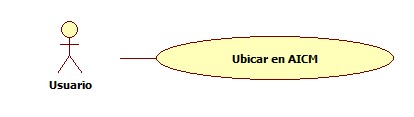
\includegraphics[width=0.9\textwidth]{Figuras/cuUbicarAICM.jpg}
		\rule{30em}{0.5pt}
	\caption[Diagrama de Caso de Uso Ubicar en AICM]{Diagrama de Caso de Uso Ubicar en AICM}
	\label{fig:cuUbicarAICM}
\end{figure}
\newpage
\begin{longtable}{|p{2.5cm}|p{6.4cm}|p{2cm}|p{2cm}|}
	\hline
		\rowcolor[RGB]{51,153,255}{Caso de Uso}&\multicolumn{2}{c}{Ubicar en AICM}&{\textbf{CU-U-08}}\\
	\hline
		{Actores}&\multicolumn{3}{p{11.2cm}|}{Usuario}\\
	\hline
		{Tipo}&\multicolumn{3}{p{11.2cm}|}{Esencial}\\
	\hline
		{Precondición}&\multicolumn{3}{p{11.2cm}|}{El sistema deberá estar entrenado en el AICM, y las salas de abordaje estarán previamente registradas.}\\
	\hline
		{Postcondición}&\multicolumn{3}{p{11.2cm}|}{Se obtiene la localización del usuario dentro del AICM.}\\
	\hline
		{Autor}&{Vivanco Carmona Erick Rafael}&{\textbf{Fecha} 09/01/15}&{\textbf{Versión} 2.0}\\
			\hline
		{Evaluador}&{Barajas Uribe Sergio}&{\textbf{Fecha} 15/01/15}&{\textbf{Estatus} Aprobado}\\
	\hline
		{Propósito}&\multicolumn{3}{p{11.2cm}|}{Obtener la ubicación del usuario dentro del AICM mediante el magnetómetro integrado en el dispositivo móvil, así como localizar la sala de abordaje y servicios en el AICM. }\\
	\hline
		{Resumen}&\multicolumn{3}{p{11.2cm}|}{El usuario solicita explorar el AICM, el sistema despliega la sala de abordaje que el usuario haya proporcionado y visualiza los servicios en el interior del AICM.}\\	
	\hline
		{Comentarios}&\multicolumn{3}{p{11.2cm}|}{El sistema deberá estar entrenado, de lo contrario, la ubicación será ineficiente.}\\
	\hline
	\caption[Especificación del Caso de Uso Ubicar en AICM]{Especificación del Caso de Uso Ubicar en AICM}
    	\label{tab:cuUbicarAICM}
\end{longtable}

\begin{flushleft}
	\textbf{Trayectoria Principal}\\
	\begin{enumerate}
		\item El turista solicita localizarse en el AICM.
		\item El sistema despliega un mapa del AICM donde se puede ubicar al usuario así como su sala de abordaje y servicios disponibles.
		\item El usuario tiene a su disposición el mapa el cual le mostrar su ubicación actual y permitirá desplazarse con mayor facilidad dentro del AICM.
	\end{enumerate}
\end{flushleft}
----Fin del caso de uso
\newpage
\subsection{Caso de Uso Consultar Información de Vuelo}

\begin{figure}[htbp]
	\centering
		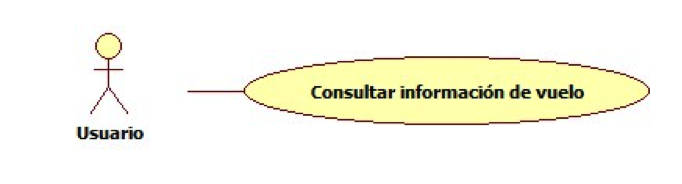
\includegraphics[width=0.9\textwidth]{Figuras/cuConsultarInformacionVuelo.png}
		\rule{30em}{0.5pt}
	\caption[Diagrama de Caso de Uso Consultar Información de Vuelo]{Diagrama de Caso de Uso Consultar Información de Vuelo}
	\label{fig:cuConsultarInformacionVuelo}
\end{figure}

\begin{longtable}{|p{2.5cm}|p{6.4cm}|p{2cm}|p{2cm}|}
	\hline
		\rowcolor[RGB]{51,153,255}{Caso de Uso}&\multicolumn{2}{c}{Consultar Información de Vuelo}&{\textbf{CU-U-09}}\\
	\hline
		{Actores}&\multicolumn{3}{p{11.2cm}|}{Usuario}\\
	\hline
		{Tipo}&\multicolumn{3}{p{11.2cm}|}{Esencial}\\
	\hline
		{Precondición}&\multicolumn{3}{p{11.2cm}|}{	El usuario ha registrado su número de vuelo.}\\
	\hline
		{Postcondición}&\multicolumn{3}{p{11.2cm}|}{El usuario tendrá a su disposición la información de su vuelo.}\\
	\hline
		{Autor}&{Vivanco Carmona Erick Rafael}&{\textbf{Fecha} 09/01/15}&{\textbf{Versión} 2.0}\\
			\hline
		{Evaluador}&{Barajas Uribe Sergio}&{\textbf{Fecha} 15/01/15}&{\textbf{Estatus} Aprobado}\\
	\hline
		{Propósito}&\multicolumn{3}{p{11.2cm}|}{Consultar la información relacionada con el vuelo del usuario.}\\
	\hline
		{Resumen}&\multicolumn{3}{p{11.2cm}|}{El usuario solicita la información relacionada con un número de vuelo previamente registrado. Una vez registrado un número de vuelo el sistema proporciona el estado del vuelo, la ciudad de origen y destino, hora de salida y llegada, fecha y terminal, así como el seguimiento del vuelo ya que el usuario se encuentra viajando en el avión.}\\	
	\hline
	\caption[Especificación del Caso de Uso Consultar Información de Vuelo]{Especificación del Caso de Uso Consultar Información de Vuelo}
    	\label{tab:cuConsultarInformacionVuelo}
\end{longtable}

\begin{flushleft}
	\textbf{Trayectoria Principal}\\
	\begin{enumerate}
		\item El usuario solicita la información de vuelo. \hyperlink{TrayectoriaA_CU-U-09}{[Trayectoria A]}.
		\item El sistema solicita el número de vuelo.
		\item El sistema despliega la información relacionada con el número de vuelo. \hyperlink{TrayectoriaB_CU-U-09}{[Trayectoria B]} \hyperlink{TrayectoriaC_CU-U-09}{[Trayectoria C]}.
		\item El usuario tiene a su disposición la información referente a su vuelo.
		\item El usuario selecciona la actividad de seguimiento de vuelo.
		\item	Se despliega un mapa donde se muestra la posición actual del avión.
	\end{enumerate}
\end{flushleft}
----Fin del caso de uso

\begin{flushleft}
	\hypertarget{TrayectoriaA_CU-U-09}{}
	\textbf{Trayectoria Alternativa A}\\
	\textbf{Condición:} Solicitar información del vuelo \\
	\begin{enumerate}
		\item El sistema valida si el número de vuelo se ingreso en el \hyperlink{CU-U-06}{[CU-U-06]}. 
		\item Se notifica al usuario si existe un número de vuelo registrado.
		\item Se continúa con el proceso.
	\end{enumerate}
\end{flushleft}
----Fin de Trayectoria

\begin{flushleft}
	\hypertarget{TrayectoriaB_CU-U-09}{}
	\textbf{Trayectoria Alternativa B}\\
	\textbf{Condición:} La conexión con el servidor se pierde. \\
	\begin{enumerate}
		\item Los datos del vuelo no pueden ser cargados correctamente. 
		\item El cliente debe reintentar completar la operación en otro momento. 
		\item Volver a 1.
	\end{enumerate}
\end{flushleft}
----Fin de Trayectoria

\begin{flushleft}
	\hypertarget{TrayectoriaC_CU-U-09}{}
	\textbf{Trayectoria Alternativa C}\\
	\textbf{Condición:} La conexión con la red se pierde. \\
	\begin{enumerate}
		\item El mapa no se puede mostrar correctamente. 
		\item El cliente debe reintentar completar la operación en otro momento. 
		\item Volver a 1.
	\end{enumerate}
\end{flushleft}
----Fin de Trayectoria
\section{Diagrama de Clases}

\begin{figure}[htbp]
	\centering
		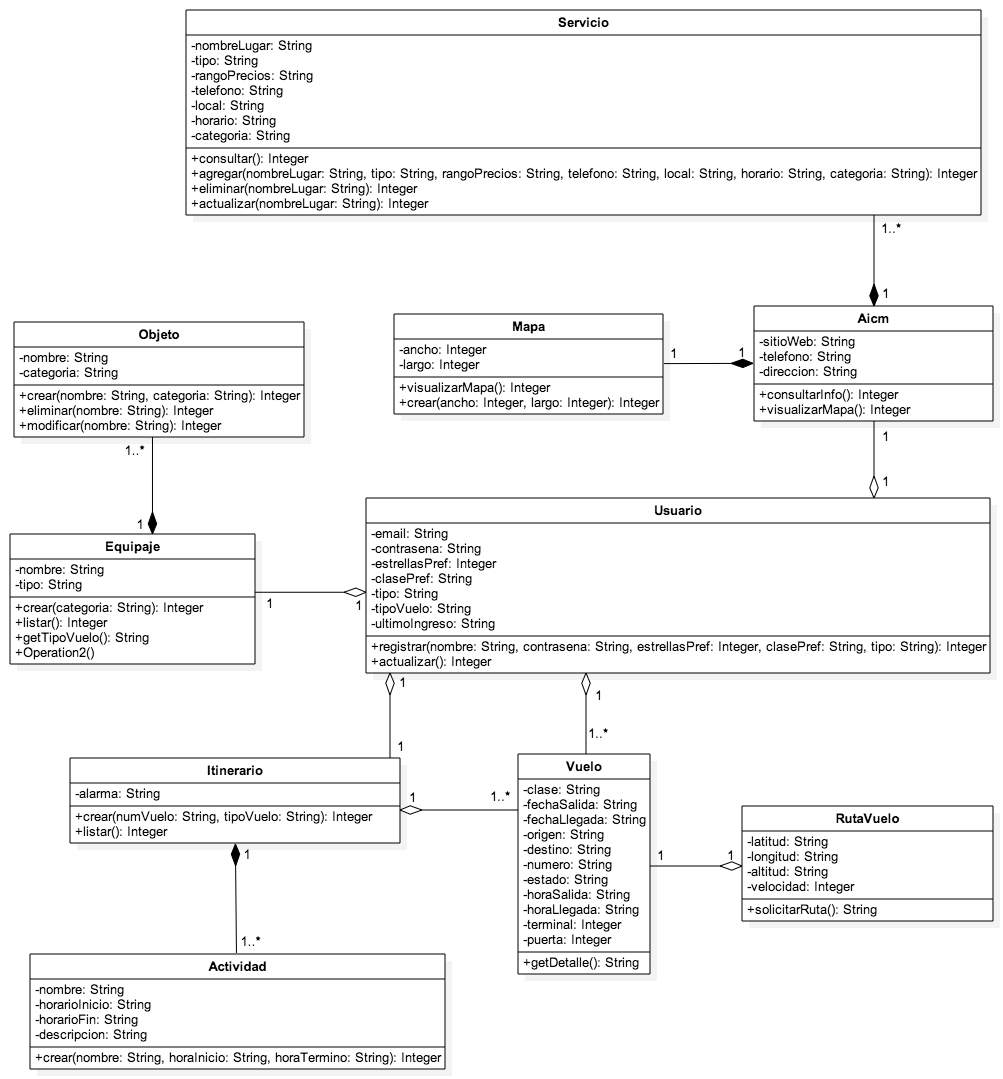
\includegraphics[width=1\textwidth]{Figuras/diagramaClasesMovil.png}
		\rule{30em}{0.5pt}
	\caption[Diagrama de Clases]{Diagrama de Clases}
	\label{fig:diagramaClases}
\end{figure}
\newpage
\section{Diseño de Esquema de Base de Datos}

En las Figuras \ref{fig:relacionalAdmin} y \ref{fig:relacionalMovil} se observa el modelo relacional de las bases de datos del sistema.

\begin{figure}[h!]
	\centering
		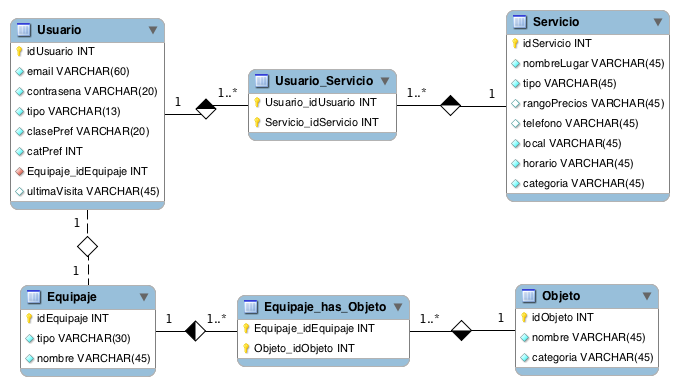
\includegraphics[width=0.8\textwidth]{Figuras/relacionalAdmin.png}
		\rule{30em}{0.5pt}
	\caption[Modelo Relacional de la Aplicación de Escritorio]{Modelo Relacional de la Aplicación de Escritorio}
	\label{fig:relacionalAdmin}
\end{figure}

\begin{figure}[h!]
	\centering
		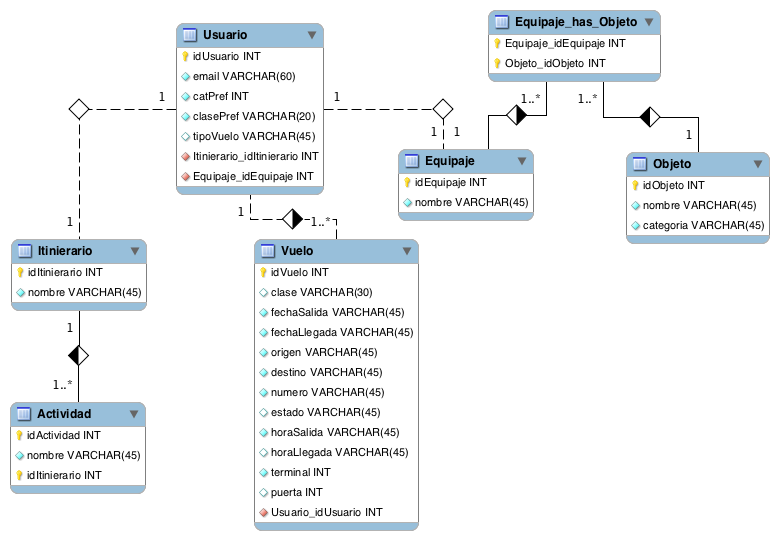
\includegraphics[width=1\textwidth]{Figuras/relacionalMovil.png}
		\rule{30em}{0.5pt}
	\caption[Modelo Relacional de la Aplicación Móvil]{Modelo Relacional de la Aplicación Móvil}
	\label{fig:relacionalMovil}
\end{figure}
\section{Diagramas de Secuencia}

Los diagramas de secuencia es una manera de describir más detalladamente los pasos y procesos a ejecutar para poder cubrir con los puntos de funcionalidad de cada caso de uso. 

\begin{figure}[h]
	\centering
		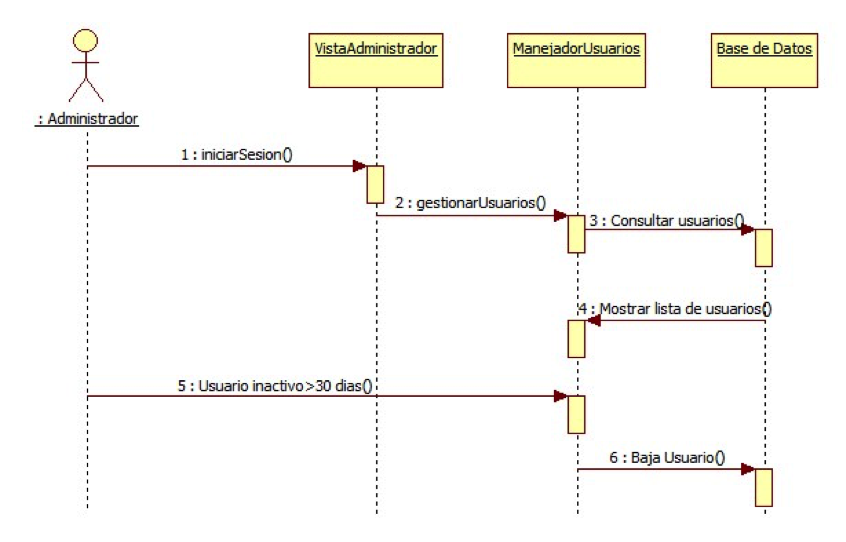
\includegraphics[width=1\textwidth]{Figuras/secGestionarUsuario.png}
		\rule{30em}{0.5pt}
	\caption[Diagrama de Secuencia Gestionar Usuario]{Diagrama de Secuencia Gestionar Usuario}
	\label{fig:secGestionarUsuario}
\end{figure}

\begin{figure}[h]
	\centering
		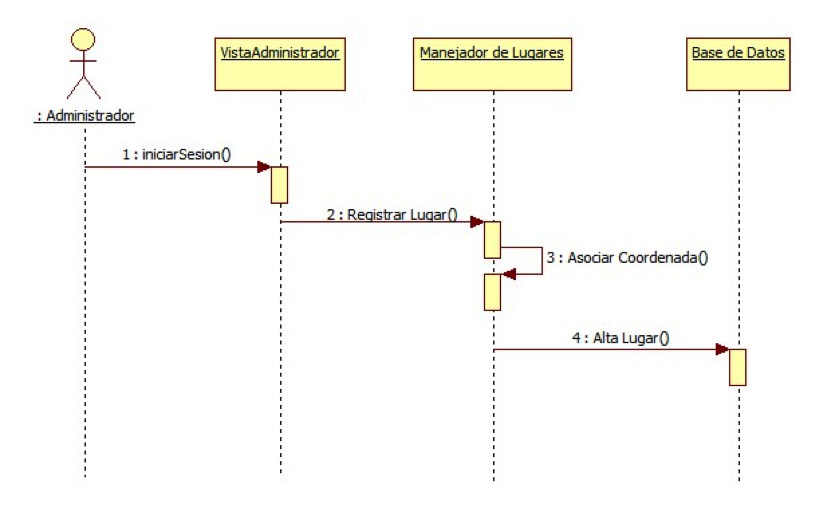
\includegraphics[width=1\textwidth]{Figuras/secRegistrarEquipaje.png}
		\rule{30em}{0.5pt}
	\caption[Diagrama de Secuencia Registrar Equipaje]{Diagrama de Secuencia Registrar Equipaje}
	\label{fig:secRegistrarEquipaje}
\end{figure}

\begin{figure}[h]
	\centering
		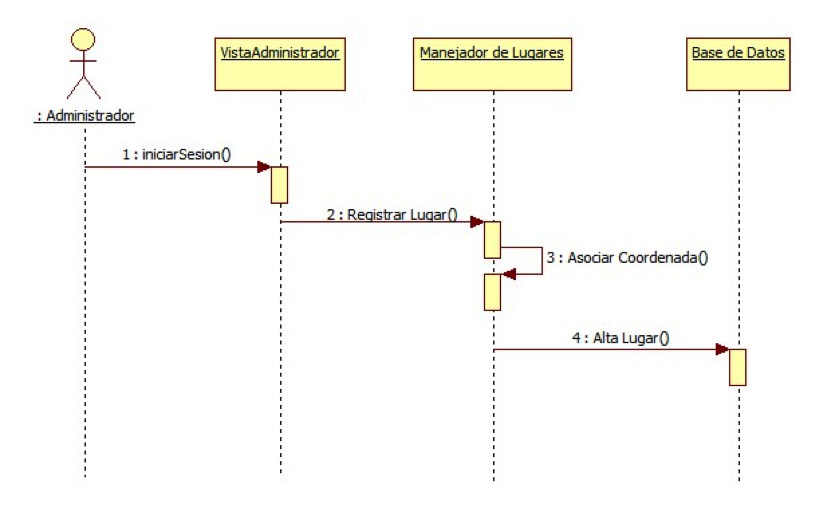
\includegraphics[width=1\textwidth]{Figuras/secGestionarLugar.png}
		\rule{30em}{0.5pt}
	\caption[Diagrama de Secuencia Gestionar Lugar]{Diagrama de Secuencia Gestionar Lugar}
	\label{fig:secGestionarLugar}
\end{figure}

\begin{figure}[h]
	\centering
		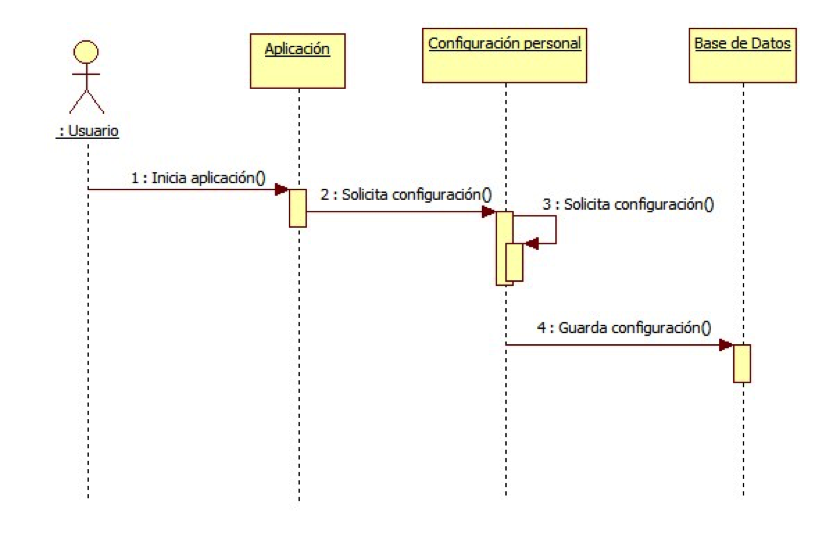
\includegraphics[width=1\textwidth]{Figuras/secConfigurarViaje.png}
		\rule{30em}{0.5pt}
	\caption[Diagrama de Secuencia Configurar Viaje]{Diagrama de Secuencia Configurar Viaje}
	\label{fig:secConfigurarViaje}
\end{figure}

\begin{figure}[h]
	\centering
		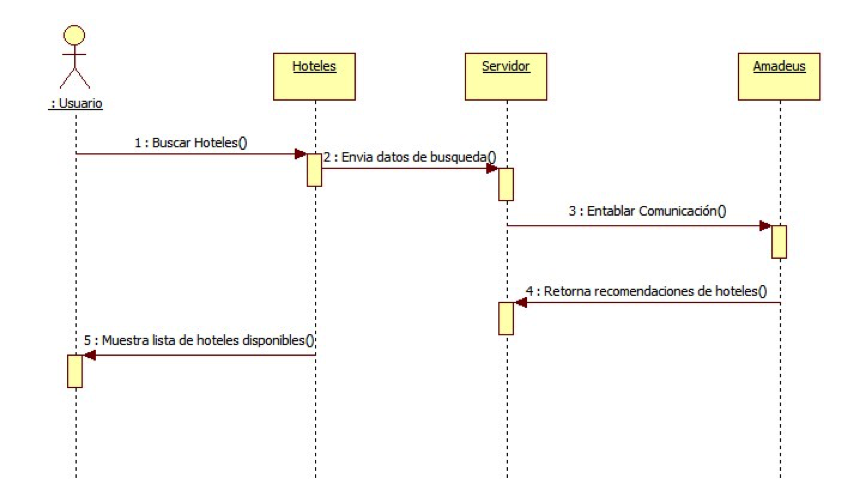
\includegraphics[width=1\textwidth]{Figuras/secConsultarHotel.png}
		\rule{30em}{0.5pt}
	\caption[Diagrama de Secuencia Consultar Hotel]{Diagrama de Secuencia Consultar Hotel}
	\label{fig:secConsultarHotel}
\end{figure}

\begin{figure}[h]
	\centering
		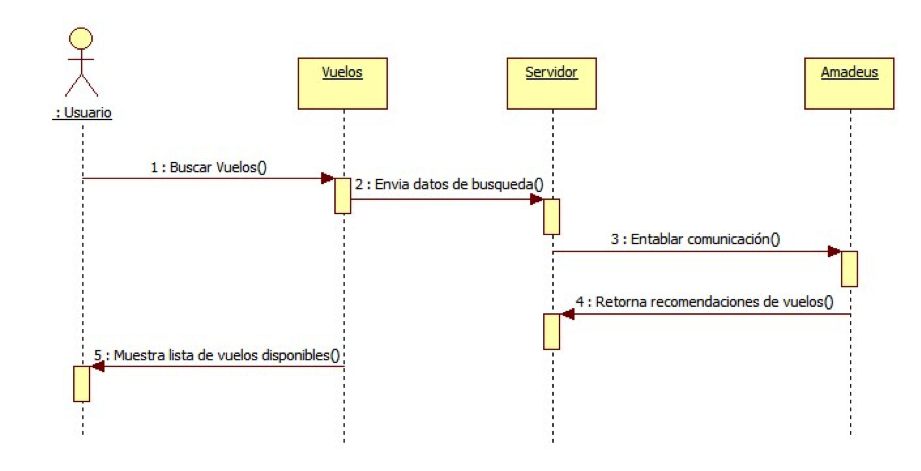
\includegraphics[width=1\textwidth]{Figuras/secConsultarVuelo.png}
		\rule{30em}{0.5pt}
	\caption[Diagrama de Secuencia Consultar Vuelo]{Diagrama de Secuencia Consultar Vuelo}
	\label{fig:secConsultarVuelo}
\end{figure}

\begin{figure}[h]
	\centering
		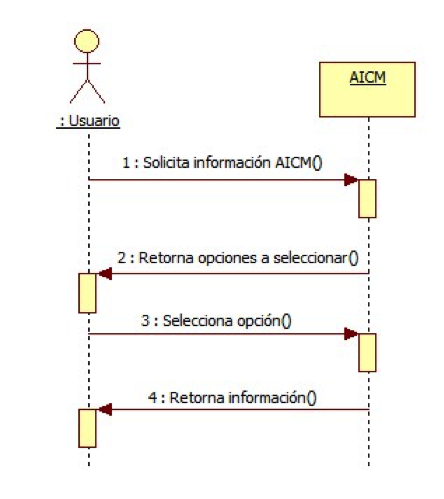
\includegraphics[width=1\textwidth]{Figuras/secConsultarInformacionAICM.png}
		\rule{30em}{0.5pt}
	\caption[Diagrama de Secuencia Consultar Información AICM]{Diagrama de Secuencia Consultar Información AICM}
	\label{fig:secConsultarInformacionAICM}
\end{figure}

\begin{figure}[h]
	\centering
		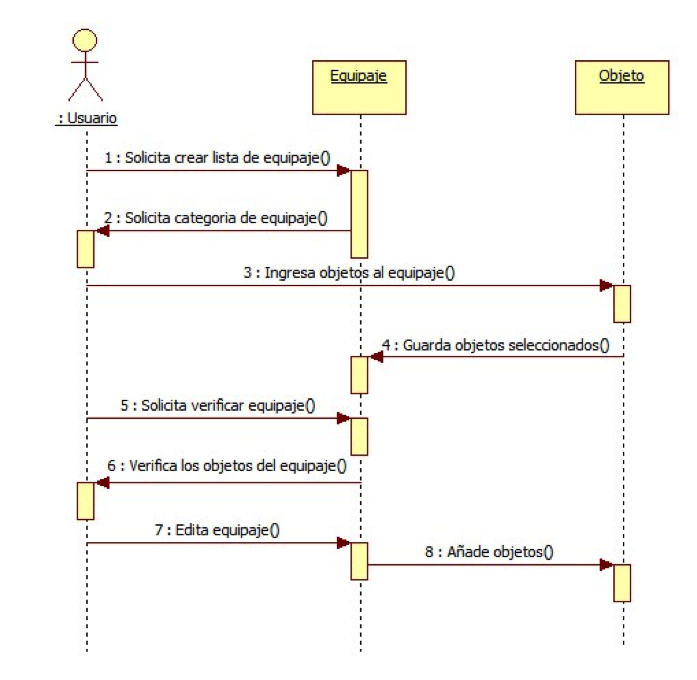
\includegraphics[width=1\textwidth]{Figuras/secGestionarEquipaje.png}
		\rule{30em}{0.5pt}
	\caption[Diagrama de Secuencia Gestionar Equipaje]{Diagrama de Secuencia Gestionar Equipaje}
	\label{fig:secGestionarEquipaje}
\end{figure}

\begin{figure}[h]
	\centering
		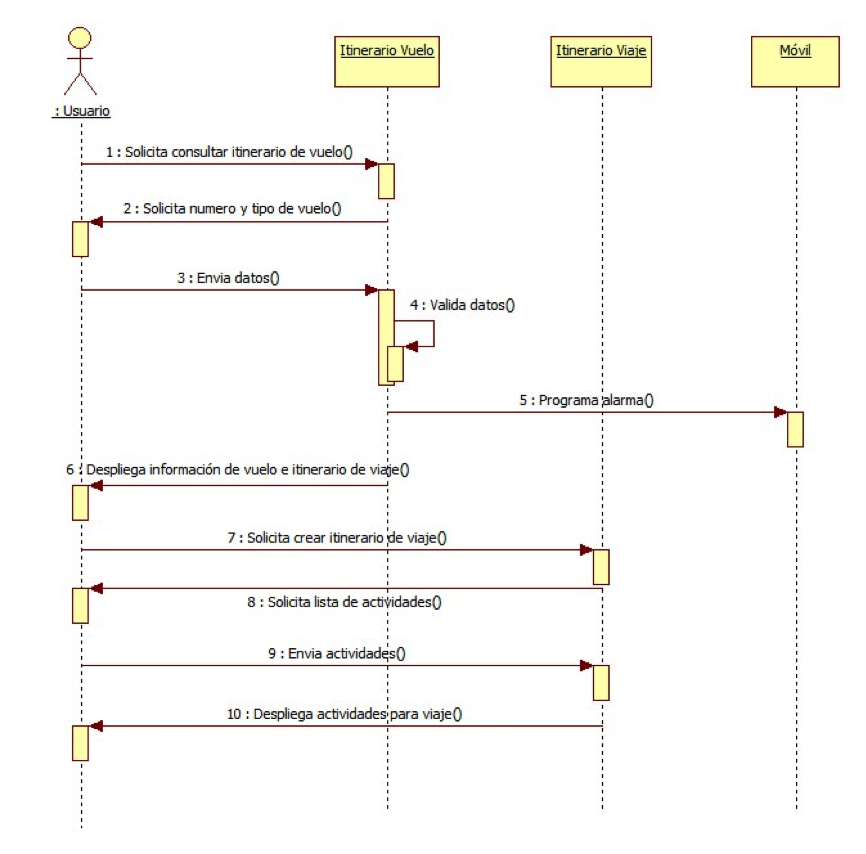
\includegraphics[width=1\textwidth]{Figuras/secConsultarItinerarioViaje.png}
		\rule{30em}{0.5pt}
	\caption[Diagrama de Secuencia Consultar Itinerario de Viaje]{Diagrama de Secuencia Consultar Itinerario de Viaje}
	\label{fig:secConsultarItinerarioViaje}
\end{figure}

\begin{figure}[h]
	\centering
		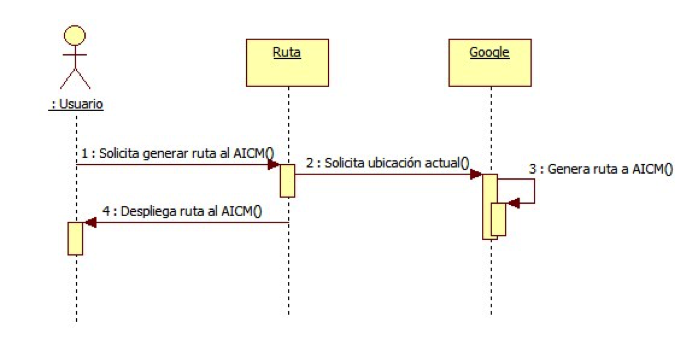
\includegraphics[width=1\textwidth]{Figuras/secConsultarRutacasa-AICM.png}
		\rule{30em}{0.5pt}
	\caption[Diagrama de Secuencia Consultar Ruta casa-AICM]{Diagrama de Secuencia Consultar Ruta casa-AICM}
	\label{fig:secConsultarRutacasa-AICM}
\end{figure}

\begin{figure}[h]
	\centering
		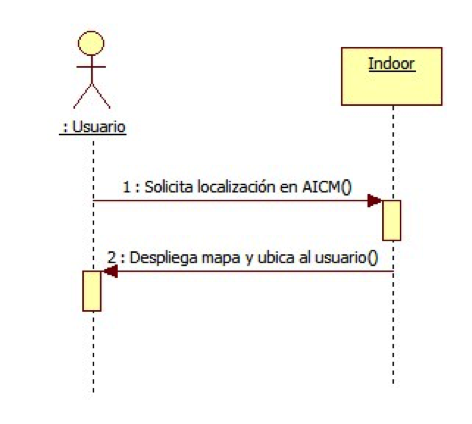
\includegraphics[width=1\textwidth]{Figuras/secUbicarAICM.png}
		\rule{30em}{0.5pt}
	\caption[Diagrama de Secuencia Ubicar en AICM]{Diagrama de Secuencia Ubicar en AICM}
	\label{fig:secUbicarAICM}
\end{figure}

\begin{figure}[h]
	\centering
		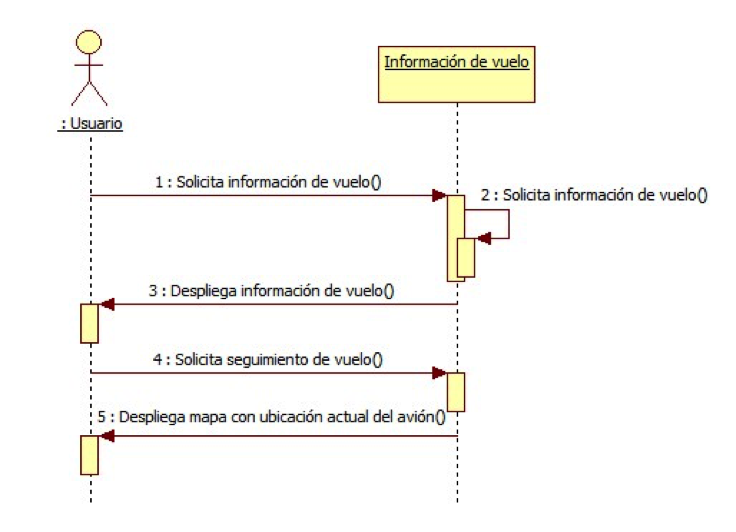
\includegraphics[width=1\textwidth]{Figuras/secConsultarInformacionVuelo.png}
		\rule{30em}{0.5pt}
	\caption[Diagrama de Secuencia Consultar Información de Vuelo]{Diagrama de Secuencia Consultar Información de Vuelo}
	\label{fig:secConsultarInformacionVuelo}
\end{figure}
\clearpage
\section{Diagrama de Despliegue}

A continuación se describe la topología del sistema mediante un diagrama de despliegue, el cual muestra la estructura de los elementos de hardware y el software utilizado por cada uno de estos, así como las relaciones presentes entre los elementos y la forma en que se comunican entre ellos.

\begin{figure}[h]
	\centering
		\includegraphics[width=1\textwidth]{Figuras/diagramaDespliegue.png}
		\rule{30em}{0.5pt}
	\caption[Diagrama de Despliegue]{Diagrama de Despliegue}
	\label{fig:diagramaDespliegue}
\end{figure}

El sistema consta de 8 elementos:

\begin{enumerate}
	\item Dispositivo móvil de Android.
	\item Servidor de peticiones Linux.
	\item Servidor de base de datos MySQL.
	\item Servidor de base de datos SQLite.
	\item Servidor de geolocalización Google.
	\item Servidor de localización en interiores IndoorAtlas.
	\item Servidor de servicios turísticos Amadeus.
	\item Servicio web TASMC.
\end{enumerate}

Estos dispositivos interactúan entre sí de la siguiente manera: 

El dispositivo móvil a través de la Interfaz Grafica de Usuario, manda a llamar mediante consultas SQL el servidor de base de datos de SQLite para obtener instancias de equipaje, itinerario e información del AICM, se envía una petición al Servidor de Geolocalización en formato JSON y llama el Servicio Web de Rutas, además de solicitar al Servidor de servicios turísticos mediante una intercambio SOAP/XML recomendaciones de hoteles y vuelos y finalmente la interacción a través de SOAP con el Servicio Web propio de TASMC que estará conectado con el servidor que se comunica con el Servidor de base de datos MySQL  que recibe peticiones SQL y busca instancias de usuarios, lugares y objetos que van a ser gestionados por el administrador del sistema y donde quedan registrados los lugares que serán representados en la interacción del dispositivo móvil con el servidor de localización en interiores IndoorAtlas.

\clearpage
\section{Diseño de la Interfaz Gráfica del Usuario}

\hypertarget{CU-U-01-1}{}
\subsection{Pantalla CU-U-01-1: Configurar viaje}
\textbf{Objetivo}\\
Personalizar la aplicación TASMC con gustos o preferencias de vuelos y hoteles. \\

\textbf{Diseño:}
\begin{figure}[h]
	\centering
		\includegraphics[width=0.4\textwidth]{Figuras/intConfiguracion.png}
		\rule{30em}{0.5pt}
	\caption[Pantalla configurar viaje]{Pantalla configurar viaje}
	\label{fig:intConfiguracion}
\end{figure}

\textbf{Descripción} \\
Los campos email y contraseña, se utilizan para el registro del usuario. Clase de viaje y categoría de hotel, requieren información que el usuario debe proporcionar para que la personalización de su viaje sea mejor. Finalmente, se obsera un botón que envia los datos del formulario a la aplicación web de TASMC. \\

\textbf{Entradas}
\begin{itemize}
\item Se escribe el email del usuario.
\item Se escribe la contraseña que el usuario utilizará para ingresar a los datos de TASMC.
\item Se escribe la clase en la cual el usuario prefiere al volar.
\item Se escribe la categoría de los hoteles que se prefieren. 
\end{itemize}

\textbf{Salidas}
\begin{itemize}
\item Se envian los datos a la base de datos.
\end{itemize}

\textbf{Controles}
\begin{itemize}
\item Botón Enviar, hará llegar la información al administrador.
\end{itemize}
\clearpage
\hypertarget{CU-U-02-1}{}
\subsection{Pantalla CU-U-02-1: Consultar Hotel}
\textbf{Objetivo}\\
Mostrar información de hoteles. \\

\textbf{Diseño:}
\begin{figure}[h]
	\centering
		\includegraphics[width=0.4\textwidth]{Figuras/intHoteles.jpg}
		\rule{30em}{0.5pt}
	\caption[Pantalla consultar hotel]{Pantalla consultar hotel}
	\label{fig:intHoteles}
\end{figure}

\textbf{Descripción} \\
El campo "Nombre de la ciudad o lugar" es para ingresar la ciudad donde se estará buscando hotel y el botón "Buscar Hoteles" nos permite realizar la búsqueda utilizando como parámetro el nombre de la ciudad. \\

\textbf{Entradas}
\begin{itemize}
\item Se escribe la ciudad donde se alojará el usuario.
\end{itemize}

\textbf{Salidas}
\begin{itemize}
\item Se realiza la búsqueda del hotel.
\end{itemize}

\textbf{Controles}
\begin{itemize}
\item Botón Buscar Hoteles, permite realizar la búsqueda.
\end{itemize}
\clearpage
\hypertarget{CU-U-03-1}{}
\subsection{Pantalla CU-U-03-1: Consultar Vuelo}
\textbf{Objetivo}\\
Mostrar información de vuelos. \\

\textbf{Diseño:}
\begin{figure}[h]
	\centering
		\includegraphics[width=0.4\textwidth]{Figuras/intConsultarVuelo.png}
		\rule{30em}{0.5pt}
	\caption[Pantalla consultar vuelo]{Pantalla consultar vuelo}
	\label{fig:intHoteles}
\end{figure}

\textbf{Descripción} \\
Los "Desde" y "A" son para ingresar la ciudad origen y destino del viaje. El siguiente campo es para ingresar la fecha de salida y, finalmente, se tiene un campo para ingresar la clase de vuelo que se busca. \\

\textbf{Entradas}
\begin{itemize}
\item Se escribe la ciudad origen.
\item Se escribe la ciudad destino.
\item Se ingresa la fecha de salida.
\item Se ingresa la clase de vuelo.
\end{itemize}

\textbf{Salidas}
\begin{itemize}
\item Se realiza la búsqueda del vuelo.
\end{itemize}

\textbf{Controles}
\begin{itemize}
\item Botón Buscar Vuelos, permite realizar la búsqueda.
\end{itemize}
\clearpage
\hypertarget{CU-U-04-1}{}
\subsection{Pantalla CU-U-04-1: Consultar Información AICM}
\textbf{Objetivo}\\
Mostrar información del AICM. \\

\textbf{Diseño:}
\begin{figure}[h]
	\centering
		\includegraphics[width=0.4\textwidth]{Figuras/intConsultarInformacionAICM.png}
		\rule{30em}{0.5pt}
	\caption[Pantalla consultar información AICM]{Pantalla consultar información AICM}
	\label{fig:intConsultarInformacionAICM}
\end{figure}

\textbf{Descripción} \\
Es una pantalla con diferentes pestañas, cada una brinda información sobre el AICM. El teléfono, página web, dirección, mapa interior y Servicios, será la información que se pueda consultar. \\

\textbf{Entradas}
\begin{itemize}
\item Se elige una pestaña.
\end{itemize}

\textbf{Salidas}
\begin{itemize}
\item Se abre la pestaña elegida para visualizar la información que contiene.
\end{itemize}
\clearpage
\hypertarget{CU-U-05-1}{}
\subsection{Pantalla CU-U-05-1: Gestionar Equipaje}
\textbf{Objetivo}\\
Mostrar las listas de equipaje disponibles y las opciones de agregar, editar o eliminar una lista y/o sus objetos. \\

\textbf{Diseño:}
\begin{figure}[h]
	\centering
		\includegraphics[width=0.4\textwidth]{Figuras/intListaEquipaje.jpg}
		\rule{30em}{0.5pt}
	\caption[Pantalla Equipaje]{Pantalla Equipaje}
	\label{fig:intListaEquipaje}
\end{figure}

\textbf{Descripción} \\
Se visualizan 4 listas predefinidas, el usuario puede abrir cualquiera para ver su contenido. También está el icono "+" el cual nos da la opción de crear una nueva lista. \\

\textbf{Entradas}
\begin{itemize}
\item Se elige una lista para visualizar su contenido.
\item Se elige crear una nueva lista.
\end{itemize}

\textbf{Salidas}
\begin{itemize}
\item Muestra un listado de objetos que son el contenido del equipaje elegido.
\end{itemize}

\textbf{Controles}
\begin{itemize}
\item Botón agregar, para ingresar una nueva lista de objetos.
\end{itemize}
\clearpage
\hypertarget{CU-U-06-1}{}
\subsection{Pantalla CU-U-06-1: Consultar Itinerario de Viaje}
\textbf{Objetivo}\\
Mostrar al usuario el itinerario de su viaje. \\

\textbf{Diseño:}
\begin{figure}[h]
	\centering
		\includegraphics[width=0.4\textwidth]{Figuras/intItinerarioViaje.jpg}
		\rule{30em}{0.5pt}
	\caption[Pantalla Itinerario de Viaje]{Pantalla Itinerario de Viaje}
	\label{fig:intItinerarioViaje}
\end{figure}

\textbf{Descripción} \\
Se visualizan 4 botones para ingresar nuevas actividades, para guardar el itinerario, para visualizar el itinerario y para poner como favorita cierta actividad. \\

\textbf{Entradas}
\begin{itemize}
\item Se elige una opción para ejecutar la acción de algún botón.
\end{itemize}

\textbf{Salidas}
\begin{itemize}
\item Muestra la tarea del botón elegido.
\end{itemize}

\textbf{Controles}
\begin{itemize}
\item Botón agregar, para ingresar una nueva actividad
\item Botón guardar, para actualzar el itinerario con las actividades nuevas.
\item Botón ver, para visualizar el itinerario.
\item Botón favorito, para marcar alguna actividad como favorito.
\end{itemize}
\clearpage
\hypertarget{CU-U-07-1}{}
\subsection{Pantalla CU-U-07-1: Consultar Ruta casa-AICM}
\textbf{Objetivo}\\
Mostrar la ruta para llegar al AICM \\

\textbf{Diseño:}
\begin{figure}[h]
	\centering
		\includegraphics[width=0.4\textwidth]{Figuras/intRutaAICM.jpg}
		\rule{30em}{0.5pt}
	\caption[Pantalla Ruta AICM]{Pantalla Ruta AICM}
	\label{fig:intRutaAICM}
\end{figure}

\textbf{Descripción} \\
Se visualiza un mapa con la ruta desde el punto donde se encuentre el usuario hasta el AICM. \\

\textbf{Entradas}
\begin{itemize}
\item Se oprime el botón del menú para ingresar a la presente pantalla.
\end{itemize}

\textbf{Salidas}
\begin{itemize}
\item Muestra la presente pantalla con la ruta al AICM.
\end{itemize}
\clearpage
\hypertarget{CU-U-08-1}{}
\subsection{Pantalla CU-U-08-1: Ubicar en AICM}
\textbf{Objetivo}\\
Apoyar al usuario para ubicarse dento del AICM. \\

\textbf{Diseño:}
\begin{figure}[h]
	\centering
		\includegraphics[width=0.4\textwidth]{Figuras/intUbicarAICM.png}
		\rule{30em}{0.5pt}
	\caption[Pantalla Ubicar en AICM]{Pantalla Ubicar en AICM}
	\label{fig:intUbicarAICM}
\end{figure}

\textbf{Descripción} \\
Se visualiza un mapa con el interior del AICM para que el usuario pueda ubicarse dentro del mismo y, de esa forma, no perderse mientras busca algún lugar de su interés. También podemos observar que se muestran los iconos de servicios en el AICM. \\

\textbf{Entradas}
\begin{itemize}
\item Se ingresa al mapa del AICM
\end{itemize}

\textbf{Salidas}
\begin{itemize}
\item Muestra el AICM y sus servicios según la zona donde se encuentre el usuario.
\end{itemize}
\clearpage
\hypertarget{CU-U-09-1}{}
\subsection{Pantalla CU-U-09-1: Consultar Innformación de Vuelo}
\textbf{Objetivo}\\
Permitir visualizar la información del vuelo en donde el usuario va a ingresar. \\

\textbf{Diseño:}
\begin{figure}[h]
	\centering
		\includegraphics[width=0.4\textwidth]{Figuras/intInformacionVuelo.png}
		\rule{30em}{0.5pt}
	\caption[Pantalla Información del Vuelo]{Pantalla Información del Vuelo}
	\label{fig:intInformacionVuelo}
\end{figure}

\textbf{Descripción} \\
Se visualizan la información del vuelo del usuario. \\

\textbf{Entradas}
\begin{itemize}
\item Se oprime el botón del menú para ingresar a la presente pantalla.
\end{itemize}

\textbf{Salidas}
\begin{itemize}
\item Muestra la presente pantalla con la información del vuelo.
\end{itemize}
% Capitulo 8

\chapter{Desarrollo e Implementación del Sistema} % Main chapter title

\label{DesarrolloTASMC} % For referencing the chapter elsewhere, use \ref{Chapter1} 

\lhead{Capítulo 8 \emph{Desarrollo e implementacion de TASMC}} % This is for the header on each page - perhaps a shortened title

\section{Introducción}
Este capítulo describe la estructura y el funcionamiento del sistema, tanto del lado del servidor como del cliente. Por un lado, tenemos la aplicación móvil (Cliente), la cual consume los servicios ofrecidos por el servidor y por lo tanto se detalla la navegación e interacción para tener acceso tanto a la información como a las funcionalidades que ofrece.
Para el lado del servidor, se detalla la estructura del sistema web utilizado por el administrador para gestionar la información almacenada en el sistema y sus principales funcionalidades, por lo que se muestran también las principales vistas a las que tiene acceso el administrador.

\section{Aplicación Web (Servidor)}

El sistema del Administrador tiene como finalidad el poder gestionar los usuarios,servicios y de listas de equipaje.
Esto permite tener el control sobre los contenidos que el Usuario puede ver desde su aplicación móvil. También, nos da la posibilidad
de extender la información referente a los servicios dentro del AICM-T1 y, en general, mantenerla actualizada sin importar los cambios
que se vayan dando en el AICM-T1.

Por último, es importante mencionar que este módulo incluso nos permite agregar y gestionar sugerencias de listas de equipaje útiles 
para el viajero. Además de mantener un control sobre el número de usuarios de la aplicación.

\subsection{Generalidades}
El sistema de Administración utiliza las siguientes tecnologías para llevar a cabo sus funciones:
\begin{itemize}
 \item 
\end{itemize}

\subsection{Funcionalidades}

\subsubsection{Iniciar Sesión}
El administrador deberá ingresar su correo y contraseña que le fueron asignados para la gestión de los recursos de la aplicación. A partir 
de ello se mostrará una página principal la cual contiene un menú para ingresar a los distintos módulos.

\begin{figure}[h!]
	\centering
		\includegraphics[width=1\textwidth]{Figuras/principalTASMC.png}
		\rule{35em}{0.5pt}
	\caption[Iniciar sesión aplicación web]{Iniciar sesión aplicación web}
	\label{fig:vistaInicio}
\end{figure}
\clearpage

\begin{figure}[h!]
	\centering
		\includegraphics[width=1\textwidth]{Figuras/index.png}
		\rule{35em}{0.5pt}
	\caption[Página principal TASMC]{Página principal TASMC}
	\label{fig:indexWeb}
\end{figure}
\begin{figure}[h!]
	\centering
		\includegraphics[width=1\textwidth]{Figuras/indexhome.png}
		\rule{35em}{0.5pt}
	\caption[Menú Inicio]{Menú Inicio}
	\label{fig:menuInicio}
\end{figure}
\clearpage

\subsubsection{Gestionar Usuario}
Está sección será únicamente de verficación, es decir, para tener un seguimiento y control de los usuarios activos de la aplicación móvil 
mediante un campo de última visita que muestra la hora y fecha en la cual el usuario uso la aplicación por última vez.
\begin{figure}[h!]
	\centering
		\includegraphics[width=1\textwidth]{Figuras/indexUsuario.png}
		\rule{35em}{0.5pt}
	\caption[Menú Usuario]{Menú Usuario}
	\label{fig:menuUsuario}
\end{figure}
\begin{figure}[h!]
	\centering
		\includegraphics[width=1\textwidth]{Figuras/usuarios.png}
		\rule{35em}{0.5pt}
	\caption[Módulo Gestión de Usuarios]{Módulo Gestión de Usuarios}
	\label{fig:moduloUsuarios}
\end{figure}
\clearpage

\subsubsection{Gestionar Equipaje}
En este módulo el admnistrador puede crear nuevas sugerencias de listas de equipaje, cada una con distintos tipos de objetos separados 
por categoría, además de poder crear nuevos objetos asociados a una categoría específica. Las listas de sugerencia de equipaje estarán 
reflejadas dentro de la aplicación móvil pero las listas creadas propias del usuario no se mostrarán en la aplicación web.
\begin{figure}[h!]
	\centering
		\includegraphics[width=1\textwidth]{Figuras/indexEquipaje.png}
		\rule{35em}{0.5pt}
	\caption[Menú Equipaje]{Menú Equipaje}
	\label{fig:menuEquipaje}
\end{figure}
\begin{figure}[h!]
	\centering
		\includegraphics[width=1\textwidth]{Figuras/equipajes.png}
		\rule{35em}{0.5pt}
	\caption[Módulo Gestión de Equipaje]{Módulo Gestión de Equipaje}
	\label{fig:moduloEquipaje}
\end{figure}

\begin{figure}[h!]
	\centering
		\includegraphics[width=1\textwidth]{Figuras/nuevoequipajewb.png}
		\rule{35em}{0.5pt}
	\caption[Función de creación de nuevo equipaje]{Función de creación de nuevo equipaje}
	\label{fig:funcionNuevoEquipaje}
\end{figure}

\begin{figure}[h!]
	\centering
		\includegraphics[width=1\textwidth]{Figuras/objetosEquipaje.png}
		\rule{35em}{0.5pt}
	\caption[Módulo de Gestión de objetos de equipaje]{Módulo de Gestión de objetos de equipaje}
	\label{fig:moduloObjetos}
\end{figure}
\clearpage

\subsubsection{Gestionar Servicio}
En esté módulo se añade la información correspondiente a los distintos servicios con los cuales cuenta el AICM-T1, como es: 
\begin{itemize}
 \item Nombre
 \item Rango de Precios
 \item Local
 \item Categoría
 \item Teléfono
 \item Horario
\end{itemize}

\begin{figure}[h!]
	\centering
		\includegraphics[width=1\textwidth]{Figuras/indexServicio.png}
		\rule{35em}{0.5pt}
	\caption[Menú Servicio]{Menú Servicio}
	\label{fig:menuServicio}
\end{figure}

\begin{figure}[h!]
	\centering
		\includegraphics[width=1\textwidth]{Figuras/servicioswb.png}
		\rule{35em}{0.5pt}
	\caption[Módulo Gestión de Servicios]{Módulo Gestión de Servicios}
	\label{fig:moduloUsuarios}
\end{figure}
\clearpage

\subsubsection{Cerrar Sesión}
El administrador termina su actividad de gestión dentro de la aplicación y cierra sesión.
\begin{figure}[h!]
	\centering
		\includegraphics[width=1\textwidth]{Figuras/indexCerrarSesion.png}
		\rule{35em}{0.5pt}
	\caption[Menú Cerrar Sesión]{Menú Cerrar Sesión}
	\label{fig:menuCerrar}
\end{figure}
\clearpage

\section{Aplicación Móvil (Cliente)}

Una vez que la aplicación es instalada en el dispositivo móvil, es posible comenzar a consumir los servicios ofrecidos por el servidor y hacer uso de las funcionalidades que se tienen disponibles en base a los requerimientos planteados en este documento.
A continuación se muestra la estructura de la aplicación móvil y se detallan las funcionalidades que el usuario tiene a su disposición.

\subsection{Navegación}
La aplicación está compuesta por nueve vistas diferentes, las cuales a su vez, ofrecen diferentes opciones de navegación y configuración que se describirán a detalle. 
Las vistas principales son:
\begin{itemize}
    \item Configuración Personal
    \item Hoteles
    \item Vuelos
    \item Info AICM
    \item Lista de equipaje 
    \item Itinerario de viaje 
    \item Ruta al AICM
    \item Ubícate 
    \item Info vuelo  
    	\end{itemize}

Dichas vistas podrán ser accedidas mediante un menú que se muestra en la vista principal.
\begin{figure}[h]
	\centering
		\includegraphics[width=0.5\textwidth]{Figuras/main.png}
		\rule{30em}{0.5pt}
	\caption[Vista principal de TASMC]{Vista principal de TASMC}
	\label{fig:vistaprincipalTASMC}
\end{figure}

\begin{figure}[h]
	\centering
		\includegraphics[width=0.5\textwidth]{Figuras/menu.png}
		\rule{30em}{0.5pt}
	\caption[Menú de TASMC]{Menú de TASMC}
	\label{fig:menuTASMC}
\end{figure}
\clearpage

\subsection{Módulo Configuración de la aplicación}
Al iniciar la aplicación por primera vez se muestra una vista en la cual el usuario podrá configurar gustos y preferencias según clase en la que prefiere viajar y categoría de hoteles en los que prefiere hospedarse, esto para facilitar la búsqueda de hoteles y vuelos que este desee, 
además de proporcionar su correo electrónico para posibles sugerencias que el sistema le pueda hacer llegar.
En caso de no realizar su configuración podrá solicitar hacerla más tarde dentro de la vista principal de la aplicación.
\begin{figure}[h]
	\centering
		\includegraphics[width=0.5\textwidth]{Figuras/configuracion.png}
		\rule{30em}{0.5pt}
	\caption[Configuración inicial de TASMC]{Configuración inicial de TASMC}
	\label{fig:configuracionTASMC}
\end{figure}
\clearpage

\subsection{Módulo Hoteles}
Al ingresar al módulo de hoteles se mostrara una vista que contiene un formulario el cual servirá para realizar una búsqueda de hoteles, según los parámetros ingresados como son:

\begin{itemize}
\item Nombre de la ciudad o lugar destino.
\item Número de huéspedes.
\item Número de estrellas del hotel.
\end{itemize}

\begin{figure}[h]
	\centering
		\includegraphics[width=0.5\textwidth]{Figuras/hoteles.jpg}
		\rule{30em}{0.5pt}
	\caption[Buscar Hoteles Disponibles]{Buscar Hoteles Disponibles}
	\label{fig:buscarHoteles}
\end{figure}
\clearpage

\subsubsection{Módulo Hoteles Disponibles}
Al realizar la búsqueda de hotel en la vista de Hoteles se mostrará la información 
referente dependiendo de las características que se hayan ingresado y la disponibilidad que exista, como es:
\begin{itemize}
\item Nombre del hotel.
\item Teléfono.
\item Número de estrellas representado por medio de una imagen.
\end{itemize}
\begin{figure}[h]
	\centering
		\includegraphics[width=0.5\textwidth]{Figuras/hdisponible.png}
		\rule{30em}{0.5pt}
	\caption[Hoteles Disponibles]{Hoteles Disponibles}
	\label{fig:hotelesDisponibles}
\end{figure}

\clearpage

\subsubsection{Módulo Detalle Hotel}
Finalmente se podrá obtener la información completa del hotel seleccionado en la lista de hoteles disponibles. Además se mostrará un 
listado de las distintas habitaciones que ofrece el hotel así como teléfono y página web.

\begin{figure}[h]
	\centering
		\includegraphics[width=0.5\textwidth]{Figuras/detalle.png}
		\rule{30em}{0.5pt}
	\caption[Hoteles Disponibles]{Hoteles Disponibles}
	\label{fig:hotelesDisponibles}
\end{figure}

\clearpage

\subsection{Módulo Vuelos}
Este módulo de vuelos mostrará una vista que contiene un formulario el cual servirá para realizar una búsqueda de vuelos, según los parámetros ingresados como son:

\begin{itemize}
\item Origen.
\item Destino.
\item Fecha de Ida.
\item Clase de vuelo.
\end{itemize}

\begin{figure}[h]
	\centering
		\includegraphics[width=0.5\textwidth]{Figuras/buscav.png}
		\rule{30em}{0.5pt}
	\caption[Buscar Vuelos]{Buscar Vuelos}
	\label{fig:vuelos}
\end{figure}
\clearpage

\subsubsection{Módulo Vuelos Disponibles}
Al realizar la búsqueda de vuelo en la vista de Vuelos se mostrará la información referente dependiendo de las características que se hayan ingresado y la disponibilidad que exista, 
como es:
\begin{itemize}
\item Número de vuelo.
\item Hora de salida y llegada.
\item Origen y destino.
\item Aerolínea.
\end{itemize}

\begin{figure}[h]
	\centering
		\includegraphics[width=0.5\textwidth]{Figuras/vdisponibles.png}
		\rule{30em}{0.5pt}
	\caption[Vuelos Disponibles]{Vuelos Disponibles}
	\label{fig:vuelosDisponibles}
\end{figure}
\clearpage

\subsection{Módulo Información del AICM}
A través de esta vista, el sistema muestra la información referente al AICM tales como sitio web, teléfono, ubicación, mapa y servicios.

\begin{figure}[h]
	\centering
		\includegraphics[width=0.5\textwidth]{Figuras/infoaicm.png}
		\rule{30em}{0.5pt}
	\caption[Información del AICM]{Información del AICM}
	\label{fig:infoAICM}
\end{figure}
\clearpage

\subsubsection{Módulo Mapa del AICM}
Al seleccionar el mapa en el módulo de Información del AICM se mostrar una vista la cual se encuentra divida en dos mapas como es la Planta baja y Planta alta del AICM T1.

\begin{figure}[h]
	\centering
		\includegraphics[width=0.5\textwidth]{Figuras/mapapa.png}
		\rule{30em}{0.5pt}
	\caption[Mapa Planta Alta Terminal 1]{Mapa Planta Alta Terminal 1}
	\label{fig:mapaPA}
\end{figure}

\begin{figure}[h]
	\centering
		\includegraphics[width=0.5\textwidth]{Figuras/mapapb.png}
		\rule{30em}{0.5pt}
	\caption[Mapa Planta Baja Terminal 1]{Mapa Planta Baja Terminal 1}
	\label{fig:mapaPB}
\end{figure}
\clearpage

\subsubsection{Módulo Servicios del AICM}
Al seleccionar los servicios en el módulo de Información del AICM se mostrar una lista de los servicios que ofrece el AICM T1.

\begin{figure}[h]
	\centering
		\includegraphics[width=0.5\textwidth]{Figuras/servicios.png}
		\rule{30em}{0.5pt}
	\caption[Servicios Terminal 1]{Servicios Terminal 1}
	\label{fig:servicios}
\end{figure}
\clearpage

\subsection{Módulo Lista de Equipaje}
Este apartado nos muestra una lista con sugerencias de equipajes con un propósito específico así como la opción de generar nuevas listas propias del viajero. 
Dichas sugerencias de equipaje son cargadas directamente de la aplicación web de administración.

\begin{figure}[h]
	\centering
		\includegraphics[width=0.5\textwidth]{Figuras/equipaje.png}
		\rule{30em}{0.5pt}
	\caption[Listas de Equipaje]{Listas de Equipaje}
	\label{fig:equipaje}
\end{figure}
\clearpage

\subsubsection{Módulo Nuevo Equipaje}
Esta vista se muestra cuando se selecciona crear un nuevo equipaje en el modulo de Lista de Equipaje, 
aquí se solicita un nombre y la selección de diversos objetos que el usuario requiera para su viaje.

\begin{figure}[h]
	\centering
		\includegraphics[width=0.5\textwidth]{Figuras/nuevoequipaje.jpg}
		\rule{30em}{0.5pt}
	\caption[Nuevo Equipaje]{Nuevo Equipaje}
	\label{fig:nuevoEquipaje}
\end{figure}
\clearpage

\subsection{Módulo Itinerario de viaje}
Esta vista muestra una lista de itinerarios de viaje que el usuario haya creado, 
mostrando el destino de viaje así como las actividades a realizar en dicho lugar.

\begin{figure}[h]
	\centering
		\includegraphics[width=0.5\textwidth]{Figuras/itinerario.jpg}
		\rule{30em}{0.5pt}
	\caption[Itinerario de viaje]{Itinerario de Viaje}
	\label{fig:itinerario}
\end{figure}
\clearpage

\subsubsection{Módulo Nuevo Itinerario de viaje}
Una vez que se haya solicitado crear un nuevo itinerario de viaje se mostrara una vista donde se podrán ingresar un destino así como las actividades que desee realizar en su viaje.

\begin{figure}[h]
	\centering
		\includegraphics[width=0.5\textwidth]{Figuras/nuevoiti.png}
		\rule{30em}{0.5pt}
	\caption[Nuevo Itinerario de viaje]{Nuevo Itinerario de Viaje}
	\label{fig:nuevoItinerario}
\end{figure}
\clearpage

\subsection{Módulo Ruta al AICM}
Es la vista que muestra un mapa en la cual se encuentran marcados 3 ubicaciones, como es la ubicación principal del AICM y 
las dos terminales con las que cuenta (T1 y T2) esto con el propósito de ofrecerle al usuario la generación de una ruta desde 
su origen el cual puede ser accedido mediante un botón y en el cual resaltara mediante un marcador táctil dicho origen, 
un botón que llevara a la localización principal del AICM y donde de igual manera el usuario seleccionara mediante otro marcador
la terminal requerida, finalmente se podrá visualizar la ruta hacia el AICM.

\begin{figure}[h]
	\centering
		\includegraphics[width=0.5\textwidth]{Figuras/locaicm.png}
		\rule{30em}{0.5pt}
	\caption[Localización AICM]{Localización AICM}
	\label{fig:localizacionAICM}
\end{figure}

\begin{figure}[h]
	\centering
		\includegraphics[width=0.5\textwidth]{Figuras/loct1.png}
		\rule{30em}{0.5pt}
	\caption[Localización Terminal 1]{Localización Terminal 1}
	\label{fig:localizacionT1}
\end{figure}

\begin{figure}[h]
	\centering
		\includegraphics[width=0.5\textwidth]{Figuras/loct2.png}
		\rule{30em}{0.5pt}
	\caption[Localización Terminal 2]{Localización Terminal 2}
	\label{fig:localizacionT2}
\end{figure}

\begin{figure}[h]
	\centering
		\includegraphics[width=0.5\textwidth]{Figuras/locmia.png}
		\rule{30em}{0.5pt}
	\caption[Ubicación Actual]{Ubicación Actual}
	\label{fig:miUbicacion}
\end{figure}

\begin{figure}[h]
	\centering
		\includegraphics[width=0.5\textwidth]{Figuras/ruta.png}
		\rule{30em}{0.5pt}
	\caption[Ruta al AICM]{Ruta al AICM}
	\label{fig:rutaAICM}
\end{figure}
\clearpage

\subsection{Módulo Localización dentro del AICM Terminal 1}
Dicho apartado contendrá el mapa del interior del AICM como es planta alta y baja de la edificación esto con el propósito de brindar un servicio de localización en interiores, 
el cual le permitirá al usuario localizar su sala de abordaje de una manera más rápida.

\begin{figure}[h]
	\centering
		\includegraphics[width=0.5\textwidth]{Figuras/ubikpa.jpg}
		\rule{30em}{0.5pt}
	\caption[Localización en Planta Alta Terminal 1]{Localización en Planta Alta Terminal 1}
	\label{fig:indoorPA}
\end{figure}

\begin{figure}[h]
	\centering
		\includegraphics[width=0.5\textwidth]{Figuras/ubikpb.jpg}
		\rule{30em}{0.5pt}
	\caption[Localización en Planta Baja Terminal 1]{Localización en Planta Baja Terminal 1}
	\label{fig:indoorPB}
\end{figure}
\clearpage

\subsection{Módulo Información de vuelo}
Esta vista permitirá al usuario consultar la información de salidas y llegadas tanto nacionales como internacionales, 
además de buscar mediante su número de vuelo información referente a su vuelo.

\begin{figure}[h]
	\centering
		\includegraphics[width=0.5\textwidth]{Figuras/llegadas.png}
		\rule{30em}{0.5pt}
	\caption[Información de Llegadas Nacionales e Internacionales]{Información de Llegadas Nacionales e Internacionales}
	\label{fig:infoLlegadas}
\end{figure}

\begin{figure}[h]
	\centering
		\includegraphics[width=0.5\textwidth]{Figuras/salidas.png}
		\rule{30em}{0.5pt}
	\caption[Información de Salidas Nacionales e Internacionales]{Información de Salidas Nacionales e Internacionales}
	\label{fig:infoSalidas}
\end{figure}
\clearpage

\subsubsection{Módulo Información de mi vuelo}
Esta vista mostrará información referente al número de vuelo que ingresado en el módulo de Información de vuelo.

\begin{figure}[h]
	\centering
		\includegraphics[width=0.5\textwidth]{Figuras/mivuelo.png}
		\rule{30em}{0.5pt}
	\caption[Información de vuelo]{Información de vuelo}
	\label{fig:infoVuelo}
\end{figure}
\clearpage



\section{Navegación y Gestos}
Como ya se explicó anteriormente la aplicación móvil consta de ocho vistas principales, para poder visualizar cada una de estas, 
es necesario abrir el menú principal de la aplicación deslizando el dedo de izquierda a derecha o presionando el botón en la 
esquina superior izquierda. Para lograr esto se ha utilizado el patrón de diseño conocido como Navigation Drawer y haciendo uso
del componente ActionBar para obtener una fácil navegación asi como utilizar los patrones del material de diseño de Google para 
ofrecer un diseño agradable al usuario.

La Navegación dentro de la aplicación móvil esta basada en cinco gestos sobre la pantalla del dispositivo móvil, a continuación 
se describe cada uno de estos y se menciona en que vistas se utilizan y cuales son las operaciones que nos permiten realizar.

\subsection{Clic Simple}
Este gesto es el más simple y utilizado dentro de la aplicación, consiste únicamente en seleccionar la opción a la que se desea 
acceder mediante un clic simple sobre dicha opción o botón. Posterior a esto se realizara la opción correspondiente a la opción 
seleccionada. Dentro de la aplicación, este gesto es utilizado en: 

\begin{itemize}
 \item Acceso a los distintos módulos dentro del menú principal de TASMC.
 \item Selección de los distintos valores en los formularios de búsqueda de Hoteles y Vuelos, así como el envío de datos por medio 
 de su respectivo botón de búsqueda.
 \item Clic sobre el botón de acción para hacer llamado a una nueva actividad como es la generación de un nuevo itinerario o equipaje.
 \item Clic sobre botones para mostrar la información referente a mapa y servicios dentro del AICM.
 \item Acceso a la edición de listas de equipaje e itinerarios de viaje.
 \item Puntualizar origen y destino mediante marcadores para generar la ruta al AICM.
\end{itemize}

\subsection{Desplazar}
Este gesto consiste en desplazarse por la pantalla de arriba hacia abajo y viceversa. 
Dejando pulsada la pantalla movemos el dedo arriba o abajo. Este gesto es utilizado principalmente en las vistas que contienen 
listas como son:

\begin{itemize}
 \item La lista del menú principal.
 \item Lista de Hoteles Disponibles.
 \item Lista de Equipaje y objetos.
 \item Lista de Itinerarios de Viaje.
 \item Lista de Llegadas y Salidas Nacionales e Internacionales.
\end{itemize}

\subsection{Deslizar}
Este gesto consiste en mantener oprimida la pantalla del dispositivo y deslizar el dedo a lo ancho de la pantalla para intercambiar 
la vista que se esté presentando. Su uso primordial es:

\begin{itemize}
 \item Intercambiar las vistas para la búsqueda de vuelos; ida y redondo.
 \item Intercambio de mapas de Planta Alta y Planta Baja.
 \item Navegación entre las vistas de Salidas y Llegadas.
 \item Deslizar el menú principal.
\end{itemize}

\subsection{Pellizcar}
Es la típica acción que hacemos juntando o separando dos dedos para, por ejemplo, hacer zoom en una imagen. Este gesto es utilizado en:
\begin{itemize}
 \item El zoom de mapas del AICM.
 \item El zoom del mapa de la ruta hacia el AICM.
\end{itemize}

\subsection{Arrastrar}
Por último, este gesto consiste en mantener oprimida el área de selección y deslizar el dedo hacia arriba o hacia un lado para tener 
acceso a la información o funcionalidades correspondientes. 
\begin{itemize}
 \item Es aplicado en la lista de itinerarios, dejando presionado un itinerario y desplazandoló hacia la derecha es posible editar el mismo, 
 desplazandoló hacia la izquierda el itinerario es eliminado de la base de datos.
\end{itemize}

% Capitulo 9

\chapter{Pruebas} % Main chapter title

\label{PruebasTASMC} % For referencing the chapter elsewhere, use \ref{Chapter1} 

\lhead{Capítulo 9 \emph{Pruebas}} % This is for the header on each page - perhaps a shortened title

\section{Pruebas de Casos de Uso principales}
La aplicación móvil se compone de nueve vistas principales:
\begin{itemize}
 \item Configuración Personal
 \item Hoteles
 \item Vuelos
 \item Info AICM
 \item Lista de Equipaje
 \item Itinerario de viaje
 \item Ruta al AICM
 \item Ubícate
 \item Info Vuelo
\end{itemize}

A su vez cada módulo puede desplegar información diversa en otras vistas o en su caso a partir opciones adicionales sobre un menú 
secundario.
\clearpage

\subsection{Configuración Personal}

\definecolor{blanco}{RGB}{255,255,255}

\begin{table}[h]
	\begin{center}
		\begin{tabular}{|>{\color{blanco}}c|>{\color{blanco}}c|>{\color{blanco}}c|>{\color{blanco}}c|}
			\hline \rowcolor[RGB]{51,153,255} 
				{\bf CU} & 
				{\bf Acción o evento} &
				{\bf Resultados y/u observaciones} &
				{\bf } \\
			\hline 
				\multicolumn{1}{|m{1.8cm}|}{\centering CU-U-01} &
				\multicolumn{1}{m{4.5cm}|}{\centering Clic normal en crear configuración} &
				\multicolumn{1}{m{5.5cm}|}{\centering Se ingresan datos como email, clase de
				viaje y categoría de hotel por número de estrellas.El registro en el web service es exitoso.} &
				\multicolumn{1}{m{1.5cm}|}{\centering \includegraphics[width=8mm, height=8mm]{Figuras/palomita.png}} \\
      		\hline \rowcolor[RGB]{240,248,255} 
				\multicolumn{1}{|m{1.8cm}|}{\centering CU-U-01} &
				\multicolumn{1}{m{4.5cm}|}{\centering Clic normal en evitar configuración} &
				\multicolumn{1}{m{5.5cm}|}{\centering Se muestra el menú principal de TASMC y la opción de configurar sobre un 
				menú secundario.} &
				\multicolumn{1}{m{1.5cm}|}{\centering \includegraphics[width=8mm, height=8mm]{Figuras/palomita.png}} \\
		\hline 
				\multicolumn{1}{|m{1.8cm}|}{\centering CU-U-01} &
				\multicolumn{1}{m{4.4cm}|}{\centering Clic normal en opción de reconfiguración} &
				\multicolumn{1}{m{5.5cm}|}{\centering Se ingresan los datos de email, clase de viaje y categoría de 
				hotel. La fecha de configuración del usuario es modificada dentro del web service de administración.} &
				\multicolumn{1}{m{1.5cm}|}{\centering \includegraphics[width=8mm, height=8mm]{Figuras/palomita.png}} \\
      		\hline 
		\end{tabular}
	\end{center}
	\caption[Pruebas del módulo de Configuración Personal]{Pruebas del módulo de Configuración Personal} 
	\label{tab:pruebasConfiguracion}
\end{table}

\subsection{Hoteles}

\definecolor{blanco}{RGB}{255,255,255}

\begin{table}[h]
	\begin{center}
		\begin{tabular}{|>{\color{blanco}}c|>{\color{blanco}}c|>{\color{blanco}}c|>{\color{blanco}}c|}
			\hline \rowcolor[RGB]{51,153,255} 
				{\bf CU} & 
				{\bf Acción o evento} &
				{\bf Resultados y/u observaciones} &
				{\bf } \\
			\hline 
				\multicolumn{1}{|m{1.8cm}|}{\centering CU-U-02} &
				\multicolumn{1}{m{4.5cm}|}{\centering Clic normal en búsqueda de hoteles} &
				\multicolumn{1}{m{5.5cm}|}{\centering Despliega la información de hoteles correspondiente a las parámetros ingresados 
				en el formulario.} &
				\multicolumn{1}{m{1.5cm}|}{\centering \includegraphics[width=8mm, height=8mm]{Figuras/palomita.png}} \\
      		\hline \rowcolor[RGB]{240,248,255} 
				\multicolumn{1}{|m{1.8cm}|}{\centering CU-U-02} &
				\multicolumn{1}{m{4.5cm}|}{\centering Clic normal en detalle de hotel} &
				\multicolumn{1}{m{5.5cm}|}{\centering Muestra la información completa del hotel.} &
				\multicolumn{1}{m{1.5cm}|}{\centering \includegraphics[width=8mm, height=8mm]{Figuras/palomita.png}} \\
		\hline 
				\multicolumn{1}{|m{1.8cm}|}{\centering CU-U-02} &
				\multicolumn{1}{m{4.5cm}|}{\centering Clic normal en llamar hotel} &
				\multicolumn{1}{m{5.5cm}|}{\centering Activa el servicio de llamada hacia el número propio del hotel.} &
				\multicolumn{1}{m{1.5cm}|}{\centering \includegraphics[width=8mm, height=8mm]{Figuras/palomita.png}} \\
      		\hline \rowcolor[RGB]{240,248,255} 
				\multicolumn{1}{|m{1.8cm}|}{\centering CU-U-02} &
				\multicolumn{1}{m{4.5cm}|}{\centering Clic normal en página web del hotel} &
				\multicolumn{1}{m{5.5cm}|}{\centering Abre la página web propia del hotel en el navegador del teléfono.} &
				\multicolumn{1}{m{1.5cm}|}{\centering \includegraphics[width=8mm, height=8mm]{Figuras/palomita.png}} \\
      		        \hline 
      		        
		\end{tabular}
	\end{center}
	\caption[Pruebas del módulo de Hoteles]{Pruebas del módulo de Hoteles} 
	\label{tab:pruebasHoteles}
\end{table}
\clearpage

\subsection{Vuelos}

\definecolor{blanco}{RGB}{255,255,255}

\begin{table}[h]
	\begin{center}
		\begin{tabular}{|>{\color{blanco}}c|>{\color{blanco}}c|>{\color{blanco}}c|>{\color{blanco}}c|}
			\hline \rowcolor[RGB]{51,153,255} 
				{\bf CU} & 
				{\bf Acción o evento} &
				{\bf Resultados y/u observaciones} &
				{\bf } \\
			\hline 
				\multicolumn{1}{|m{1.8cm}|}{\centering CU-U-03} &
				\multicolumn{1}{m{4.5cm}|}{\centering Clic normal en búsqueda de vuelos} &
				\multicolumn{1}{m{5.5cm}|}{\centering Despliega la información correspondiente de vuelos según los parámetros ingresados 
				en el formulario.} &
				\multicolumn{1}{m{1.5cm}|}{\centering \includegraphics[width=8mm, height=8mm]{Figuras/palomita.png}} \\
			  \hline 
      		\end{tabular}
	\end{center}
	\caption[Pruebas del módulo de Vuelos]{Pruebas del módulo de Vuelos} 
	\label{tab:pruebasVuelos}
\end{table}

\subsection{Info AICM}

\definecolor{blanco}{RGB}{255,255,255}

\begin{table}[h]
	\begin{center}
		\begin{tabular}{|>{\color{blanco}}c|>{\color{blanco}}c|>{\color{blanco}}c|>{\color{blanco}}c|}
			\hline \rowcolor[RGB]{51,153,255} 
				{\bf CU} & 
				{\bf Acción o evento} &
				{\bf Resultados y/u observaciones} &
				{\bf } \\
			\hline 
				\multicolumn{1}{|m{1.8cm}|}{\centering CU-U-04} &
				\multicolumn{1}{m{4.5cm}|}{\centering Clic normal en Info AICM} &
				\multicolumn{1}{m{5.5cm}|}{\centering Despliega la información del AICM como sitio web, teléfono, ubicación, y dos botones para 
				el mapa y los servicios.} &
				\multicolumn{1}{m{1.5cm}|}{\centering \includegraphics[width=8mm, height=8mm]{Figuras/palomita.png}} \\
      		\hline \rowcolor[RGB]{240,248,255} 
      				\multicolumn{1}{|m{1.8cm}|}{\centering CU-U-04} &
				\multicolumn{1}{m{4.5cm}|}{\centering Clic normal en mapa de AICM} &
				\multicolumn{1}{m{5.5cm}|}{\centering Se muestra una vista dividida en planta baja y alta, la cuál 
				puede ser intercambiada mediante un deslizamiento en la pantalla de izquierda a derecha.} &
				\multicolumn{1}{m{1.5cm}|}{\centering \includegraphics[width=8mm, height=8mm]{Figuras/palomita.png}} \\
		\hline 
				\multicolumn{1}{|m{1.8cm}|}{\centering CU-U-04} &
				\multicolumn{1}{m{4.5cm}|}{\centering Clic normal en servicios del AICM} &
				\multicolumn{1}{m{5.5cm}|}{\centering Se una lista de los servicios que ofrece el AICM-T1.} &
				\multicolumn{1}{m{1.5cm}|}{\centering \includegraphics[width=8mm, height=8mm]{Figuras/palomita.png}} \\
      		        \hline 
    		\end{tabular}
	\end{center}
	\caption[Pruebas del módulo de Info AICM]{Pruebas del módulo de Info AICM} 
	\label{tab:pruebasInfoAICM}
\end{table}

\clearpage

\subsection{Lista de Equipaje}

\definecolor{blanco}{RGB}{255,255,255}

\begin{table}[h]
	\begin{center}
		\begin{tabular}{|>{\color{blanco}}c|>{\color{blanco}}c|>{\color{blanco}}c|>{\color{blanco}}c|}
			\hline \rowcolor[RGB]{51,153,255} 
				{\bf CU} & 
				{\bf Acción o evento} &
				{\bf Resultados y/u observaciones} &
				{\bf } \\
			\hline 
				\multicolumn{1}{|m{1.8cm}|}{\centering CU-U-05} &
				\multicolumn{1}{m{4.5cm}|}{\centering Clic normal en Lista de Equipaje} &
				\multicolumn{1}{m{5.5cm}|}{\centering Se despliega una lista de equipajes los cuales pueden ser sugerencias 
				cargadas directamente desde el web service o listas creadas por el usuario. Se muestra un mensaje solicitando al usuario 
				conectarse a internet en caso de no tener encendido ese servicio. No carga las sugerencias de equipajes 
				si no se encuentra conectado a internet.} &
				\multicolumn{1}{m{1.5cm}|}{\centering \includegraphics[width=8mm, height=8mm]{Figuras/palomita.png}} \\
      		\hline \rowcolor[RGB]{240,248,255} 
      				\multicolumn{1}{|m{1.8cm}|}{\centering CU-U-05} &
				\multicolumn{1}{m{4.5cm}|}{\centering Clic normal en botón de nuevo equipaje} &
				\multicolumn{1}{m{5.5cm}|}{\centering Se muestra un vista donde se debe ingresar un nombre para la lista de 
				equipaje asi como una lista con los objetos que desee llevar en su viaje.} &
				\multicolumn{1}{m{1.5cm}|}{\centering \includegraphics[width=8mm, height=8mm]{Figuras/palomita.png}} \\
		\hline 
				\multicolumn{1}{|m{1.8cm}|}{\centering CU-U-05} &
				\multicolumn{1}{m{4.5cm}|}{\centering Clic normal en lista de equipaje} &
				\multicolumn{1}{m{5.5cm}|}{\centering Se muestran una lista con los objetos en el equipaje, mediante 
				la cuál es posible verificar los mismos a la hora de viajar.} &
				\multicolumn{1}{m{1.5cm}|}{\centering \includegraphics[width=8mm, height=8mm]{Figuras/palomita.png}} \\
		\hline \rowcolor[RGB]{240,248,255} 
      				\multicolumn{1}{|m{1.8cm}|}{\centering CU-U-05} &
				\multicolumn{1}{m{4.5cm}|}{\centering Clic normal en editar equipaje} &
				\multicolumn{1}{m{5.5cm}|}{\centering Se muestra un vista donde es posible agregar o eliminar objetos del equipaje.} &
				\multicolumn{1}{m{1.5cm}|}{\centering \includegraphics[width=8mm, height=8mm]{Figuras/palomita.png}} \\
		\hline 
		      		              		        
    		\end{tabular}
	\end{center}
	\caption[Pruebas del módulo Lista de Equipaje]{Pruebas del módulo Lista de Equipaje} 
	\label{tab:pruebasEquipaje}
\end{table}

\clearpage

\subsection{Itinerario de viaje}

\definecolor{blanco}{RGB}{255,255,255}

\begin{table}[h]
	\begin{center}
		\begin{tabular}{|>{\color{blanco}}c|>{\color{blanco}}c|>{\color{blanco}}c|>{\color{blanco}}c|}
			\hline \rowcolor[RGB]{51,153,255} 
				{\bf CU} & 
				{\bf Acción o evento} &
				{\bf Resultados y/u observaciones} &
				{\bf } \\
			\hline 
				\multicolumn{1}{|m{1.8cm}|}{\centering CU-U-06} &
				\multicolumn{1}{m{4.5cm}|}{\centering Clic normal en itinerario de Viaje} &
				\multicolumn{1}{m{5.5cm}|}{\centering Se despliega una lista de itinerarios con los itinerarios creados por el usuario, 
				cada uno con información referente al destino y actividades en dicho viaje.} &
				\multicolumn{1}{m{1.5cm}|}{\centering \includegraphics[width=8mm, height=8mm]{Figuras/palomita.png}} \\
      		\hline \rowcolor[RGB]{240,248,255} 
      				\multicolumn{1}{|m{1.8cm}|}{\centering CU-U-06} &
				\multicolumn{1}{m{4.5cm}|}{\centering Clic normal sobre un itinerario} &
				\multicolumn{1}{m{5.5cm}|}{\centering Se muestran los detalles del itinerario como es el destino y las actividades a realizar, 
				mismo que puede ser editado.} &
				\multicolumn{1}{m{1.5cm}|}{\centering \includegraphics[width=8mm, height=8mm]{Figuras/palomita.png}} \\
		\hline 
				\multicolumn{1}{|m{1.8cm}|}{\centering CU-U-06} &
				\multicolumn{1}{m{4.5cm}|}{\centering Clic normal en nuevo itinerario} &
				\multicolumn{1}{m{5.5cm}|}{\centering Se solicitan los datos del itinerario como es el destino y las 
				actividades a realizar. El itinerario es guardado correctamente en la base de datos.} &
				\multicolumn{1}{m{1.5cm}|}{\centering \includegraphics[width=8mm, height=8mm]{Figuras/palomita.png}} \\
		\hline \rowcolor[RGB]{240,248,255} 
      				\multicolumn{1}{|m{1.8cm}|}{\centering CU-U-06} &
				\multicolumn{1}{m{4.5cm}|}{\centering Arrastrar itinerario para eliminación} &
				\multicolumn{1}{m{5.5cm}|}{\centering Se deja presionado el itinerario y se arrastra hacia la derecha para 
				su eliminación. Se elimina correctamente de la base de datos.} &
				\multicolumn{1}{m{1.5cm}|}{\centering \includegraphics[width=8mm, height=8mm]{Figuras/palomita.png}} \\
		\hline 
		      		              		        
    		\end{tabular}
    	\end{center}
	\caption[Pruebas del módulo de Itinerario]{Pruebas del módulo de Itinerario} 
	\label{tab:pruebasItinerario}
\end{table}

\subsection{Ruta al AICM}

\definecolor{blanco}{RGB}{255,255,255}

\begin{table}[h]
	\begin{center}
		\begin{tabular}{|>{\color{blanco}}c|>{\color{blanco}}c|>{\color{blanco}}c|>{\color{blanco}}c|}
			\hline \rowcolor[RGB]{51,153,255} 
				{\bf CU} & 
				{\bf Acción o evento} &
				{\bf Resultados y/u observaciones} &
				{\bf } \\
			\hline 
				\multicolumn{1}{|m{1.8cm}|}{\centering CU-U-07} &
				\multicolumn{1}{m{4.5cm}|}{\centering Clic normal en Ruta AICM} &
				\multicolumn{1}{m{5.5cm}|}{\centering Se despliega un mapa con las distintas localidades de las terminales del AICM. 
				Así como la opción de localización actual.} &
				\multicolumn{1}{m{1.5cm}|}{\centering \includegraphics[width=8mm, height=8mm]{Figuras/palomita.png}} \\
      		\hline \rowcolor[RGB]{240,248,255} 
      				\multicolumn{1}{|m{1.8cm}|}{\centering CU-U-07} &
				\multicolumn{1}{m{4.5cm}|}{\centering Clic normal sobre marcador de localidades(origen-destino) para generar la ruta} &
				\multicolumn{1}{m{5.5cm}|}{\centering Se marcan los dos puntos mediante marcadores entre los cuales se quiere generar la ruta. 
				La ruta se genera exitosamente. No es posible generar la ruta sin una conexión a internet.} &
				\multicolumn{1}{m{1.5cm}|}{\centering \includegraphics[width=8mm, height=8mm]{Figuras/palomita.png}} \\
		\hline 
    	\end{tabular}
	\end{center}
	\caption[Pruebas del módulo Ruta al AICM]{Pruebas del módulo Ruta al AICM} 
	\label{tab:pruebasRuta}
\end{table}

\clearpage

\subsection{Ubícate}

\definecolor{blanco}{RGB}{255,255,255}

\begin{table}[h]
	\begin{center}
		\begin{tabular}{|>{\color{blanco}}c|>{\color{blanco}}c|>{\color{blanco}}c|>{\color{blanco}}c|}
			\hline \rowcolor[RGB]{51,153,255} 
				{\bf CU} & 
				{\bf Acción o evento} &
				{\bf Resultados y/u observaciones} &
				{\bf } \\
			\hline 
				\multicolumn{1}{|m{1.8cm}|}{\centering CU-U-08} &
				\multicolumn{1}{m{4.5cm}|}{\centering Clic normal en Ubicate} &
				\multicolumn{1}{m{5.5cm}|}{\centering Se muestra un mapa del interior del aeropuerto el cuál ayudará a localizar 
				de manera más rápida. El mapa podrá ser intercambiado mediante un menú secundario.} &
				\multicolumn{1}{m{1.5cm}|}{\centering \includegraphics[width=8mm, height=8mm]{Figuras/palomita.png}} \\
      		\hline 
    	\end{tabular}
	\end{center}
	\caption[Pruebas del módulo Ubicate]{Pruebas del módulo Ubicate} 
	\label{tab:pruebasUbicate}
\end{table}

\subsection{Info Vuelo}

\definecolor{blanco}{RGB}{255,255,255}

\begin{table}[h]
	\begin{center}
		\begin{tabular}{|>{\color{blanco}}c|>{\color{blanco}}c|>{\color{blanco}}c|>{\color{blanco}}c|}
			\hline \rowcolor[RGB]{51,153,255} 
				{\bf CU} & 
				{\bf Acción o evento} &
				{\bf Resultados y/u observaciones} &
				{\bf } \\
			\hline 
				\multicolumn{1}{|m{1.8cm}|}{\centering CU-U-09} &
				\multicolumn{1}{m{4.5cm}|}{\centering Clic normal Info Vuelo} &
				\multicolumn{1}{m{5.5cm}|}{\centering Se muestra la información de vuelos dividida por salidas y 
				llegadas nacionales e internacionales, las cuales podrán ser visualizadas detalladamente mediante un 
				deslizamiento en la pantalla.} &
				\multicolumn{1}{m{1.5cm}|}{\centering \includegraphics[width=8mm, height=8mm]{Figuras/palomita.png}} \\
      		\hline \rowcolor[RGB]{240,248,255} 
      				\multicolumn{1}{|m{1.8cm}|}{\centering CU-U-07} &
				\multicolumn{1}{m{4.5cm}|}{\centering Clic normal en buscar vuelo} &
				\multicolumn{1}{m{5.5cm}|}{\centering Se debe ingresar el número propio del vuelo del usuario, 
				posteriormente se visualizará la información referente al mismo.} &
				\multicolumn{1}{m{1.5cm}|}{\centering \includegraphics[width=8mm, height=8mm]{Figuras/palomita.png}} \\
		\hline 
    	\end{tabular}
	\end{center}
	\caption[Pruebas del módulo Info Vuelo]{Pruebas del módulo Info Vuelo} 
	\label{tab:pruebasInfoVuelo}
\end{table}
\clearpage

\section{Pruebas Aplicación móvil TASMC}

\subsection{Obtención de rutas}
A continuación se presentan dos escenarios distintos sobre la generación de rutas hacia las dos terminales del AICM en particular 
a partir de la ubicación actual del usuario. En cada uno de los escenarios a sido seleccionada la opción de ubicación actual, 
a partir de eso se pone un marcador en dicha ubicación y mediante el botón de Ir a AICM se puede obtener la ubicación de las dos 
terminales con las que cuenta el AICM donde posteriormente quedará fijado el marcador de la siguiente localidad y a partir de ello 
generar la ruta.

\begin{figure}[h]
	\centering
		\includegraphics[width=0.5\textwidth]{Figuras/escenariot1.png}
		\rule{30em}{0.5pt}
	\caption[Escenario de prueba 1 para la generación de ruta (Terminal 1)]{Escenario de prueba 1 para la generación de ruta (Terminal 1)}
	\label{fig:vistaPruebaR1}
\end{figure}
\clearpage

\begin{figure}[h]
	\centering
		\includegraphics[width=0.5\textwidth]{Figuras/escenariot2.png}
		\rule{30em}{0.5pt}
	\caption[Escenario de prueba 2 para la generación de ruta (Terminal 2)]{Escenario de prueba 2 para la generación de ruta (Terminal 2)}
	\label{fig:vistaPruebaR2}
\end{figure}
\clearpage

\subsection{Pruebas de trayectorias para la localización dentro del AICM}
Para probar el módulo de ubicate se realizaron un trazado de distintos tipos de trayectorias donde se analizó cual fue la mejor 
opción en cuestión de exactitud. 

\subsection{Trayectoria redundante}
Se trazo una trayectoria redundante con la finalidad de tener un camino que fuera de ida y vuelta. Los resultados que se obtuvieron 
fueron negativos ya que se tenía pensado que fuera redundante y se pudiera usar una trayectoria tanto de ida como vuelta.

\begin{figure}[h]
	\centering
		\includegraphics[width=0.5\textwidth]{Figuras/redundante.png}
		\rule{30em}{0.5pt}
	\caption[Prueba trayectoria redundante]{Prueba trayectoria redundante}
	\label{fig:vistaPruebaRedundante}
\end{figure}
\clearpage

\subsection{Trayectoria zigzag}
Se trazo una trayectoria simulando un zigzag la cual no fue efectiva pues a pesar de abarcar más área, el API utilizada guarda unicamente 
la trayectoria, no los valores magnéticos en el área.
\begin{figure}[h]
	\centering
		\includegraphics[width=0.5\textwidth]{Figuras/zigzag.png}
		\rule{30em}{0.5pt}
	\caption[Prueba trayectoria zigzag]{Prueba trayectoria zigzag}
	\label{fig:vistaPruebaZig}
\end{figure}
\clearpage

\subsection{Trayectoria medio backbone}
Se trazo únicamente una ruta la cual serviría de ida y vuelta, se dividio el andén de pasajeros a la mitad pensando que teniendo 
trayectorias segmentadas por cada sala de última espera se podía obtener una mayor exactitud pero los resultados de exactitud eran de cinco 
metros.
\begin{figure}[h]
	\centering
		\includegraphics[width=0.5\textwidth]{Figuras/medioback.png}
		\rule{30em}{0.5pt}
	\caption[Prueba trayectoria medio backbone]{Prueba trayectoria medio backbone}
	\label{fig:vistaPruebaMedioBack}
\end{figure}
\clearpage

\subsection{Trayectoria backbone}
Finalmente se trazó un llamado backbone sobre el anden principal de pasajeros, medio por el cual se comunican las distintas salas de espera 
del AICM-T1 de está manera se obtuvieron los mejores resutados ya que se pudó obtener una exactitud de tres metros. A partir de ello 
se trazarón las distintas trayectorias en cada una de las salas de última espera.
\begin{figure}[h]
	\centering
		\includegraphics[width=0.5\textwidth]{Figuras/backbone.png}
		\rule{30em}{0.5pt}
	\caption[Prueba trayectoria backbone]{Prueba trayectoria backbone}
	\label{fig:vistaPruebaBackbone}
\end{figure}
\clearpage

\begin{figure}[h]
	\centering
		\includegraphics[width=0.5\textwidth]{Figuras/inter.png}
		\rule{30em}{0.5pt}
	\caption[Prueba trayectoria dentro de salas de última espera]{Prueba trayectoria dentro de salas de última espera}
	\label{fig:vistaPruebaSUES}
\end{figure}
\clearpage


\begin{figure}[h]
	\centering
		\includegraphics[width=0.5\textwidth]{Figuras/monarca.png}
		\rule{30em}{0.5pt}
	\caption[Prueba trayectoria pasillo monarca]{Prueba trayectoria pasillo monarca}
	\label{fig:vistaPruebaMonarca}
\end{figure}
\clearpage

A pesar de realizar distintas pruebas el rendimiento que obteniamos de la ubicación era de un porcentaje no tan razonable, ya que 
el API que se utiliza guarda dichas trayectorias en una nube, ente por el cuál se debe ingresar usando una conexión a Internet, 
la terminal 1 cuenta con distintas redes repartidas en las salas de espera, las cuales pierden potencia cuando uno se encuentra dentro 
del pasillo principal (anden de pasajeros), de está manera nos encontramos con distintas zonas muertas (lugares sin internet), 
mismas donde la respuesta a la ubicación en interiores iba a perder capacidad. 
Finalmente se realizaron mediciones de los valores de espectros magnéticos,los cuales son guardados en cada trayectoria trazada, 
de igual manera se encontro que dichos valores iban a ser variables dependiendo del flujo de personas, ya que ellos pueden acarrear 
distintos objetos que pueden generar variaciones al espectro magnético, de esta manera el rendimiento final que se pudó obtener utilizando 
esta API es del ochenta porciento. Es por esto que se planteá como trabajo a futuro poder montar una nueva infraestructura de sensores 
que permitan obtener una mejor respuesta.
\clearpage

\subsection{Concurrencia}
Se realizaron pruebas de cuantos usuarios soportaba al mismo tiempo la aplicación en la cual se necesito obtener un conjunto de 
dispositivos móviles que nos ayudarán a cumplir esta tarea. Se pudieron obtener 10 dispositivos entre los que se encuetran los siguientes: 

\begin{itemize}
\item Samsung Galaxy V Duos SM-G313HZ.
\item Sony Xperia E3 4G LTE.
\item Samsung Galaxy Ace 4 Lite Duos SM-G313M.
\item Samsung Galaxy S4 LTE-A GT-i9506.
\item Samsung Galaxy S5 Plus SM-G901F.
\item Sony Xperia M2 Aqua.
\item Motorola Moto E.
\end{itemize}

La siguiente tabla \ref{tab:pruebasConcurrencia} muestra los tiempos de respuesta por cada petición que se realizaba al servicio de 
hoteles y vuelos así como la respuesta a la localización dentro del AICM.

\definecolor{blanco}{RGB}{255,255,255}

\begin{table}[h]
	\begin{center}
		\begin{tabular}{|>{\color{blanco}}c|>{\color{blanco}}c|>{\color{blanco}}c|>{\color{blanco}}c|}
			\hline \rowcolor[RGB]{51,153,255} 
				{\bf Dispositivo} & 
				{\bf Tiempo de respuesta} &
				{\bf Localización AICM} \\
			\hline 
				\multicolumn{1}{|m{4.0cm}|}{\centering Samsung Galaxy V Duos SM-G313HZ} &
				\multicolumn{1}{m{4.0cm}|}{\centering 7 segundos} &
				\multicolumn{1}{m{4.0cm}|}{\centering \includegraphics[width=8mm, height=8mm]{Figuras/palomita.png}} \\
      		\hline \rowcolor[RGB]{240,248,255} 
      				\multicolumn{1}{|m{4.0cm}|}{\centering Sony Xperia E3 4G LTE} &
				\multicolumn{1}{m{4.0cm}|}{\centering 9 segundos} &
				\multicolumn{1}{m{4.0cm}|}{\centering \includegraphics[width=8mm, height=8mm]{Figuras/palomita.png}} \\
		\hline 
				\multicolumn{1}{|m{4.0cm}|}{\centering Samsung Galaxy Ace 4 Lite Duos SM-G313M.} &
				\multicolumn{1}{m{4.0cm}|}{\centering 7.1 segundos} &
				\multicolumn{1}{m{4.0cm}|}{\centering \includegraphics[width=8mm, height=8mm]{Figuras/palomita.png}} \\
      		\hline \rowcolor[RGB]{240,248,255} 
      				\multicolumn{1}{|m{4.0cm}|}{\centering Samsung Galaxy S4 LTE-A GT-i9506 (A)} &
				\multicolumn{1}{m{4.0cm}|}{\centering 7.6 segundos} &
				\multicolumn{1}{m{4.0cm}|}{\centering \includegraphics[width=8mm, height=8mm]{Figuras/palomita.png}} \\
		\hline 
				\multicolumn{1}{|m{4.0cm}|}{\centering Samsung Galaxy S4 LTE-A GT-i9506 (B)} &
				\multicolumn{1}{m{4.0cm}|}{\centering 8 segundos} &
				\multicolumn{1}{m{4.0cm}|}{\centering \includegraphics[width=8mm, height=8mm]{Figuras/palomita.png}} \\
      		\hline \rowcolor[RGB]{240,248,255} 
      				\multicolumn{1}{|m{4.0cm}|}{\centering Samsung Galaxy S5 Plus SM-G901F} &
				\multicolumn{1}{m{4.0cm}|}{\centering 6.3 segundos} &
				\multicolumn{1}{m{4.0cm}|}{\centering \includegraphics[width=8mm, height=8mm]{Figuras/palomita.png}} \\
		\hline 
				\multicolumn{1}{|m{4.0cm}|}{\centering Sony Xperia M2 Aqua (A)} &
				\multicolumn{1}{m{4.0cm}|}{\centering 8.2 segundos} &
				\multicolumn{1}{m{4.0cm}|}{\centering \includegraphics[width=8mm, height=8mm]{Figuras/palomita.png}} \\
      		\hline \rowcolor[RGB]{240,248,255} 
      				\multicolumn{1}{|m{4.0cm}|}{\centering Sony Xperia M2 Aqua (B)} &
				\multicolumn{1}{m{4.0cm}|}{\centering 8.7 segundos} &
				\multicolumn{1}{m{4.0cm}|}{\centering \includegraphics[width=8mm, height=8mm]{Figuras/palomita.png}} \\
		\hline 
				\multicolumn{1}{|m{4.0cm}|}{\centering Motorola Moto E} &
				\multicolumn{1}{m{4.0cm}|}{\centering 9.3} &
				\multicolumn{1}{m{4.0cm}|}{\centering \includegraphics[width=8mm, height=8mm]{Figuras/palomita.png}} \\
      		
		\hline 
    	\end{tabular}
	\end{center}
	\caption[Pruebas del módulo Concurrencia]{Pruebas del módulo Concurrencia} 
	\label{tab:pruebasConcurrencia}
\end{table}
\input{Capitulos/9Pruebas/Secciones/9-2PruebasWebApp}
% Capitulo 10

\chapter{Trabajo a Futuro} % Main chapter title

\label{TrabajoFuturo} % For referencing the chapter elsewhere, use \ref{Chapter1} 

\lhead{Capítulo 10 \emph{Trabajo a Futuro}} % This is for the header on each page - perhaps a shortened title

TASMC es una forma de organizar de manera adecuada el viaje del usuario, a pesar de que está aplicación tuvo que ser delimitada en  
cuanto a los objetivos que se plantearon al inicio, cabe resaltar que el objetivo principal quedó resuelto pues se desarrollo un sistema
que cumplirá con las espectativas del usuario en cuanto el desempeño y funcionalidad contenidas en el mismo, es necesario identificar aspectos 
que si bien no se contempla en el sistema hasta este momento, pueden integrarse como trabajo a futuro y extender las funcionalidades 
para brindar al usuario una mejor experiencia de viaje.

Dentro de las funcionalidades que pueden extender el alcance de la aplicación en una versión futura podemos identificar las 
siguientes: 

\begin{itemize}
 \item Ampliar la red de información agregando los aeropuertos de todo el mundo.
 \item Brindar el servicio de reservación dentro de la misma aplicación.
 \item Implementar una nueva solución para la localización en interiores, mediante una infraestructura externa que pueda ser 
 montable dentro de la edificación y de esta manera conseguir una mayor exactitud a la hora de localizar al usuario del aeropuerto.
 \item Añadir la información correspondiente de todos los servicios que brinda el aeropuerto.
\end{itemize}



%----------------------------------------------------------------------------------------
%	BIBLIOGRAPHY
%----------------------------------------------------------------------------------------

\label{Bibliography}

\lhead{\emph{Bibliografía}} % Change the page header to say "Bibliography"

\bibliographystyle{unsrtnat} % Use the "unsrtnat" BibTeX style for formatting the Bibliography

\bibliography{Bibliography} 

\addcontentsline{toc}{chapter}{Bibliografía}

\end{document}
